%\documentclass[11pt,a4paper]{article}
\documentclass[11pt
  , a4paper
  , article
  , oneside
%  , twoside
%  , draft
]{memoir}

\usepackage{control}
\usepackage[numbers]{natbib}
\usepackage{tabulary}


\begin{document}
 
\newcommand{\technumber}{
  RAON Control-Document Series\\
  Revision : v0.1,   Release : Mar. 12. 2015}
\title{\textbf{RAON EPICS integration of SNMP}}

\author{박미정\thanks{mijoy0909@ibs.re.kr} \\

  Rare Isotope Science Project\\
  Institute for Basic Science, Daejeon, South Korea
}
\date{\today}


\renewcommand{\maketitlehooka}{\begin{flushright}\textsf{\technumber}\end{flushright}}
%\renewcommand{\maketitlehookb}{\centering\textsf{\subtitle}}
%\renewcommand{\maketitlehookc}{C}
%\renewcommand{\maketitlehookd}{D}

\maketitle

\begin{abstract}
가속기 제어 시스템은 사용자가 원하는 빔을 사용자가 원하는 장소로 효율적으로 보낼 수 있도록 가속기를 구성하는 모든 요소를 감시하며 원격으로 제어하는 장치 조직망이다. 본 문서는 중이온가속기 제어의 기본 Framework이 되는 EPICS와 IP 네트워크상의 장비 관리 및 모니터링 프로토콜인 SNMP통합 및 모니터링 시스템의 구현에 대해 논한다.
\end{abstract}

\chapter{중이온가속기 제어 시스템}

\section{EPICS}
EPICS (Experimental Physics and Industrial Control System)는 Los Alamo은 국립 연구소와 Argonne 국립 연구소에서 공동개발 되어 오픈 라이센스로 제공되는 실시간 분산 제어 시스템으로 네트워크로 연결된 다양한 장비들의 모니터링 및 제어를 위해 사용된다. EPICS는 현재 전 세계 과학시설의 개발자들에 의해 개발이 진행되고 있다. EPICS는 그림 \ref{fig:ca}의 EPICS 로고와 같이 네트워크 기반의 클라이언트/서버 구조이며, TCP/UDP 프로토콜을 사용하는 CA (Channel Access) 통신 프로토콜을 사용한다. 클라이언트는 CSS, MEDM, StripTool 등의 다양한 프로그램을 사용해 모니터링 및 제어를 요청하고, 서버는 PV Database, StreamDevice, Modbus 등의 IOC (Input Output Controllers) 소프트웨어와 PV (Process Variable)를 통해 요청에 대해 응답한다. 특히, CA는 높은 대역폭, soft real-time 네트워크 응용프로그램 제어에 맞춰 설계되었고, 이는 엄청난 수의 컴퓨터와 장비들을 포함한 제어시스템 구축에 EPICS가 사용될 수 있는 이유이다. 또한, EPICS는 신뢰성 레벨을 제공하며, 이미 구축된 시스템의 유지보수가 쉽다는 장점이 있다\citep{epics}. 

\begin{figure}[h!]
  \centering
  
\includegraphics[width=0.6\textwidth]{./images/epics.eps}
  \caption{Channel Access 구조}
  \label{fig:ca}     
\end{figure}

\section{중이온가속기 EPICS 개발 환경}
중이온가속기 제어 시스템의 모든 이기종 장비는 EPICS 단일 제어 플랫폼으로 통합되어 개발될 예정이다. 따라서 각 시스템의 원활한 개발 및 개발자 간의 의사소통, 그리고 개발되는 코드들의 단계별 형상관리 위해 “Git”을 이용한 소스코드 버전 관리 시스템을 구축한다. EPICS 개발 환경은 아래와 같이 표준화 및 자동화된 구조를 가진다.

{\scriptsize
\begin{verbatim}
.
├── downloads              
└── R3.14.12.5             
    ├── base               : EPICS core module
    ├── extensions         : EPICS extension software
    ├── setEpicsEnv.sh     : Dynamic Env Setup Script
    ├── siteApps           : RAON EPICS Application
    └── siteLibs           : RAON EPICS Library (reusing code)
\end{verbatim}
}

\section{SNMP}
SNMP (Simple Network Management Protocol)\footnote{* SNMP에 관한 자세한 설명은 SNMP 이해 및 응답시간 테스트 문서를 참조 바란다}는 IP 네트워크 상의 장치 및 장비들을 관리하고 모니터링하기 위한 인터넷 표준 프로토콜이다\citep{snmp}. SNMP는 인증과 암호화 등의 차이로 v1/2c/3의 세 가지 버전으로 나뉘며, 그림\ref{fig:relationship_m_a}과 같이 Manager/Agent 구조이다\citep{snmpm_a}. Manager는 Agent에게 원하는 장비의 정보를 요청하며, 장비의 설정을 변경한다. Agent는 Manager가 요청한 장비의 정보를 제공하고, 시스템 충돌이나 재부팅 등의 장비에 영향을 미치거나 발생한 Event를 비동기적으로 알리기 위해 Trap 메시지를 보낸다. OID (Object Identifiers) 객체로 구성된 MIB (Management Information Base)는 계층구조를 이루며, 장비의 정보를 내포하고 있다. 일반적인 TCP/IP 관리정보는 MIB-2(RFC 1213)에 포함돼있고, 특정 장비들의 정보는 장비제조업체에서 제공한다. 

\begin{figure}[h!]
  \centering
  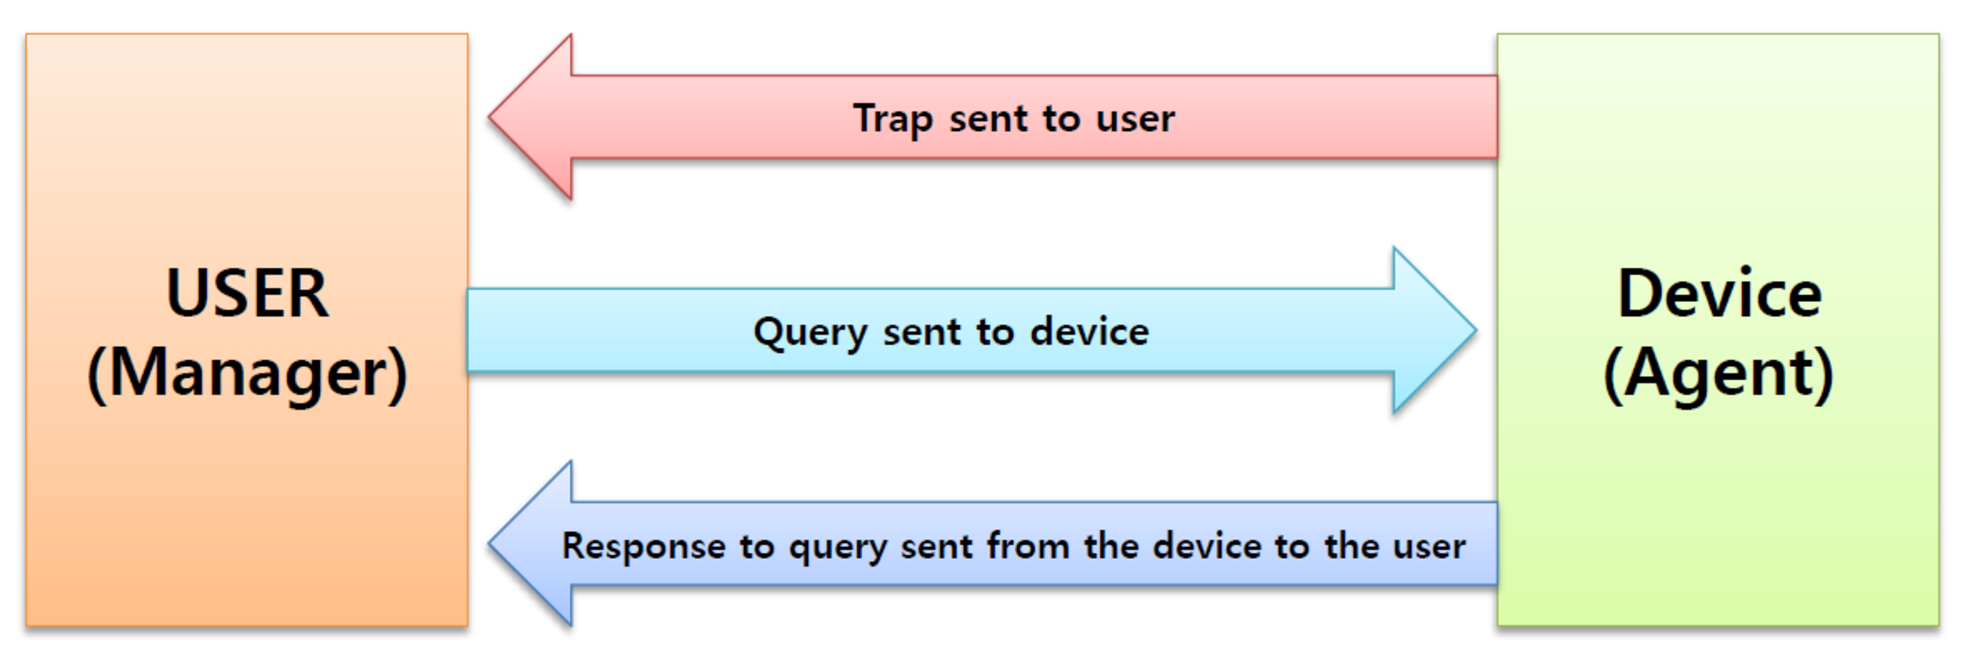
\includegraphics[width=0.65\textwidth]{./images/relationship_m_a.eps}
  \caption{Manager와 Agent의 관계}
  \label{fig:relationship_m_a}   
\end{figure}

\section{EPICS와 SNMP의 융합 필요성 및 계획}
가속기 제어 시스템에 사용되는 대부분 장비가 Ethernet 네트워크를 통하여 연결되며, 모든 네트워크 장비들은 또한 SNMP를 지원하므로 SNMP와 EPICS의 융합은 중이온가속기 중앙 제어 시스템의 일관성, 유지관리의 용이성, 그리고 최적화 기술의 습득 및 축적의 관점에서 중요하다. 또한, 이는 하나의 서버로 많은 수의 SNMP지원 장비를 모니터링할 수 있으며, 서버의 증설이 쉽고, 문제 발생 시 교체도 쉽다. 따라서 이미 타가속기 사이트에 맞춰 개발된 devSNMP가 아닌 중이온가속기에 최적화된 융합 시스템 개발한다. 그림 \ref{fig:architecture}은 EPICS와 SNMP 융합시스템의 구조이다. 본 장에서 개발할 융합 시스템에서 모니터링 및 제어될 장비는 SNMP MIB를 통해 EPICS와 연결되고, 이는 IOC로 개발되어 CA를 통해 PV와 장비를 통신할 수 있게 한다. PV는 MIB가 가진 장비의 정보로 장비의 모니터링 및 제어에 사용된다\citep{epicssnmp}. 

\begin{figure}[h!]
  \centering
  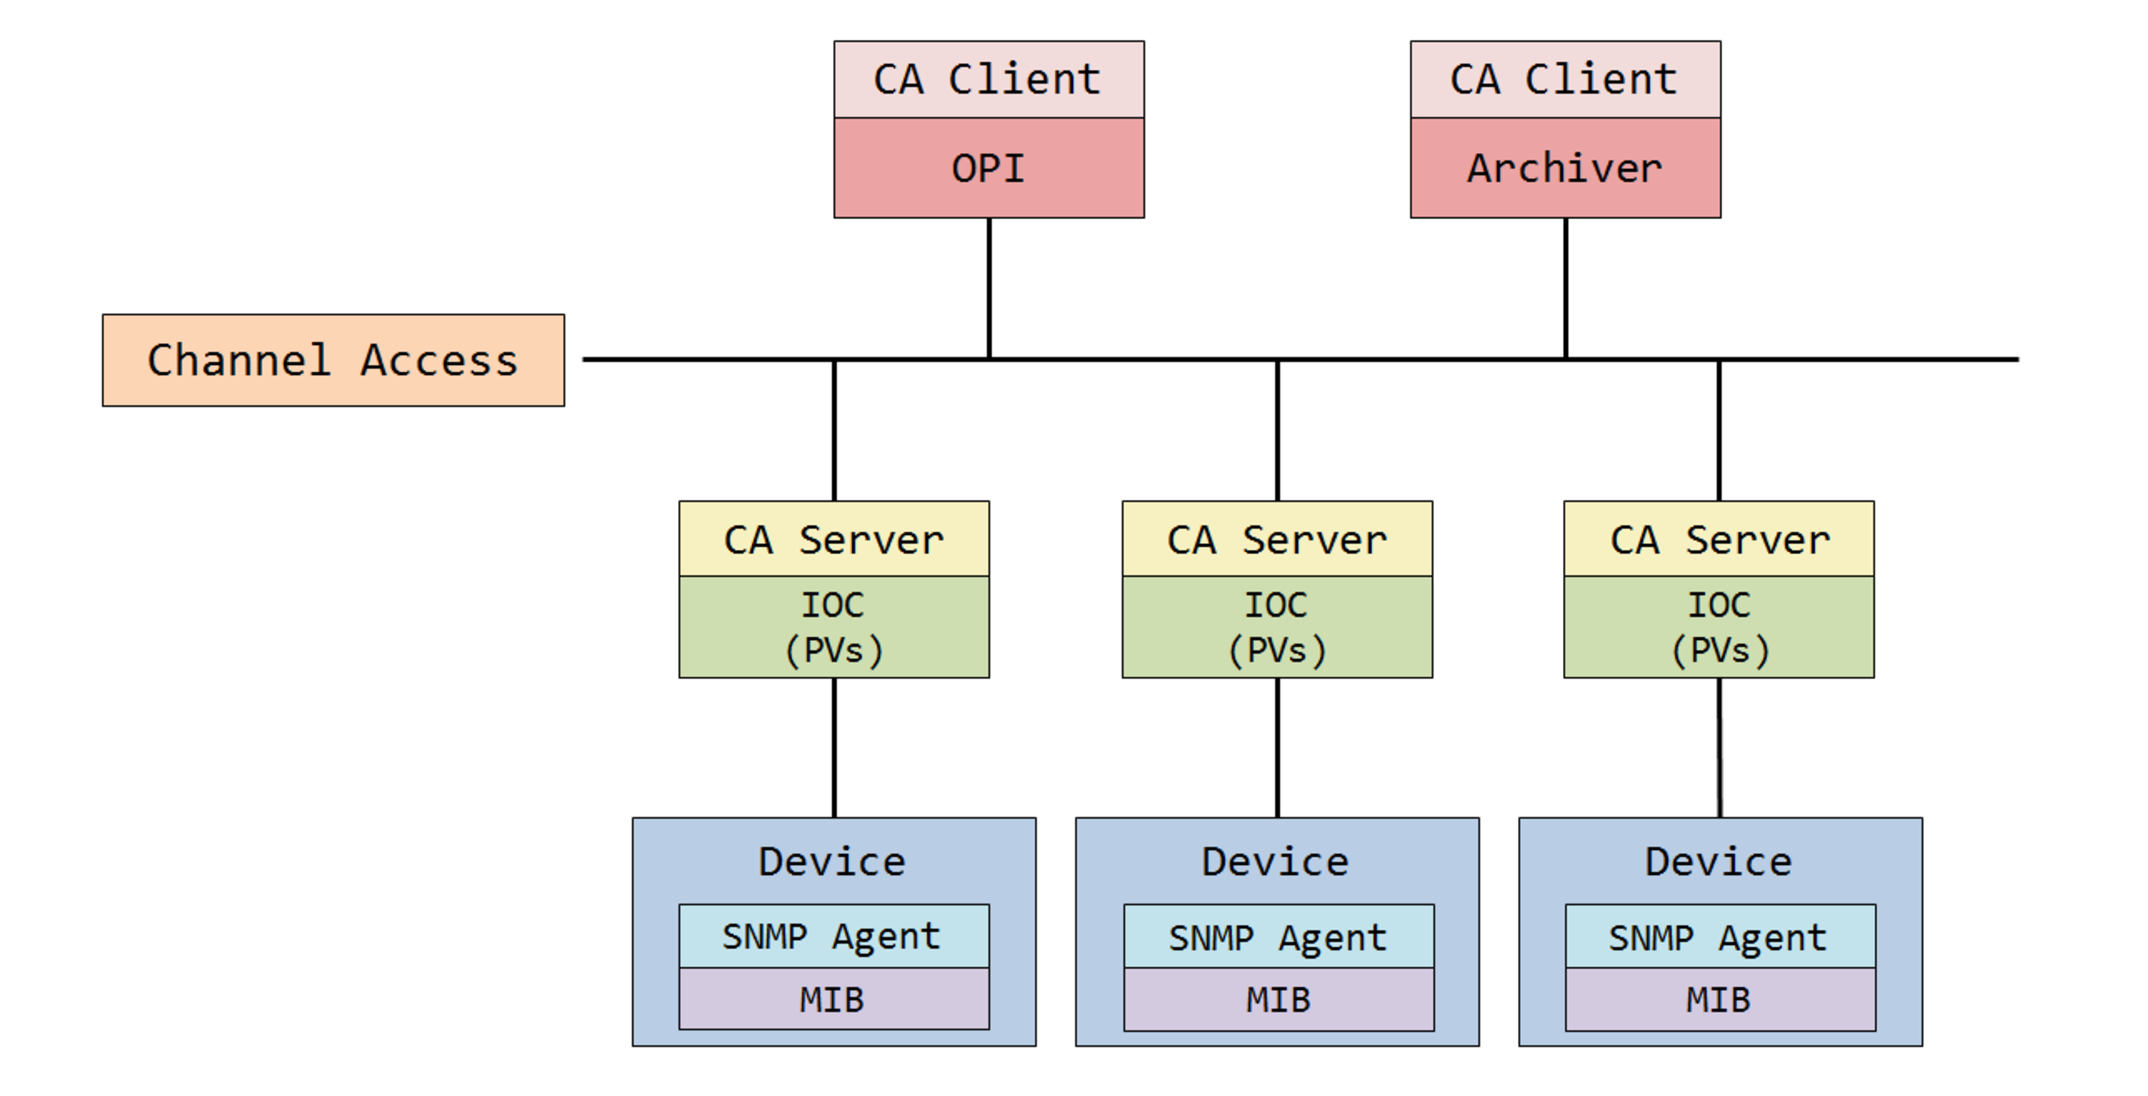
\includegraphics[width=0.79\textwidth]{./images/architecture.eps}
  \caption{EPICS와 SNMP 통합 시스템 아키텍처}
  \label{fig:architecture}   
\end{figure}

\chapter{EPICS IOC Support Modules}
EPICS IOC Support Module은 다른 인터페이스를 가진 하드웨어에 따라 새로운 타입의 레코드나 소프트웨어를 지원하는 Module인 Soft Support와 IOC 내에서 사용 가능한 하드웨어를 지원하는 Module인 Hardware Support로 분류된다. SNMP Soft Support Module은 이미 EPICS Community 내 다수의 개발자에 의해 개발된 devSNMP와 이를 보완한 snmp-nscl이 존재한다. 본 문서는 NSCL/FRIB의 SNMP Device Support Module(snmp-nscl)을 사용한다\citep{modules}.

\section{NSCL/FRIB SNMP Device Support Module}
NSCL/FRIB SNMP Device Support Module (이하 snmp-nscl)은 EPICS에서 SNMP를 통한 하드웨어 장비와의 통신을 위해 2004년 LANL\footnote{* Los Alamos National Laboratory}의 Richard Dubney에 의해 최초 개발된 후 DESY\footnote{* Deutsches Elektronen-Synchrotron}의 Albert Kagarmanov에 의해 개발된 devSNMP를 기반으로 NSCL\footnote{* National Superconducting Cyclotron Laboratory}/FRIB\footnote{* Facility for Rare Isotope Beams}의 John Priller에 의해 개발되었다. DESY의 devSNMP는 snmpv1/2c와 Read만을 지원했다. 이에 devSNMP 코드를 기반으로 snmpv1/2c/3과 Read/ Write를 지원하는 snmp-nscl이 개발되었고, 이는 현재 Wiener/ISEG/MPOD power supply crates에 초점을 두고 RC9 버전까지 개발되었으며, SNMPv2에 최적화 되어있다\citep{devsnmp}. 

\subsection{사용 방법}
snmp-nscl을 사용하여 SNMP를 통해 하드웨어와 EPICS가 통신하기 위해서는 Net-SNMP library와 SNMP를 지원하는 장비, 그리고 장비의 MIB파일이 필요하다. MIB는 보통 리눅스 시스템에서 아래의 경로에 있다.

\begin{lstlisting}[style=termstyle]
/usr/local/share/snmp/mibs/ 
/usr/share/mibs
\end{lstlisting}

devSNMP는 OID의 데이터 타입과 Access 권한에 따라 아래의 레코드 타입을 지원한다.

\begin{itemize}
\item Input\\
 - ai (Analog Input)\\
 - longin (Long Input)\\
 - string in (String Input)\\
 - waveform (DBF\_STRING, DBF\_CHAR, DBF\_UCHAR)
 
\item Output\\
 - ai (Analog Output)\\
 - longout (Long Output)\\
 - ­stringout (Stirng Output)
\end{itemize}

레코드는 디바이스 타입, 스캔 시간, 초기화 등의 다양한 필드를 가진다\footnote{* 각 레코드 및 필드에 대한 정의는 EPICS Record Reference Manual\citep{record}을 참조 바란다}. devSNMP를 사용하는 레코드의 포맷은 다음과 같다. 레코드의 필드 중 INP/OUT의 포맷은 SNMP 명령어와 유사하다는 것을 알 수 있다. 이는 Read의 경우 INP필드에 장비의 Host, Community string, 객체의 이름 등의 정보를 정의하고, Write의 경우 OUT필드에 데이터 타입에 따른 set\_type을 추가 정의해야 한다.

\begin{lstlisting}[style=termstyle]
record(record type, "PV Name") {
 field(DESC, "Description")
 field(DTYP, "Device Type")
 field(SCAN, "Scan rate")
 field(PREC, "Display Precision")
 field(INP/OUT, "@host community OIDname mask dataLength [set_type[special_flags]]")
 .
 .
 }
\end{lstlisting}

아래는 APC사의 PDU의 Voltage에 대해 ai/ao 타입으로 정의한 레코드의 예로 이는 VoltageRead, VoltageSet의 PV 이름을 가지고 CA를 통해 EPICS IOC와 통신하여 장비의 Voltage 값을 모니터링 및 변경할 수 있다.

\begin{lstlisting}[style=termstyle]
   record(ai, "VoltageRead") {
     field(DESC, "SNMP channel")
     field(DTYP, "Snmp")
     field(SCAN, ".2 second")
     field(PREC, "3")
     field(INP, "@host community WIENER-CRATE-MIB::outputMeasurementSenseVoltage.u0 Float: 100")
   }

   record(ao, "VoltageSet") {
     field(DESC, "SNMP channel")
     field(DTYP, "Snmp")
     field(SCAN, "Passive")
     field(PREC, "3")
     field(OUT, "@host community WIENER-CRATE-MIB::outputVoltage.u0 Float: 100 F")
   }
\end{lstlisting}

각 record는 객체의 Access 권한과 데이터 타입에 따라 VoltageRead, VoltageSet의 이름으로 DB 파일에 정의되고, 이는 PV가 되어 CA를 통한 EPICS와 하드웨어의 통신이 가능해지므로, Voltage 값 변경 및 모니터링을 할 수 있다.

\section{devSNMP를 이용한 프린터 모니터링 시스템 개발}
본 문서에서는 중이온가속기 제어 환경에 최적화된 EPCIS와 SNMP 융합 제어 시스템 개발에 앞서 EPICS 사용 및 IOC, DB 설계 및 CSS를 사용한 UI 구성 등의 경험 축적을 위해 devSNMP vRC8을 사용한 통합 모니터링 시스템 초기 버전을 개발한다. 이는 가속기 제어에 사용되는 다양한 장비 적용에 앞서 사무실 내의 네트워크 프린터기에 적용한다. 프린터 모니터링 시스템 구축에 사용된 소프트웨어와 하드웨어는 다음과 같다.

\begin{itemize}
\item Debian Linux 7 Wheezy
\item NET-SNMP v5.4.3
\item EPICS v3.14.12.4
\item NSCL/FRIB devSNMP vRC8
\item CSS (Control System Studio) v3.2.13a
\item Printers(XEROX ApeosPort-IV C3375, KYOCERA FS-9530DN)
\end{itemize}

\subsection{Customized Device Support Module}
중이온가속기 EPICS 개발 환경은 1장 2절과 같이 소프트웨어의 효율적인 재사용을 위한 siteLibs와 IOC를 개발하는 siteApps로 분리된 구조를 가진다. devSNMP는 <표 4-3>과 같이 Db와 src가 통합된 기본 구조를 가지고 있다. 따라서 이를 중이온가속기 제어 개발 환경과 프린터 모니터링 환경에 맞추기 위해 siteLibs와 siteApps에 맞는 구조로 변경이 필요하다.

{\scriptsize
\begin{verbatim}
.
├── configure
├── documentation
├── iocBoot
├── Makefile
├── mibs
├── snmpApp
│   ├── Db
│   ├── Makefile
│   └── src
└── WienerCrate
\end{verbatim}
}

\subsubsection{$ \circ $ Library(siteLibs) 구조화}
앞서 언급했듯 기존의 devSNMP는 목적과 객체의 접근권한에 따라 다양한 레코드 타입을 제공하지만, 중이온가속기의 Library 환경과 프린터 모니터링 환경에 맞추기 위해 독자적인 레코드 생성 및 소스코드의 수정이 필요하다.\\

①  레코드\\
- snmpMSURecord.dbd/snmpMSURecord.c\\
EPICS의 Example IOC Application의 기본 레코드 필드를 활용하여 SNMP 데이터 타입 중 string을 지원할 snmpstr 레코드와 그 외의 데이터 타입에서 사용될 snmp 레코드를 생성한다. 그리고 snmp 레코드에는 종이, 잉크의 잔량을 퍼센트(\%)로 표현하기 위해 사칙연산 메뉴와 이를 사용할 MJP 필드, 그리고 Double 타입의 SVAL, OVAL 필드를 추가한다.

{\scriptsize
\begin{lstlisting}[style=termstyle]
#ifndef INCmenuCalcH
#define INCmenuCalcH
typedef enum {
	menu_Plus,
	menu_Minus,
	menu_Mul,
	menu_Div
}menuCalc;
#endif /*INCmenuCalcH*/
#ifndef INCsnmpH
#define INCsnmpH
typedef struct snmpRecord {
	epicsFloat64	val;	/* Desired Output */
	epicsFloat64	sval;	/* Extra Value */
	epicsFloat64	oval;	/* Percentage Value */
          epicsEnum16         mjp;      /* Operation menu */

	DBLINK		inp;	/* Input Specification */
	DBLINK		out;	/* Output Specification */
{...}
} snmpRecord;

#ifndef INCsnmpstrH
#define INCsnmpstrH
typedef struct snmpstrRecord {
	char		val[40];	/* Current Value */
	DBLINK		out;	/* Output Specification */
{...}
} snmpstrRecord;
\end{lstlisting}
}

\hfill

②  소스코드\\
앞서 생성한 레코드를 사용하기 위해 세 가지 파일을 수정한다.\\

- devSnmpSoft.cpp\\
생성한 레코드의 dset(Address of Device Support Entry Table)을 선언하고, 기존의 정보를 읽어오는 함수에 사칙연산을 위한 코드를 추가한다. 아래의 코드는 devSnmpSoft.cpp의 일부이다.

{\scriptsize
\begin{lstlisting}[style=termstyle]
static struct {
  long            number;
{...}
  DEVSUPFUN       write_snmp;
  DEVSUPFUN       special_linconv;
} devSnmpSoft = {
  6,
{...}
  (DEVSUPFUN) snmpSoftWrite,
  NULL
};
epicsExportAddress(dset,devSnmpSoft);
static struct {
  long       number;
{...}
  DEVSUPFUN  write_snmpstr;
  DEVSUPFUN  special_linconv;
} devSnmpstrSoft = {
  6,
  NULL,
{...}
  (DEVSUPFUN) snmpstrSoftWrite,
  NULL
};
epicsExportAddress(dset,devSnmpstrSoft);
\end{lstlisting}
}

{\scriptsize
\begin{lstlisting}[style=termstyle]
static long snmpSoftReadback(devSnmp_pv *pPV)
{
  struct snmpRecord *psnmp = (struct snmpRecord *) pPV->record();
  epicsStatus status = epicsError;
  double new_val;
{...}
        psnmp->rval = new_val;
        char oval[40]; 
        char sval[40]; //percent
        switch(psnmp->mjp)
        {
                case menu_Plus: 
                psnmp->val = ceil(psnmp->rval+psnmp->oval*psnmp->sval);
                break;
                case menu_Minus: 
                psnmp->val = ceil(psnmp->rval-psnmp->oval*psnmp->sval);
                break;
                case menu_Mul: 
                psnmp->val = ceil(psnmp->rval*psnmp->oval*psnmp->sval);
                break;
                case menu_Div: 
                psnmp->val = ceil(psnmp->rval/psnmp->oval*psnmp->sval);
                break;
        }
        process_record = true;
      }
    }
{...}
  // process record if needed
  if (process_record) pPV->processRecord();

  return(status);
}
\end{lstlisting}
}

\hfill

- snmpMSUDevSoft.dbd\\
선언한 dset을 dbd파일에 추가한다.\\
{\scriptsize
\begin{lstlisting}[style=termstyle]
static long snmpSoftReadback(devSnmp_pv *pPV)
{
  struct snmpRecord *psnmp = (struct snmpRecord *) pPV->record();
  epicsStatus status = epicsError;
  double new_val;
{...}
        psnmp->rval = new_val;
        char oval[40]; 
        char sval[40]; //percent
        switch(psnmp->mjp)
        {
                case menu_Plus: 
                psnmp->val = ceil(psnmp->rval+psnmp->oval*psnmp->sval);
                break;
                case menu_Minus: 
                psnmp->val = ceil(psnmp->rval-psnmp->oval*psnmp->sval);
                break;
                case menu_Mul: 
                psnmp->val = ceil(psnmp->rval*psnmp->oval*psnmp->sval);
                break;
                case menu_Div: 
                psnmp->val = ceil(psnmp->rval/psnmp->oval*psnmp->sval);
                break;
        }
        process_record = true;
      }
    }
{...}
  // process record if needed
  if (process_record) pPV->processRecord();

  return(status);
}
\end{lstlisting}
}

\hfill

③ Makefile\\
Library로 만들 소스코드 정의와 Net-SNMP 사용을 위한 설정을 추가한다.\\
{\scriptsize
\begin{lstlisting}[style=termstylenumber]
TOP = ../..
include $(TOP)/configure/CONFIG

LIBRARY      += devSnmp  
DBD          += snmpMSURecord.dbd
DBDINC       += snmpMSURecord
DBD          += menuCalc.dbd
DBDINC       += menuCalc
devSnmp\_SRCS += snmpRegister.cpp snmpSessShow.c devSnmpSoft.cpp snmpMSURecord.c

USR\_CFLAGS   += `net-snmp-config -cflags`
USR\_LDFLAGS  += `net-snmp-config --libs`
PROD\_LDLIBS  += `net-snmp-config --libs`

USR\_CFLAGS   += $(shell $(PERL) ../getNetSNMPversion.pl)
USR\_CPPFLAGS += $(shell $(PERL) ../getNetSNMPversion.pl)

DBD          += snmpMSUDevSoft.dbd

include $(TOP)/configure/RULES
\end{lstlisting}
}

\hfill

\subsubsection{$ \circ $ Application(siteApps) 구조화}

Library를 사용해 IOC를 실행하기 위한 application은 디렉토리를 생성 후 아래와 같이 makeBaseApp.pl을 사용해 Application IOC boot를 만든다.

{\scriptsize
\begin{lstlisting}[style=termstyle]
mijoy0909@mjpark:~/epics/R3.14.12.4/siteApps/snmpMSU/$ makeBaseApp.pl -t ioc snmp 
mijoy0909@mjpark:~/epics/R3.14.12.4/siteApps/snmpMSU/$ makeBaseApp.pl -i -t ioc snmp
The following applications are available:
    snmp
What application should the IOC(s) boot?
The default uses the IOC's name, even if not listed above.
Application name? snmp
mijoy0909@mjpark:~/epics/R3.14.12.4/siteApps/snmpMSU/$ make
\end{lstlisting}
}

\hfill

위의 과정을 거치면 devSNMP는 Library화 되어 아래와 같은 구조가 된다. 
{\scriptsize
\begin{verbatim}
.
├── Makefile
└── src
    ├── devSnmp.h
    ├── devSnmpSoft.cpp
    ├── getNetSNMPversion.pl
    ├── Makefile
    ├── menuCalc.dbd
    ├── requireNetSNMPversion.h
    ├── snmp.h
    ├── snmpMSUDevSoft.dbd
    ├── snmpMSURecord.c
    ├── snmpMSURecord.dbd
    ├── snmpRegister.cpp
    └── snmpSessShow.c
\end{verbatim}
}

\hfill

-­ Makefile\\
snmpApp/src의 Makefile에 앞서 만든 Library의 경로와 사용할 파일을 추가한다. 

{\scriptsize
\begin{lstlisting}[style=termstylenumber]
TOP=../..

include $(TOP)/configure/CONFIG

USR_INCLUDES += -I${RAON_SITELIBS}/include
USR_DBDFLAGS += -I${RAONS_ITELIBS}/dbd          /* add library path */

devSnmp_DIR  += ${RAON_SITELIBS}/lib/$(T_A)

#----------------------------------------
#  ADD MACRO DEFINITIONS AFTER THIS LINE
#=============================
#=============================
# Build the IOC application

PROD_IOC = snmp
# snmp.dbd will be created and installed
DBD += snmp.dbd

# snmp.dbd will be made up from these files:
snmp_DBD  += base.dbd
snmp_DBD  += snmpMSURecord.dbd                    /* add record */

# Include dbd files from all support applications:
#snmp_DBD += xxx.dbd
snmp_DBD  += snmpMSUDevSoft.dbd                   /* add dbd file */

# Add all the support libraries needed by this IOC
#snmp_LIBS += xxx
snmp_LIBS  += devSnmp                             /* add library */

# snmp_registerRecordDeviceDriver.cpp derives from snmp.dbd
snmp_SRCS  += snmp_registerRecordDeviceDriver.cpp

# Build the main IOC entry point on workstation OSs.
snmp_SRCS_DEFAULT += snmpMain.cpp
snmp_SRCS_vxWorks += -nil-

# Add support from base/src/vxWorks if needed
#snmp_OBJS_vxWorks += $(EPICS_BASE_BIN)/vxComLibrary

# Finally link to the EPICS Base libraries
snmp_LIBS  += $(EPICS_BASE_IOC_LIBS)

#===========================

include $(TOP)/configure/RULES
#----------------------------------------
#  ADD RULES AFTER THIS LINE
\end{lstlisting}
}

\hfill

-­ Db\\
snmpApp/Db 디렉토리에 레코드 정보를 담은 Db파일을 생성한다. 이는 VisualDCT (VDCT) 또는 에디터프로그램으로 작성할 수 있다. VDCT의 경우 Db파일은 .vdb의 확장자를 가진다. 아래는 Xerox사 프린터 Db파일의 일부로 토너(Black, Yellow)에 대한 레코드이다. devSNMP의 필드 포맷에 맞춰 OUT 필드를 작성하였다. 그리고 VAL 값인 토너의 잔량을 퍼센트로 표현하기 위해 MJP, OVAL, SVAL 필드를 사용하였다. 

{\scriptsize
\begin{lstlisting}[style=termstyle]
record(snmp, "${USER}:xerox_toner_B") {
  field(DESC, "xeorx toner")
  field(SCAN, "Passive")
  field(DTYP, "SoftChannel")
  field(OUT, "@%(XEROX) %(CM2) %(PR)prtMarkerSuppliesLevel.1.1  INTEGER: 100 ")
  field(MJP, "Division")
  field(OVAL, "26000")              /* the overall amount of black toner */ 
  field(SVAL, "100")
}

record(snmp, "${USER}:xerox_toner_Y") {
  field(DESC, "xeorx toner")
  field(SCAN, "Passive")
  field(DTYP, "SoftChannel")
  field(OUT, "@%(XEROX) %(CM2) %(PR)prtMarkerSuppliesLevel.1.2  INTEGER: 100 ")
  field(MJP, "Division")
  field(OVAL, "15000")             /* the overall amount of yellow toner */
  field(SVAL, "100")
}
\end{lstlisting}
}


\hfill

생성한 Db파일을 Makefile에 추가한다.

{\scriptsize
\begin{lstlisting}[style=termstylenumber]
TOP=../..
include $(TOP)/configure/CONFIG
#----------------------------------------
#  ADD MACRO DEFINITIONS AFTER THIS LINE

#----------------------------------------------------
#  Optimization of db files using dbst (DEFAULT: NO)
#DB_OPT = YES

#----------------------------------------------------
# Create and install (or just install) into <top>/db
# databases, templates, substitutions like this
#DB += xxx.db
DB += printer.vdb                 /*  add Db file */

#----------------------------------------------------
# If <anyname>.db template is not named <anyname>*.template add
# <anyname>_template = <templatename>

include $(TOP)/configure/RULES
#----------------------------------------
#  ADD RULES AFTER THIS LINE
\end{lstlisting}
}


\hfill

 Application을 make한다.

{\scriptsize
\begin{lstlisting}[style=termstyle]
mijoy0909@mjpark:~/epics/R3.14.12.4/siteApps/snmpMSU$ make
\end{lstlisting}
}



\hfill

make 후 디렉토리에 bin, db, dbd 디렉토리가 생성되고, 각 폴더에는 siteLibs과 마찬가지로 IOC 실행에 사용될 파일이 생성된다. 위의 과정을 거친 Application은 다음과 같은 구조를 가진다. 프린터의 MIB  파일은 mibs 디렉토리에 넣어둔다.

{\scriptsize
\begin{verbatim}
.
├── bin
├── configure
├── db
├── dbd
├── iocBoot
├── Makefile
├── mibs
└── snmpApp
\end{verbatim}
}




\hfill

-­ st.cmd\\
/iocBoot/iocsnmp로 이동 후 앞서 생성한 Db파일을 st.cmd파일에 추가해준다. 이때, MIB파일의 경로, 사용하고자 하는 SNMP의 버전, 매크로 값에 대한 정보를 추가한다. 





{\scriptsize
\begin{lstlisting}[style=termstyle]
#!../../bin/linux-x86_64/snmp

## You may have to change snmp to something else
## everywhere it appears in this file

< envPaths

cd ${TOP}

epicsEnvSet("MIBDIRS", "+$(TOP)/mibs")                     
devSnmpSetSnmpVersion("10.1.4.184","SNMP_VERSION_1")        
devSnmpSetSnmpVersion("10.1.4.182","SNMP_VERSION_2c")       

epicsEnvSet("PR", "Printer-MIB::")                           
epicsEnvSet("JM", "Job-Monitoring-MIB::")                     
epicsEnvSet("SMI", "SNMPv2-SMI::")
epicsEnvSet("XM", "XEROX-SERVICE-MONITORING-MIB::")        
epicsEnvSet("CM1", "admin")                               
epicsEnvSet("CM2", "public")
epicsEnvSet("XEROX", "10.1.4.182")
epicsEnvSet("KYOCERA", "10.1.4.184")                                           

## Register all support components
dbLoadDatabase "dbd/snmp.dbd"
snmp_registerRecordDeviceDriver pdbbase

## Load record instances
dbLoadRecords("db/printer.vdb","USER=mijoy0909Host")        

cd ${TOP}/iocBoot/${IOC}
iocInit

## Start any sequence programs
#seq sncxxx,"user=mijoy0909Host"
\end{lstlisting}
}


\hfill

st.cmd파일에 실행권한을 부여 후 실행한다. 
{\scriptsize
\begin{lstlisting}[style=termstyle]
mijoy0909@mjpark:~/epics/R3.14.12.4/siteApps/snmpMSU/iocBoot/iocsnmp$ chmod 755 st.cmd
\end{lstlisting}
}

\hfill

IOC 실행 후 생성한 PV 리스트를 확인한 결과는 다음과 같다. 

{\scriptsize
\begin{lstlisting}[style=termstyle]
cd /home/mijoy0909/epics/R3.14.12.5/siteApps/snmpMSU/iocBoot/iocsnmp
iocInit
Starting iocInit
############################################################################
## EPICS R3.14.12.5 $Date: Tue 2015-03-24 09:57:35 -0500$
## EPICS Base built Apr  6 2015
############################################################################
iocRun: All initialization complete
## Start any sequence programs
#seq sncxxx,"user=mijoy0909Host"
epics> dbl
mijoy0909Host:kyocera_TR1
mijoy0909Host:kyocera_TR2
mijoy0909Host:kyocera_TR3
mijoy0909Host:kyocera_TR4
mijoy0909Host:kyocera_TR5
mijoy0909Host:kyocera_active
mijoy0909Host:kyocera_length1
mijoy0909Host:kyocera_length2
mijoy0909Host:kyocera_length3
mijoy0909Host:kyocera_length4
mijoy0909Host:kyocera_length5
mijoy0909Host:kyocera_power
mijoy0909Host:kyocera_toner
mijoy0909Host:kyocera_width1
mijoy0909Host:kyocera_width2
mijoy0909Host:kyocera_width3
mijoy0909Host:kyocera_width4
mijoy0909Host:kyocera_width5
mijoy0909Host:xerox_TR1
mijoy0909Host:xerox_TR2
mijoy0909Host:xerox_TR3
mijoy0909Host:xerox_TR4
mijoy0909Host:xerox_TR5
mijoy0909Host:xerox_length1
mijoy0909Host:xerox_length2
mijoy0909Host:xerox_length3
mijoy0909Host:xerox_length4
mijoy0909Host:xerox_length5
mijoy0909Host:xerox_power
mijoy0909Host:xerox_toner_B
mijoy0909Host:xerox_toner_C
mijoy0909Host:xerox_toner_M
mijoy0909Host:xerox_toner_Y
mijoy0909Host:xerox_toner_drum_B
mijoy0909Host:xerox_toner_drum_C
mijoy0909Host:xerox_toner_drum_M
mijoy0909Host:xerox_toner_drum_Y
mijoy0909Host:xerox_waste
mijoy0909Host:xerox_width1
mijoy0909Host:xerox_width2
mijoy0909Host:xerox_width3
mijoy0909Host:xerox_width4
mijoy0909Host:xerox_width5
mijoy0909Host:kyocera_state
mijoy0909Host:xerox_print
mijoy0909Host:xerox_state
mijoy0909Host:xerox_state_sub
epics> 
\end{lstlisting}
}

\hfill

PV가 장비와 통신 되고 있는지 확인하기 위해 EPICS의 Command, CA monitor, snmpget을 값을 확인한 결과 모두 같은 값을 보이므로  SNMP를 통해 EPICS IOC와 프린터가 통신함을 확인할 수 있다.  

\begin{itemize}
\item EPICS IOC Command\\
{\scriptsize
\begin{lstlisting}[style=termstyle]
epics> dbpr mijoy0909Host:xerox_state
ASG:      DESC: SNMP channel  DISA: 0          DISP: 0             
DISV: 1    NAME: mijoy0909Host:xerox_state        SEVR: NO_ALARM      
STAT: NO_ALARM      TPRO: 0                   VAL: Printing...    
\end{lstlisting}
}
\item CA Monitor\\
{\scriptsize
\begin{lstlisting}[style=termstyle]
mijoy0909@mjpark:~$ camonitor mijoy0909Host:xerox_state
mijoy0909Host:xerox_state      2015-03-19 15:23:32.007583 Printing...  
\end{lstlisting}
}
\item snmpget\\
{\scriptsize
\begin{lstlisting}[style=termstyle]
mijoy0909@mjpark:~$ snmpget -v 2c -c public 10.1.4.182 prtConsoleDisplayBufferText.1.1
Printer-MIB::prtConsoleDisplayBufferText.1.1 = STRING: "Printing..."
\end{lstlisting}
}
\end{itemize}

\clearpage

\subsection{프린터 모니터링 시스템 UI 개발}
수정된 Lib/App을 통해 EPICS IOC를 통한 모니터링 시스템을 구축하였고, End-User에게 더 나은 환경을 제공하기 위해 사무실 환경 모니터링과 함께 프린터의 상태, 소모품의 잔량 등의 정보 확인 및 종이 걸림, 소모품 부족 등의 알림을 확인할 수 있도록 CSS를 사용한 OPI를 개발하였다. CSS의 스크린 캡처와 실제 구동화면은 그림 \ref{fig:css_op}와 그림 \ref{fig:css_monitoring}에서 살펴볼 수 있다.

\begin{figure}[h!]
  \centering
  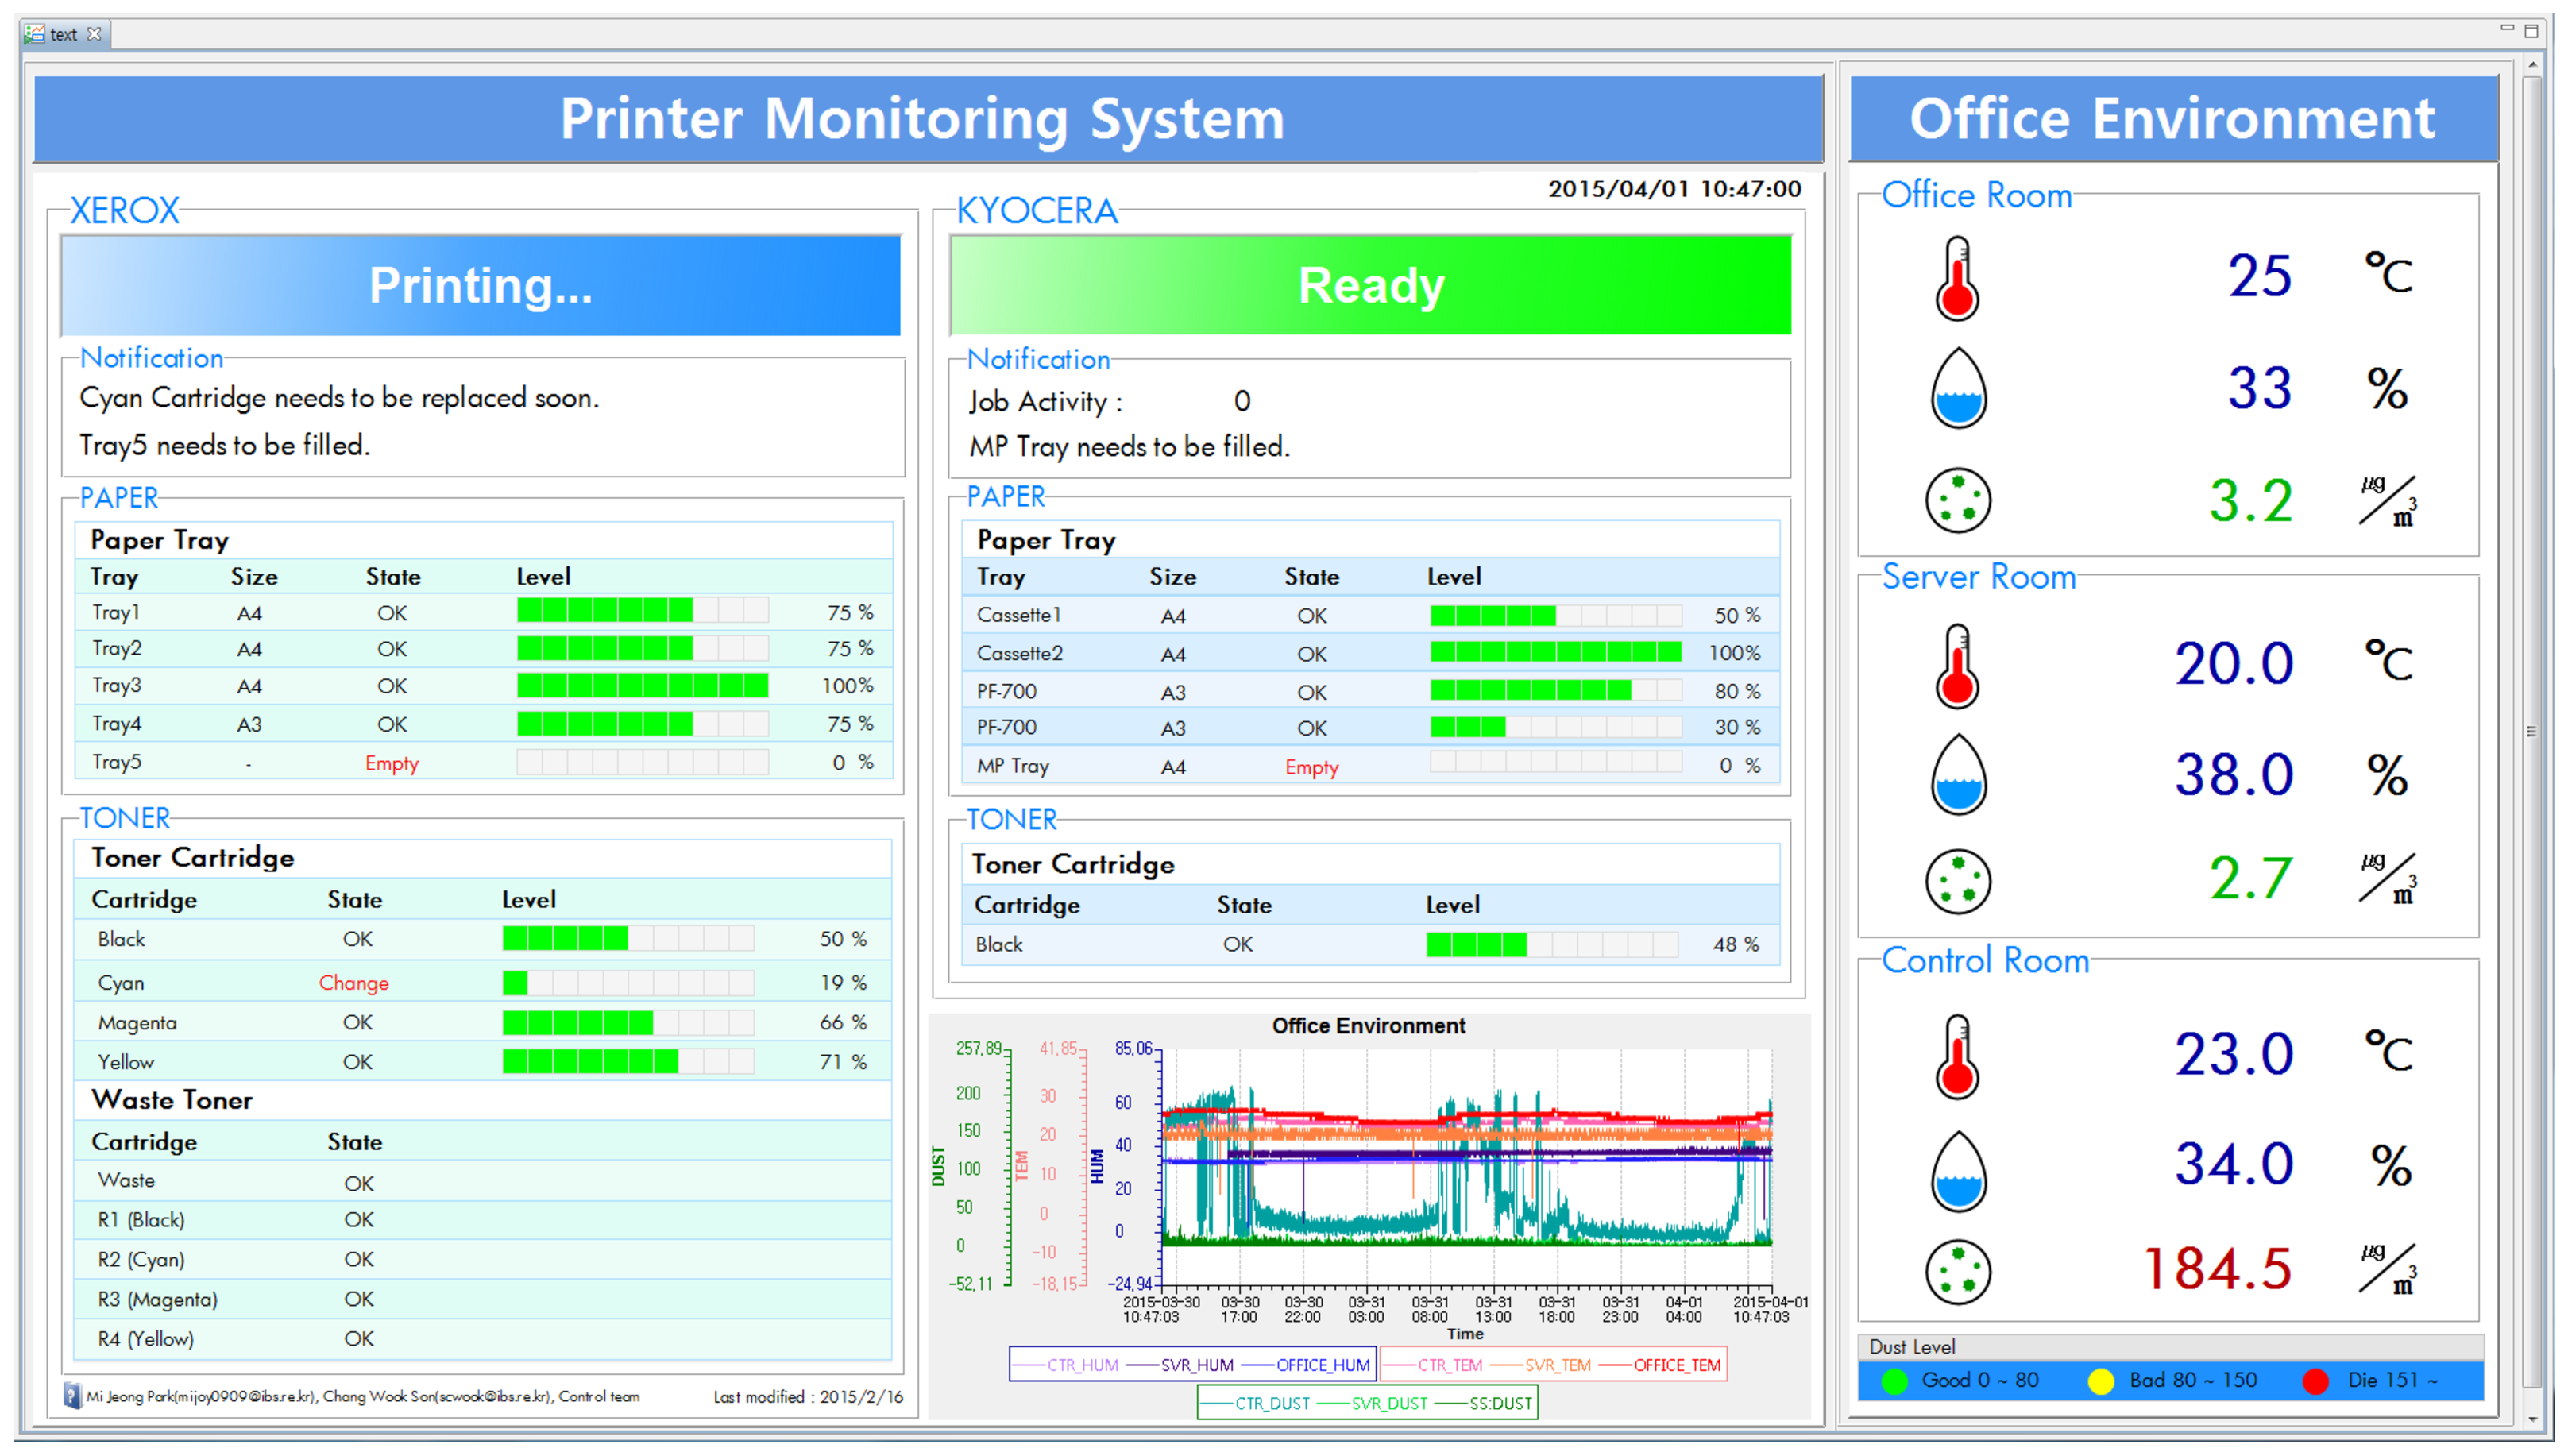
\includegraphics[width=0.7\textwidth]{./images/css_op.eps}
  \caption{프린터 모니터링 시스템 실제 구동화면}
  \label{fig:css_op}   
\end{figure}


\begin{figure}[h!]
  \centering
  \includegraphics[width=0.7\textwidth]{./images/css_monitoring.eps}
  \caption{프린터 모니터링 시스템 실제 구동화면}
  \label{fig:css_monitoring}   
\end{figure}

\subsection{devSNMP의 장·단점 및 문제점}
devSNMP는 EPICS Community 내에서 오랜 개발로 안정성이 검증 및 현재 개발 중이다. 이는 모듈 파라미터 구성과 문제를 진단하는 데 도움이 되는 IOC Shell Commands를 제공한다. 또한, SNMP의 다양한 데이터 타입(Integer, String, Gauge, IP Address 등)을 모두 지원한다. 하지만 SNMPv2c에 최적화되어 있는 devSNMP는 구체적인 v3에 지원이 필요하다. 또한, 데이터 타입에 따라 mask와 data length 값을 설정해야 하는 불편함이 존재한다. 현재 devSNMP는 몇 가지 버그가 존재한다. 이는 Wiener/ISEG/MPOD사의 장비에서 가끔 반환되는 데이터 값과 실제 값의 차이, 요구되는 데이터가 아닌 다른 변수의 반환 등이다.

\chapter{RAON에 최적화된 EPICS와 SNMP 융합 시스템}
중이온가속기에 최적화된 융합 시스템을 개발하는데 있어  Net-SNMP API 코드들을 사용하였으며, 응답속도와 보안에 효율적인 방법으로 모니터링(Read)에는 SNMPv2c, 제어(Write)에는 SNMPv3에 최적화하여 개발을 진행하였다. 연구에 사용한 소프트웨어와 하드웨어는 다음과 같다. 통합에 사용한 소프트웨어와 하드웨어는 그림 \ref{fig:integ2}과 같다.

\begin{figure}[h!]
  \centering
  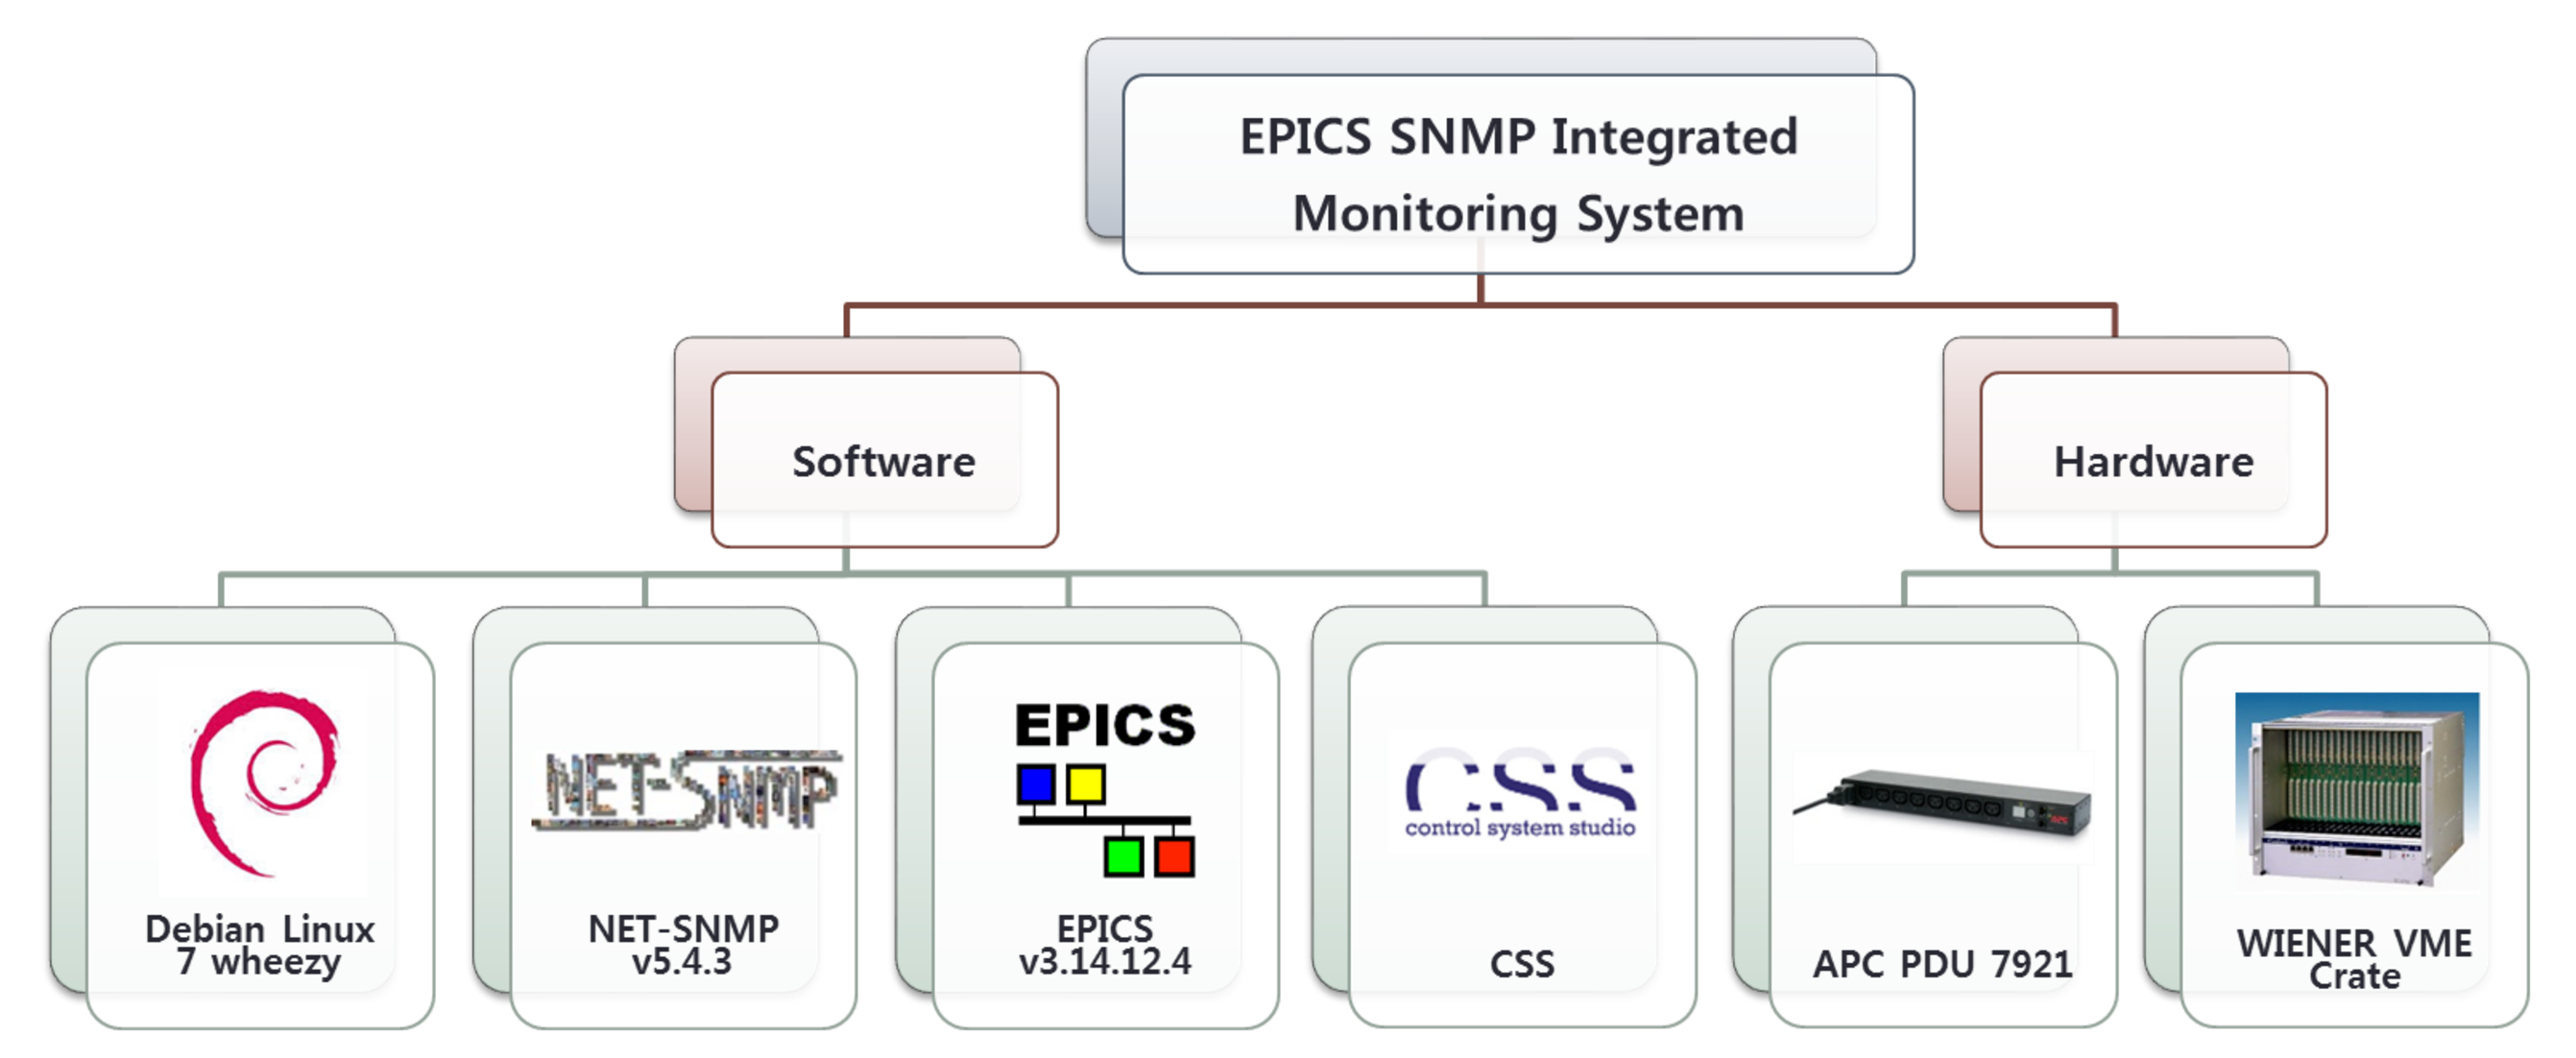
\includegraphics[width=0.99\textwidth]{./images/integ.eps}
  \caption{모니터링 시스템의 구성}
  \label{fig:integ2}   
\end{figure}


\section{Pretest with SNMP API Code}
Net-SNMP에서 제공하는 Tutorial 예제 중 Client/Manager Coding Tutorials는 동기식의 Simple application(이하 Sync)과 비동기식의 Simple Async Application(이하 Async)으로 구성되어있다. 이에 본 절에서는 EPICS와의 융합에 적합한 SNMP의 응답 방식을 찾기 위해 API Code를 사용한 Sync 및 Async에 대한 간단한 테스트를 진행한다. 

\clearpage

\begin{itemize}
\item (a)Sync 결과\\
{\scriptsize
\begin{lstlisting}[style=termstyle]
---------- synchronous -----------
14:48:31.666708 Kyocera: RFC1213-MIB::sysObjectID.0 = OID: KYOCERA-MIB::kyocera.41
14:48:31.667085 Kyocera: RFC1213-MIB::ifAdminStatus.1 = INTEGER: up(1)
14:48:31.693733 Xerox: RFC1213-MIB::sysObjectID.0 = OID: SNMPv2-SMI::enterprises.297.1.11.93.1.35.20.5.3
14:48:31.696660 Xerox: RFC1213-MIB::ifAdminStatus.1 = INTEGER: up(1)
14:48:31.720208 localhost: RFC1213-MIB::sysObjectID.0 = OID: SNMPv2-SMI::enterprises.8072.3.2.10
14:48:31.720429 localhost: RFC1213-MIB::ifAdminStatus.1 = INTEGER: up(1)
\end{lstlisting}
}
\item (b)Async 결과\\
{\scriptsize
\begin{lstlisting}[style=termstyle]
---------- asynchronous -----------
14:48:31.788910 Xerox: RFC1213-MIB::sysObjectID.0 = OID: SNMPv2-SMI::enterprises.297.1.11.93.1.35.20.5.3
14:48:31.789010 Kyocera: RFC1213-MIB::sysObjectID.0 = OID: KYOCERA-MIB::kyocera.41
14:48:31.789113 localhost: RFC1213-MIB::sysObjectID.0 = OID: SNMPv2-SMI::enterprises.8072.3.2.10
14:48:31.789334 localhost: RFC1213-MIB::ifAdminStatus.1 = INTEGER: up(1)
14:48:31.789403 Kyocera: RFC1213-MIB::ifAdminStatus.1 = INTEGER: up(1)
14:48:31.789427 Xerox: RFC1213-MIB::ifAdminStatus.1 = INTEGER: up(1)
\end{lstlisting}
}
\end{itemize}

위의 두 방식을 모두 확인할 수 있는 Async 예제에 Xerox, Kyocera사의 프린터와 localhost를 Agent로 설정하여 인터페이스 상태와 OID정보를 요청한 결과이다.

(a)의 경우 Kyocera, Xerox사, 그리고 localhost의 Agent 순으로 요청에 대한 응답을 호출하는 반면 (b)의 경우 세 개의 Agent 중 응답이 있는 결과의 순서로 호출한다. 이는 Sync방식이 Agent에 요청을 보내고 응답이 올 때까지 블로킹 되어 대기상태를 유지하는 반면 Async방식은 Agent로부터 요청에 대한 응답이 있을 때 callback 형식으로 호출되어 결과를 출력하기 때문이다. 따라서 EPICS와 SNMP의 융합에는 다양한 네트워크 기반의 장비가 사용되므로 비동기식으로 데이터를 전송하는 Async 방법이 적합하다.



\section{EPICS SNMP 융합 제어시스템 연구 및 개발}

\subsection{Library(siteLibs) 구조화}
EPICS와 융합한 제어 시스템 개발을 위해 중이온가속기 Library 환경에 맞춘 레코드 생성 및 Async코드를 수정한다.

\subsubsection{Record}
- snmpRecord.dbd/snmpstrRecord.dbd \\
3장의 devSNMP의 Library화와 마찬가지로 EPICS의 Example IOC Application의 기본 레코드 필드를 활용하여 다양한 SNMP의 데이터 타입 중 string과 BITS 타입을 지원하는 snmpstrRecord와 그 외의 데이터 타입을 지원하는 snmpRecord를 생성한다. 이때 아래와 같이 두 레코드에 SNMP 사용에 필요한 정보를 레코드의 필드로 생성한다. 이는 devSNMP의 INP/OUT 필드에 정보를 넣던 것과 달리 mask, datalength를 사용하지 않고 각 레코드 마다 다른 SNMP 버전을 사용하기 위해서다. 
각 필드에 대한 정보는 부록을 참고하기 바란다.

{\scriptsize
\begin{lstlisting}[style=termstyle]
typedef struct snmpRecord {
	char		host[81];	/* IP Address */
	char		comm[81];	/* Community */
	char		oids[81];	/* OID Name */
	char		auth[81];	/* auth password */
	char		priv[81];	/* priv password */
	char		vers[81];	/* SNMP Version */
	epicsFloat64	val;	/* Current Value */

{...}
} snmpRecord;

typedef struct snmpstrRecord {
	char		host[81];	/* IP Address */
	char		comm[81];	/* Community */
	char		oids[81];	/* OID Name */
	char		auth[81];	/* auth password */
	char		priv[81];	/* priv password */
	char		vers[81];	/* SNMP Version */
	char		val[40];	/* Current Value */
{...}
} snmpstrRecord;
\end{lstlisting}
}

\hfill

- snmpRecord.c/snmpstrRecord.c\\
Record 생성 후 EPICS의 Example IOC Application의 xxxRecord.c를 수정해 snmpRecord.c와 snmpstrRecord.c를 생성한다. 이때 snmpstrRecord는 snmpRecord와 달리 숫자에 대한 알람을 설정 할 필요가 없으므로 process함수의 checkAlarms부분을 주석처리 한다.

{\scriptsize
\begin{lstlisting}[style=termstyle]
static long process(void *precord)
{
	snmpstrRecord	*psnmpstr = (snmpstrRecord *)precord;
	snmpstrdset	*pdset = (snmpstrdset *)(psnmpstr->dset);
	long		status;
	unsigned char       pact=psnmpstr->pact;

        if( (pdset==NULL) || (pdset->read_snmpstr==NULL) ) {
        psnmpstr->pact=TRUE;
        recGblRecordError(S_dev_missingSup,(void *)psnmpstr,"read_snmpstr");
        return(S_dev_missingSup);
        }

        /* pact must not be set until after calling device support */
        status=(*pdset->read_snmpstr)(psnmpstr);
        /* check if device support set pact */
        if ( !pact && psnmpstr->pact ) return(0);
        psnmpstr->pact = TRUE;

        recGblGetTimeStamp(psnmpstr);

	/* check for alarms */
	//checkAlarms(psnmpstr);

	/* check event list */
	monitor(psnmpstr);
	/* process the forward scan link record */
        recGblFwdLink(psnmpstr);

	psnmpstr->pact=FALSE;
	return(status);
}
\end{lstlisting}
}

\hfill

\subsubsection{소스코드}
앞서 생성한 레코드와 Async의 소스코드를 사용하기 위해 EPICS 환경에 맞춰 수정이 필요하다.


\hfill

- snmpDevAsync.c\\
① info 구조 정의\\
Async 기본 코드의 host, community, oids 정보는 EPICS와의 융합에서 필드로 사용된다. 따라서 OID정보와 snmp session, pdu, record 등에 대한 값은 oid\_info와 snmp\_info의 구조로 정의한다.

{\scriptsize
\begin{lstlisting}[style=termstyle]
/*
 * a list of variables to query for
 */
struct oid_info {
  char Name[81];
  oid Oid[MAX_OID_LEN];
  unsigned int OidLen;
};
typedef struct oid_info OID;

typedef struct snmp_info
{
  OID  oid_info;
  struct snmp_session *sess;
  struct snmp_session ss;
  struct snmp_pdu *getreq;                           /* startup all hosts */
  struct snmp_pdu *setreq;                           /* startup all hosts */
  char sval[12];
  char type;
  epicsMutexId mutexId;
  void *psnmpRecord;
  void *psnmpstrRecord;
} SNMP_INFO;
\end{lstlisting}
}

\hfill

② dset 선언\\
devSNMPSoft, devSNMPSoftstr을 위한 dset(Address of Device Support Entry Table)을 선언한다.

{\scriptsize
\begin{lstlisting}[style=termstyle]
typedef struct devSNMPSoft{
  long number;
  DEVSUPFUN report;
  DEVSUPFUN init;
  DEVSUPFUN init_record;
  DEVSUPFUN get_ioint_info;
  DEVSUPFUN read_write_record;
  DEVSUPFUN special_linconv;
}devSNMPSoft;

typedef struct devSNMPSoftstr{
  long number;
  DEVSUPFUN report;
  DEVSUPFUN init;
  DEVSUPFUN init_record;
  DEVSUPFUN get_ioint_info;
  DEVSUPFUN read_write_record;
  DEVSUPFUN special_linconv;
}devSNMPSoftstr;

devSNMPSoft devSNMPRead = {6, NULL, NULL, snmp_RInit, NULL, snmp_Read, NULL};
devSNMPSoft devSNMPWrite = {6, NULL, NULL, snmp_WInit, NULL, snmp_Write, NULL};
epicsExportAddress(dset, devSNMPRead);
epicsExportAddress(dset, devSNMPWrite);
devSNMPSoftstr devSNMPRead_str = {6, NULL, NULL, snmp_strInit, NULL, snmp_strRead, NULL};
epicsExportAddress(dset, devSNMPRead_str);
\end{lstlisting}
}

\hfill

③ initialize 함수 수정\\
SNMP의 기본 정보와 SNMPv3의 인증과 암호화 부분을 추가한다.

{\scriptsize
\begin{lstlisting}[style=termstyle]
void initializeR(void *precord)
{
  snmpRecord *psnmp = (snmpRecord *)precord;
  SNMP_INFO *snmpinfo = (SNMP_INFO*)psnmp->dpvt;

  static int snmpInited = FALSE;
  snmpinfo->oid_info.OidLen = MAX_OID_LEN;
  if (!snmpInited)
    {
      init_snmp("snmpDevAsync.c");                    /* initialize library */
      snmpInited = TRUE;
    };

  if (strlen(psnmp->vers) == 14) {                    //VERSION 3
    snmp_sess_init(&(snmpinfo->ss));                  /* initialize session */    
    snmpinfo->ss.version = SNMP_VERSION_3;
    snmpinfo->ss.peername = strdup(psnmp->host);
    snmpinfo->ss.securityName =  strdup(psnmp->comm);
    snmpinfo->ss.securityNameLen = strlen((char*)snmpinfo->ss.securityName);
    snmpinfo->ss.securityLevel = SNMP_SEC_LEVEL_AUTHPRIV;
    /* Authentication Protocol */
    /* MD5 */
    snmpinfo->ss.securityAuthProto = usmHMACMD5AuthProtocol;
    snmpinfo->ss.securityAuthProtoLen = sizeof(usmHMACMD5AuthProtocol)/sizeof(oid);
    snmpinfo->ss.securityAuthKeyLen = USM_AUTH_KU_LEN;

    /* Authentication keys generation */
    if (generate_Ku(snmpinfo->ss.securityAuthProto,
		    snmpinfo->ss.securityAuthProtoLen,
		    (u_char *) strdup(psnmp->auth), strlen(psnmp->auth),
		    snmpinfo->ss.securityAuthKey,
		    &snmpinfo->ss.securityAuthKeyLen) != SNMPERR_SUCCESS) {
      snmp_perror("Error!!!!!!!!!!!!");
      snmp_log(LOG_ERR,
	       "Error generating Ku from authentication pass phrase. \n");
      exit(1);
    }
    /* Privacy protocol */
    /* DES */
    snmpinfo->ss.securityPrivProto = usmDESPrivProtocol;
    snmpinfo->ss.securityPrivProtoLen = USM_PRIV_PROTO_DES_LEN;
    snmpinfo->ss.securityPrivKeyLen = USM_PRIV_KU_LEN;

    /* Privacy keys generation */
    if (generate_Ku(snmpinfo->ss.securityAuthProto,
		    snmpinfo->ss.securityAuthProtoLen,
		    (u_char *) strdup(psnmp->priv), strlen(psnmp->priv),
		    snmpinfo->ss.securityPrivKey,
		    &snmpinfo->ss.securityPrivKeyLen) != SNMPERR_SUCCESS) {
      printf ("Error generating Ku from privacity pass phrase. \n");
      exit(1);
    }
    snmpinfo->ss.callback = asynch_response;	/* default callback */
    snmpinfo->ss.callback_magic = snmpinfo;
  } else {                                        //VERSION 2c
    snmp_sess_init(&(snmpinfo->ss));		/* initialize session */
    snmpinfo->ss.version = SNMP_VERSION_2c;
    snmpinfo->ss.peername = strdup(psnmp->host);
    snmpinfo->ss.community = (unsigned char*)strdup(psnmp->comm);
    snmpinfo->ss.community_len = strlen((char*)snmpinfo->ss.community);
    snmpinfo->ss.callback = asynch_response;		/* default callback */
    snmpinfo->ss.callback_magic = snmpinfo;
  }

  if (!read_objid(psnmp->oids, snmpinfo->oid_info.Oid, &snmpinfo->oid_info.OidLen))      /* parse the oids */
    {
      printf("parse the oids %s\n",psnmp->oids);
      snmp_perror("read_objid");
      exit(1);
    }
}
\end{lstlisting}
}

\hfill

④데이터 타입에 따른 값 처리\\
Switch문을 사용하여 SNMP 데이터 타입에 따라 데이터를 처리한다. 현재 String, Float, Integer, Gauge, BIT 데이터 타입의 값만 지원하므로 다른 타입에 대한 추가개발이 필요하다.
{\scriptsize
\begin{lstlisting}[style=termstyle]
int return_data(int status, struct snmp_info *sinfo, struct snmp_pdu *pdu)         {
  char buf[1024];
  struct variable_list *vp;
  int ix;
  char *getdata = NULL;
  int nVal;
  char tVal[40];
  char *sVal;
  char *pValStr;
  struct snmp_session *sp = sinfo->sess;
  snmpRecord *psnmp = (snmpRecord *)sinfo->psnmpRecord;
  snmpstrRecord *psnmpstr = (snmpstrRecord *)sinfo->psnmpstrRecord;

  switch (status) {
  case STAT_SUCCESS:
    vp = pdu->variables;
    if (pdu->errstat == SNMP_ERR_NOERROR) {
      while (vp) {
	snprint_variable(buf, sizeof(buf), vp->name, vp->name_length, vp);
	/*mjpark------------------------------------------*/
	pValStr = strrchr(buf, ':');
	sprintf(tVal, "%s", pValStr+2);
	getdata = (char *)malloc(1 + vp->val_len);
	memcpy(getdata, vp->val.string, vp->val_len);
	getdata[vp->val_len] = '\0';
	sVal = trimwhitespace(replace_str2(tVal,"\"","")); 

	switch(vp->type)
	  {
	  case ASN_INTEGER:
	    {
	      memcpy((void *)&nVal, getdata, sizeof(int));
	      psnmp->val = nVal;
	      break;
	    }
	  case ASN_OCTET_STR:
	  case ASN_BIT_STR:
	    {
	      sprintf(psnmpstr->val, "%s", sVal);
	      break;
	    }
	  case ASN_GAUGE:
	  case ASN_OPAQUE:
	  case ASN_COUNTER:
	  case ASN_TIMETICKS:
	  case ASN_IPADDRESS:
	  default :
	    sscanf(tVal,"%lg",&psnmp->val);
	  }
      	/*------------------------------------------------*/
	vp = vp->next_variable;
      }
      free(getdata);
    }
    else {
      for (ix = 1; vp && ix != pdu->errindex; vp = vp->next_variable, ix++);
      if (vp)
	snprint_objid(buf, sizeof(buf), vp->name, vp->name_length);
      else
	strcpy(buf, "(none)");
  fprintf(stdout, "%s: %s: %s\n", sp->peername, buf, snmp_errstring(pdu->errstat));
    }
    return 1;
  case STAT_TIMEOUT:
    fprintf(stdout, "%s: Timeout\n", sp->peername);
    return 0;
  
  case STAT_ERROR:
    snmp_perror(sp->peername);
    return 0;
  }
  return 0;
}
\end{lstlisting}
}
\hfill

⑤snmpset 함수 추가\\
Async에 없는 snmpset에 대한 함수를 추가한다. 장비의 정보변경은 현재 Integer 데이터 타입만 지원한다.
{\scriptsize
\begin{lstlisting}[style=termstyle]
int set_snmp(void *precord, const char *sval)
{
  snmpRecord *psnmp = (snmpRecord *)precord;
  SNMP_INFO *snmpinfo = (SNMP_INFO*)psnmp->dpvt;
  char type = 'i';
  if (!(snmpinfo->sess = snmp_open(&snmpinfo->ss))) {
    snmp_perror("snmp_open");
    return -1;
  };
  static int count = 0;
  printf("SValue[%d]: %s\n", count++, sval);
  snmpinfo->setreq = snmp_pdu_create(SNMP_MSG_SET);     /* send the first GET */
  if (! snmpinfo->setreq) {
    snmp_free_pdu(snmpinfo->setreq);
    snmp_close(snmpinfo->sess);                         /* cleanup */
    return -1;
  }
  snmp_add_var(snmpinfo->setreq, snmpinfo->oid_info.Oid, snmpinfo->oid_info.OidLen, type, sval);       
  if (snmp_send(snmpinfo->sess, snmpinfo->setreq))
    hosts++;
  else {
    snmp_perror("snmp_setsend");
    snmp_free_pdu(snmpinfo->setreq);
    snmp_close(snmpinfo->sess);                        /* cleanup */
    return -1;
  }

  active_hosts();
  snmp_close(snmpinfo->sess);                         /* cleanup */
  return 0;
}
\end{lstlisting}
}

\hfill

­-snmpDevSoft.dbd\\
코드가 작성되면 dset에 맞춰 dbd파일을 작성한다.


{\scriptsize
\begin{lstlisting}[style=termstyle]
include "snmpRecord.dbd"
include "snmpstrRecord.dbd"

device(snmp,INST_IO,devSNMPRead,"SNMP Read")
device(snmp,INST_IO,devSNMPWrite,"SNMP Write")
device(snmpstr,INST_IO,devSNMPRead_str,"SNMP Read")
\end{lstlisting}
}

\subsubsection{Makefile}
위의 과정을 거쳐 수정 및 생성한 파일들을 Library로 만들어 EPICS IOC에서 실행하기 위해 Makefile을 수정한다. Library로 만들 소스코드와 Net-SNMP 사용을 위한 경로를 추가한다.

{\scriptsize
\begin{lstlisting}[style=termstylenumber]
TOP = ../..
include $(TOP)/configure/CONFIG

LIBRARY += snmpMon
DBDINC       += snmpRecord snmpstrRecord
DBD          += snmpRecord.dbd snmpstrRecord.dbd
DBD          += snmpDevSoft.dbd
snmpMon_SRCS += snmpDevAsync.c snmpRecord.c snmpstrRecord.c
netsnmp_DIR += /usr/lib/x86_64-linux-gnu

# for jessie, need to check for Wheezy
snmpMon_LIBS += netsnmp

# need to check where it is in Wheezy

USR_CFLAGS  += `net-snmp-config --cflags`
USR_LDFLAGS += `net-snmp-config --libs`
PROD_LDLIBS += `net-snmp-config --libs`

include $(TOP)/configure/RULES      
\end{lstlisting}
}

위의 과정을 통해 Async는 아래와 같은 Library 구조를 가진다. 이때, 디렉토리를 생성해 Async 라이브러리에서 사용할 MIB파일을 추가해준다.

{\scriptsize
\begin{verbatim}
.
├── [mijoy090 4.0K]  snmpLib
│   ├── [mijoy090  305]  Makefile
│   ├── [mijoy090 4.0K]  mibs
│   ├── [mijoy090 4.0K]  rawcode
│   └── [mijoy090 4.0K]  src
│       ├── [mijoy090  628]  Makefile
│       ├── [mijoy090  27K]  snmpDevAsync.c
│       ├── [mijoy090  445]  snmpDevSoft.dbd
│       ├── [mijoy090 6.9K]  snmpRecord.c
│       ├── [mijoy090 5.8K]  snmpRecord.dbd
│       ├── [mijoy090 7.6K]  snmpstrRecord.c
│       └── [mijoy090 3.0K]  snmpstrRecord.dbd
\end{verbatim}
}

\hfill

Library를 make한다. 

{\scriptsize
\begin{lstlisting}[style=termstyle]
mijoy0909@mjpark:~/epics/R3.14.12.4/siteLibs/snmpLib$ make
\end{lstlisting}
}

\hfill

make 후 생성한 라이브러리와 관련된 파일들이 생성되고 이는 siteApp에서 IOC 실행에 사용된다.

{\scriptsize
\begin{lstlisting}[style=termstyle]
mijoy0909@mjpark:~/epics/R3.14.12.4/siteLibs/include$ ls
snmpRecord.h snmpstrRecord.h

mijoy0909@mjpark:~/epics/R3.14.12.4/siteLibs/lib/linux-x86_64$ ls
libsysMon.a libsysMon.so*

mijoy0909@mjpark:~/epics/R3.14.12.4/siteLibs/dbd$ ls
snmpRecord.dbd snmpstrRecord.dbd
\end{lstlisting}
}


\subsection{Application(siteApp) 구조화}

Library를 사용해 IOC를 실행하기 위한 Application을 구성을 위해 siteApps에 snmp2 디렉토리를 생성하고, Application IOC boot를 만든다.


{\scriptsize
\begin{lstlisting}[style=termstyle]
mijoy0909@mjpark:~/epics/R3.14.12.4/siteApps/snmp2$ makeBaseApp.pl  -t  ioc  snmp2
mijoy0909@mjpark:~/epics/R3.14.12.4/siteApps/snmp2$ makeBaseApp.pl -i -t ioc snmp2 
The  following  applications  are  available:  
    snmp2 
What application should the IOC(s) boot?
The default uses the IOC's name, even if not listed above. 
Application name? snmp2 
\end{lstlisting}
}

\subsubsection{Makefile}
snmp2App/src 디렉토리의 Makefile에 앞서 만든 Library의 경로와 사용할 파일을 추가한다. 

{\scriptsize
\begin{lstlisting}[style=termstylenumber]
TOP=../..

include $(TOP)/configure/CONFIG

/* add library path */
USR_INCLUDES += -I${RAON_SITELIBS}/include/
USR_DBDFLAGS += -I${RAON_SITELIBS}/dbd/         
USR_INCLUDES  += -I$(EPICS_EXTENSIONS)/include
snmpMon_DIR += ${RAON_SITELIBS}/lib/$(T_A)

#----------------------------------------
#  ADD MACRO DEFINITIONS AFTER THIS LINE
#=============================
#=============================
# Build the IOC application

PROD_IOC = snmp2
# snmp2.dbd will be created and installed
DBD += snmp2.dbd                                   

# snmp2.dbd will be made up from these files:
snmp2_DBD += base.dbd
snmp2_DBD += snmpRecord.dbd                       /* add record */
snmp2_DBD += snmpstrRecord.dbd    

# Include dbd files from all support applications:
#snmp2_DBD += xxx.dbd
snmp2_DBD += snmpDevSoft.dbd                      /* add dbd */

# Add all the support libraries needed by this IOC
#snmp2_LIBS += xxx
snmp2_LIBS += snmpMon                             /* add library */

# snmp2_registerRecordDeviceDriver.cpp derives from snmp2.dbd
snmp2_SRCS += snmp2_registerRecordDeviceDriver.cpp

# Build the main IOC entry point on workstation OSs.
snmp2_SRCS_DEFAULT += snmp2Main.cpp
snmp2_SRCS_vxWorks += -nil-

# Add support from base/src/vxWorks if needed
#snmp2_OBJS_vxWorks += $(EPICS_BASE_BIN)/vxComLibrary

# Finally link to the EPICS Base libraries
snmp2_LIBS += $(EPICS_BASE_IOC_LIBS)

#===========================
include $(TOP)/configure/RULES
#----------------------------------------
#  ADD RULES AFTER THIS LINE
\end{lstlisting}
}

\subsubsection{Db}
snmp2App/Db 디렉토리에 장비의 MIB정보를 가진 레코드로 Db 파일을 생성한다. 아래는 Wiener Crate Db파일의 일부로 Crate의 전원에 대한 레코드이다. 이는 SNMP 데이터 타입에 따라 레코드를 정하고 OID의 접근 권한에 따라 Read/Write로 결정한다. Read일 경우 SNMPv2c를 사용하므로 HOST, COMM, OIDS의 필드를 사용하고, Write일 경우 SNMPv3에 맞춰 세 가지 필드와 인증과 암호화에 대한 비밀번호 필드를 추가한다. 


{\scriptsize
\begin{lstlisting}[style=termstyle]
record(snmp, "${W}:${C}_MainPower_R") {
  field(DESC, "WIENER Main Power Switch")
  field(DTYP, "SNMP Read")
  field(SCAN, "5 second")
  field(VERS, "${V2C}")
  field(HOST, "${HOST}")
  field(COMM, "${COM}")
  field(OIDS, "${WI}sysMainSwitch.0")
}

record(snmp, "${W}:${C}_MainPower_W") {
  field(DESC, "WIENER Main Power Switch")
  field(DTYP, "SNMP Write")
  field(SCAN, "5 second")
  field(VERS, "${V3}")
  field(AUTH, "${AUTH_P}")
  field(PRIV, "${PRIV_P}")
  field(HOST, "${HOST}")
  field(COMM, "${USER}")
  field(OIDS, "${WI}sysMainSwitch.0")
}
\end{lstlisting}
}

\hfill

생성한 Db파일을 Makefile에 추가한다.

{\scriptsize
\begin{lstlisting}[style=termstylenumber]
TOP=../..
include $(TOP)/configure/CONFIG
#----------------------------------------
#  ADD MACRO DEFINITIONS AFTER THIS LINE

#----------------------------------------------------
#  Optimization of db files using dbst (DEFAULT: NO)
#DB_OPT = YES

#----------------------------------------------------
# Create and install (or just install) into <top>/db
# databases, templates, substitutions like this
#DB += xxx.db
DB += wiener.vdb                                 /* add Db */
DB += pdu.vdb
#----------------------------------------------------
# If <anyname>.db template is not named <anyname>*.template add
# <anyname>_template = <templatename>

include $(TOP)/configure/RULES
#----------------------------------------
#  ADD RULES AFTER THIS LINE
\end{lstlisting}
}

\hfill

IOC실행에 앞서 Application 디렉토리를 make하면 snmp2 디렉토리에 bin, db, dbd 디릭토리가 생성되고 각 폴더에 IOC 실행에 사용 될 파일이 생성된다.

{\scriptsize
\begin{lstlisting}[style=termstyle]
mijoy0909@mjpark:~/epics/R3.14.12.4/siteApps/snmp2$ make
\end{lstlisting}
}


위의 과정을 거친 Application은 아래와 같은 구조를 가진다.

{\scriptsize
\begin{verbatim}
.
├── bin
├── configure
├── db
├── dbd
├── iocBoot
├── Makefile
└── snmp2App
\end{verbatim}
}

\subsubsection{st.cmd}
iocBoot/iocsnmp2 디렉토리로 이동해 MIB파일의 경로와 DB파일을 추가한다. 이때, 레코드에서 지정한 매크로에 대한 값을 정의한다.

{\scriptsize
\begin{lstlisting}[style=termstyle]
#!../../bin/linux-x86_64/snmp2

## You may have to change snmp2 to something else
## everywhere it appears in this file

< envPaths cd ${TOP}
epicsEnvSet("MIBDIRS",    "${EPICS_PATH}/siteLibs/snmpLib/mibs")  /* MIB path */

## Register all support components dbLoadDatabase  "dbd/snmp2.dbd" snmp2_registerRecordDeviceDriver  pdbbase

##  Load  record  instances
#dbLoadRecords("db/xxx.db","user=mijoy0909Host")
dbLoadRecords("db/wiener.vdb", "W=WIENER, C=CRATE3, HOST=10.1.5.123, COM=public, USER=admin, V2C=SNMP_VERSION_2c,  V3=SNMP_VERSION_3,  WI=WIENER-CRATE-MIB::,  AUTH_P=PASSWORD,  PRIV_P=PASSWORD")    
dbLoadRecords("db/pdu.vdb", "A=APC, P=PDU2, HOST=10.1.5.142, COM=public, USER=mijoy, V2C=SNMP_VERSION_2c, V3=SNMP_VERSION_3, PO=PowerNet-MIB::, AUTH_P=PASSWORD,  PRIV_P=PASSWORD")

cd ${TOP}/iocBoot/${IOC} iocInit

## Start any sequence programs
#seq  sncxxx,"user=mijoy0909Host"
\end{lstlisting}
}


st.cmd에 실행권한을 부여한 후 실행한다. IOC 실행 후 생성한 PV 리스트는 표\ref{table:wienerpvlist}, \ref{table:apcpvlist}와 같다.\cite{pvlist}.

\begin{table}[h!]
\begin{center}
\small 
\begin{tabulary}{\textwidth}{L|C|C|L}
PV Name & Type & Access & Comments\\ \hline
 \$\{W\}:\$\{C\}\_MainPower\_R/W & Integer& R/W & Power ON/OFF \\ \hline
 \$\{W\}:\$\{C\}\_NomVoltage0,1,3,5\_R/W & float & R/W & Channel voltage \\ \hline
 \$\{W\}:\$\{C\}\_LimCurrent0,1,3,5\_R/W & float & R/W & Channel current limit \\ \hline
 \$\{W\}:\$\{C\}\_Voltage0,1,3,5 & float & R & Measured Channel Voltage \\ \hline
 \$\{W\}:\$\{C\}\_Current0,1,3,5 & float & R & Measured Channel current \\ \hline
 \$\{W\}:\$\{C\}\_SensorTemp1...8 & Integer & R & Measured temperature of sensors\\ \hline
 \$\{W\}:\$\{C\}\_FanairTemp & Integer & R & Air inlet temperature \\ \hline
 \$\{W\}:\$\{C\}\_sensorWarning&&&\\ Threshold\_temp1...8\_R/W & Integer & R/W & Warning temperature limit\\ \hline
 \$\{W\}:\$\{C\}\_sensorFailure&&&\\Threshold\_temp1...8\_R/W & Integer & R/W & Over temperature limit\\ \hline
 \$\{W\}:\$\{C\}\_FanNominalSpeed\_R/W & Integer & R/W & Fan speed \\ \hline
 \$\{W\}:\$\{C\}\_Fanspeed1...3 & Integer & R & Measured speed of fan \\ \hline
\end{tabulary}
\caption{WIENER Crate PV List (R:Read/W:Write)}{* \$\{W\}:\$\{C\}\_는 WIENER:CRATE3}
  \label{table:wienerpvlist} 
\end{center}
\end{table} 

\begin{table}[h!]
\begin{center}
\small 
\begin{tabulary}{\textwidth}{L|C|C|L}
PV Name& Type & Access & Comments\\ \hline
\$\{A\}:\$\{P\}\_PowerSupply1Status & Integer & R & PowerSupply1 status\\ \hline
\$\{A\}:\$\{P\}\_PowerSupply2Status & Integer & R & PowerSupply2 status\\ \hline
\$\{A\}:\$\{P\}\_PowerSupplyAlarm & Integer & R & PowerSupply Alarm\\ \hline
\$\{A\}:\$\{P\}\_OutletDevCommand\_R/W & Integer & R/W & Setting all outlets\\ \hline
\$\{A\}:\$\{P\}\_Outlet1...8\_R/W & Integer & R/W & Outlet state\\ \hline
\$\{A\}:\$\{P\}\_OutletOntime1...8\_R/W & Integer & R/W & Powering on time \\ \hline
\$\{A\}:\$\{P\}\_OutletOfftime1...8\_R/W & Integer & R/W & Powering off time \\ \hline
\$\{A\}:\$\{P\}\_RebootTime\_Outlet1...8\_R/W & Integer & R/W & Reboot Duration\\ \hline
\$\{A\}:\$\{P\}\_Rating & integer & R & Rating of the device \\ \hline
\$\{A\}:\$\{P\}\_LineVoltage\_R/W & Integer & R/W & Line to Line Voltage\\ \hline
\$\{A\}:\$\{P\}\_PowerWatts & Integer & R & Power in Watts \\ \hline
\$\{A\}:\$\{P\}\_PowerFactor\_R/W & Integer & R/W & Power Factor \\ \hline
\$\{A\}:\$\{P\}\_LowLoadThreshold\_R/W & Integer & R/W & LowLoadThreshold \\ \hline
\$\{A\}:\$\{P\}\_NearOverloadThreshold\_R/W & Integer & R/W & NearOverloadThreshold\\ \hline
\$\{A\}:\$\{P\}\_OverloadThreshold\_R/W & Integer & R/W & OverloadThreshold\\ \hline
\$\{A\}:\$\{P\}\_PowerLoad & Gauge & R & phase/bank load \\ \hline
\$\{A\}:\$\{P\}\_LoadStatus & Integer & R & phase/bank load state \\ \hline
\$\{A\}:\$\{P\}\_currentPhaseAlarm & Integer & R & Current Phase Alarm\\ \hline
\end{tabulary}
\caption{APC PDU PV List (R:Read/W:Write)  }{* \$\{A\}:\$\{P\}\_는 APC:PDU2}
  \label{table:apcpvlist} 
\end{center}
\end{table} 

EPICS IOC의 PV와 장비의 통신을 확인한다. IOC 내에서 dbpr 명령어로 PV 값을 확인한 후 dbpf 명령어로 값을 변경했을 때 값이 변경되는지 확인한다. 또한 camonitor, snmpget, \ref{fig:wienerweb}의 WIENER사가 제공하는 웹페이지 통해 값의 변경을 확인한다.

\begin{itemize}
\item EPICS IOC Command\\
{\scriptsize
\begin{lstlisting}[style=termstyle]
epics> dbpr WIENER:CRATE3_FanNominalSpeed_R
ASG:                DESC: WIENER Fan rotation speed         DISA: 0             
DISP: 0             DISV: 1             NAME: WIENER:CRATE3_FanNominalSpeed_R   
OVAL: 0             RVAL: 0             SEVR: NO_ALARM      STAT: NO_ALARM      
SVAL: 0             TPRO: 0             VAL: 2000           
epics>
epics> dbpf WIENER:CRATE3_FanNominalSpeed_W 2500
DBR_DOUBLE:         2500      
epics> dbpr WIENER:CRATE3_FanNominalSpeed_W
ASG:                DESC: WIENER Fan rotation speed         DISA: 0             
DISP: 0             DISV: 1             NAME: WIENER:CRATE3_FanNominalSpeed_W   
OVAL: 2000          RVAL: 0             SEVR: NO_ALARM      STAT: NO_ALARM      
SVAL: 0             TPRO: 0             VAL: 2500      
epics> dbpr WIENER:CRATE3_FanNominalSpeed_R
ASG:                DESC: WIENER Fan rotation speed         DISA: 0             
DISP: 0             DISV: 1             NAME: WIENER:CRATE3_FanNominalSpeed_R   
OVAL: 0             RVAL: 0             SEVR: NO_ALARM      STAT: NO_ALARM      
SVAL: 0             TPRO: 0             VAL: 2500     
\end{lstlisting}
}
\item CA Monitor\\
{\scriptsize
\begin{lstlisting}[style=termstyle]
mijoy0909@mjpark:~$ camonitor WIENER:CRATE3_FanNominalSpeed_R WIENER:CRATE3_FanNominalSpeed_W
WIENER:CRATE3_FanNominalSpeed_R 2015-03-24 09:57:20.552400 2000  
WIENER:CRATE3_FanNominalSpeed_W 2015-03-24 09:57:45.593398 2500  
WIENER:CRATE3_FanNominalSpeed_R 2015-03-24 09:57:50.575369 2500  
\end{lstlisting}
}
\item snmpget\\
{\scriptsize
\begin{lstlisting}[style=termstyle]
mijoy0909@mjpark:~$ snmpget -v 2c -c public 10.1.5.123 fanNominalSpeed.0
WIENER-CRATE-MIB::fanNominalSpeed.0 = INTEGER: 2000 RPM
WIENER-CRATE-MIB::fanNominalSpeed.0 = INTEGER: 2500 RPM
\end{lstlisting}
}
\end{itemize}


\begin{figure}[!h]
  \centering
  \subbottom[WIENER Crate Fanspeed 2000]
  	    {
  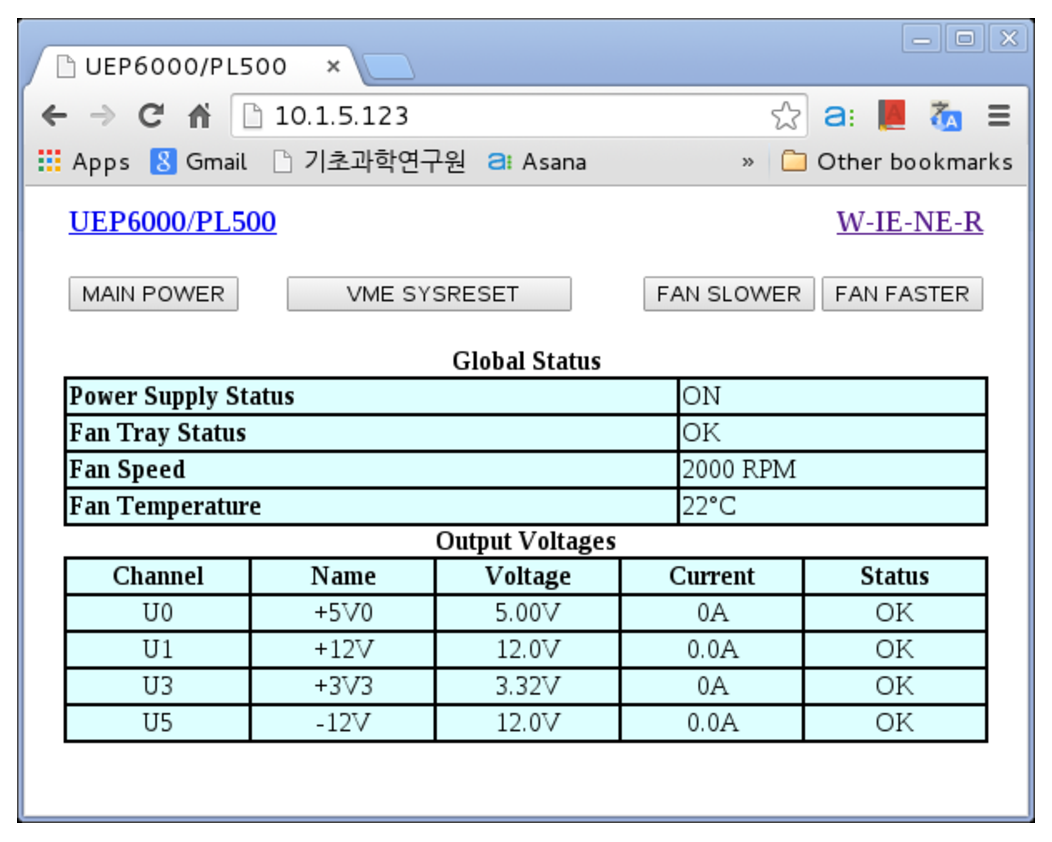
\includegraphics[width=0.45\textwidth]{./images/wienerfanr.eps}
  \label{fig:wienerwebon}   
  	    }
              \hfill
  \subbottom[WIENER Crate Fanspeed 2500]
  	    {
  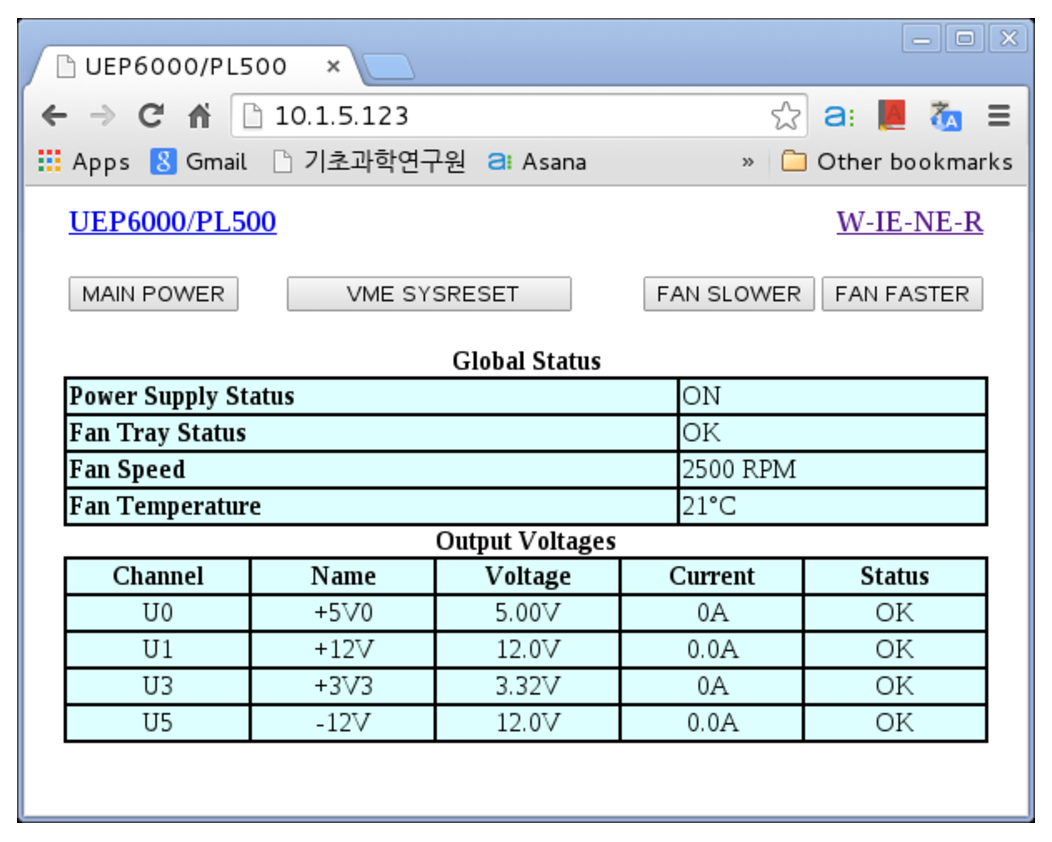
\includegraphics[width=0.45\textwidth]{./images/wienerfanw.eps}
  \label{fig:wienerweboff}   
  	    }
              \hfill
  \caption
      {
WIENER Crate webpage
      }
 \label{fig:wienerweb}
\end{figure}


위를 참조하면 모든 결과가 같으므로 EPICS IOC와 장비가 연결되어 통신함을 알 수 있다. 추가적인 장비의 정보를 레코드로 생성하고 다른 장비에 대한 Db파일을 생성해 위의 과정을 거치면 하나의 IOC에서 여러 장비의 모니터링 및 제어를 할 수 있다.


\subsection{EPICS SNMP 융합 제어 시스템 UI 개발}

CSS에서 EPICS IOC의 PV 값을 이용해 사용자가 원하는 환경에 맞춰 UI인 OPI를 구현한다.  


\subsubsection{APC Power Distribution Unit 7921}

APC사 PDU 7921의 OPI는 장비의 Power Supply, Load, Outlet의 상태를 모니터링하고 장비의 전압, Load, Outlet 등을 제어할 수 있도록 그림 \ref{fig:pduui}같이 구성한다.


\subsubsection{WIENER VME 6023 Crate }

 Wiener사의 VME64x 6023 Crate의 OPI는 그림 \ref{fig:wienerui}와 같이 Crate의 전원, 채널, 팬, 온도 센서의 상태를 모니터링하고 Power Supply와 VME의 System, 하드웨어의 reset, 팬 스피드, 온도 센서를 제어하도록 구성한다.


 \begin{figure}[!h]
   \centering
   \subbottom[APC PDU UI]
   	    {
  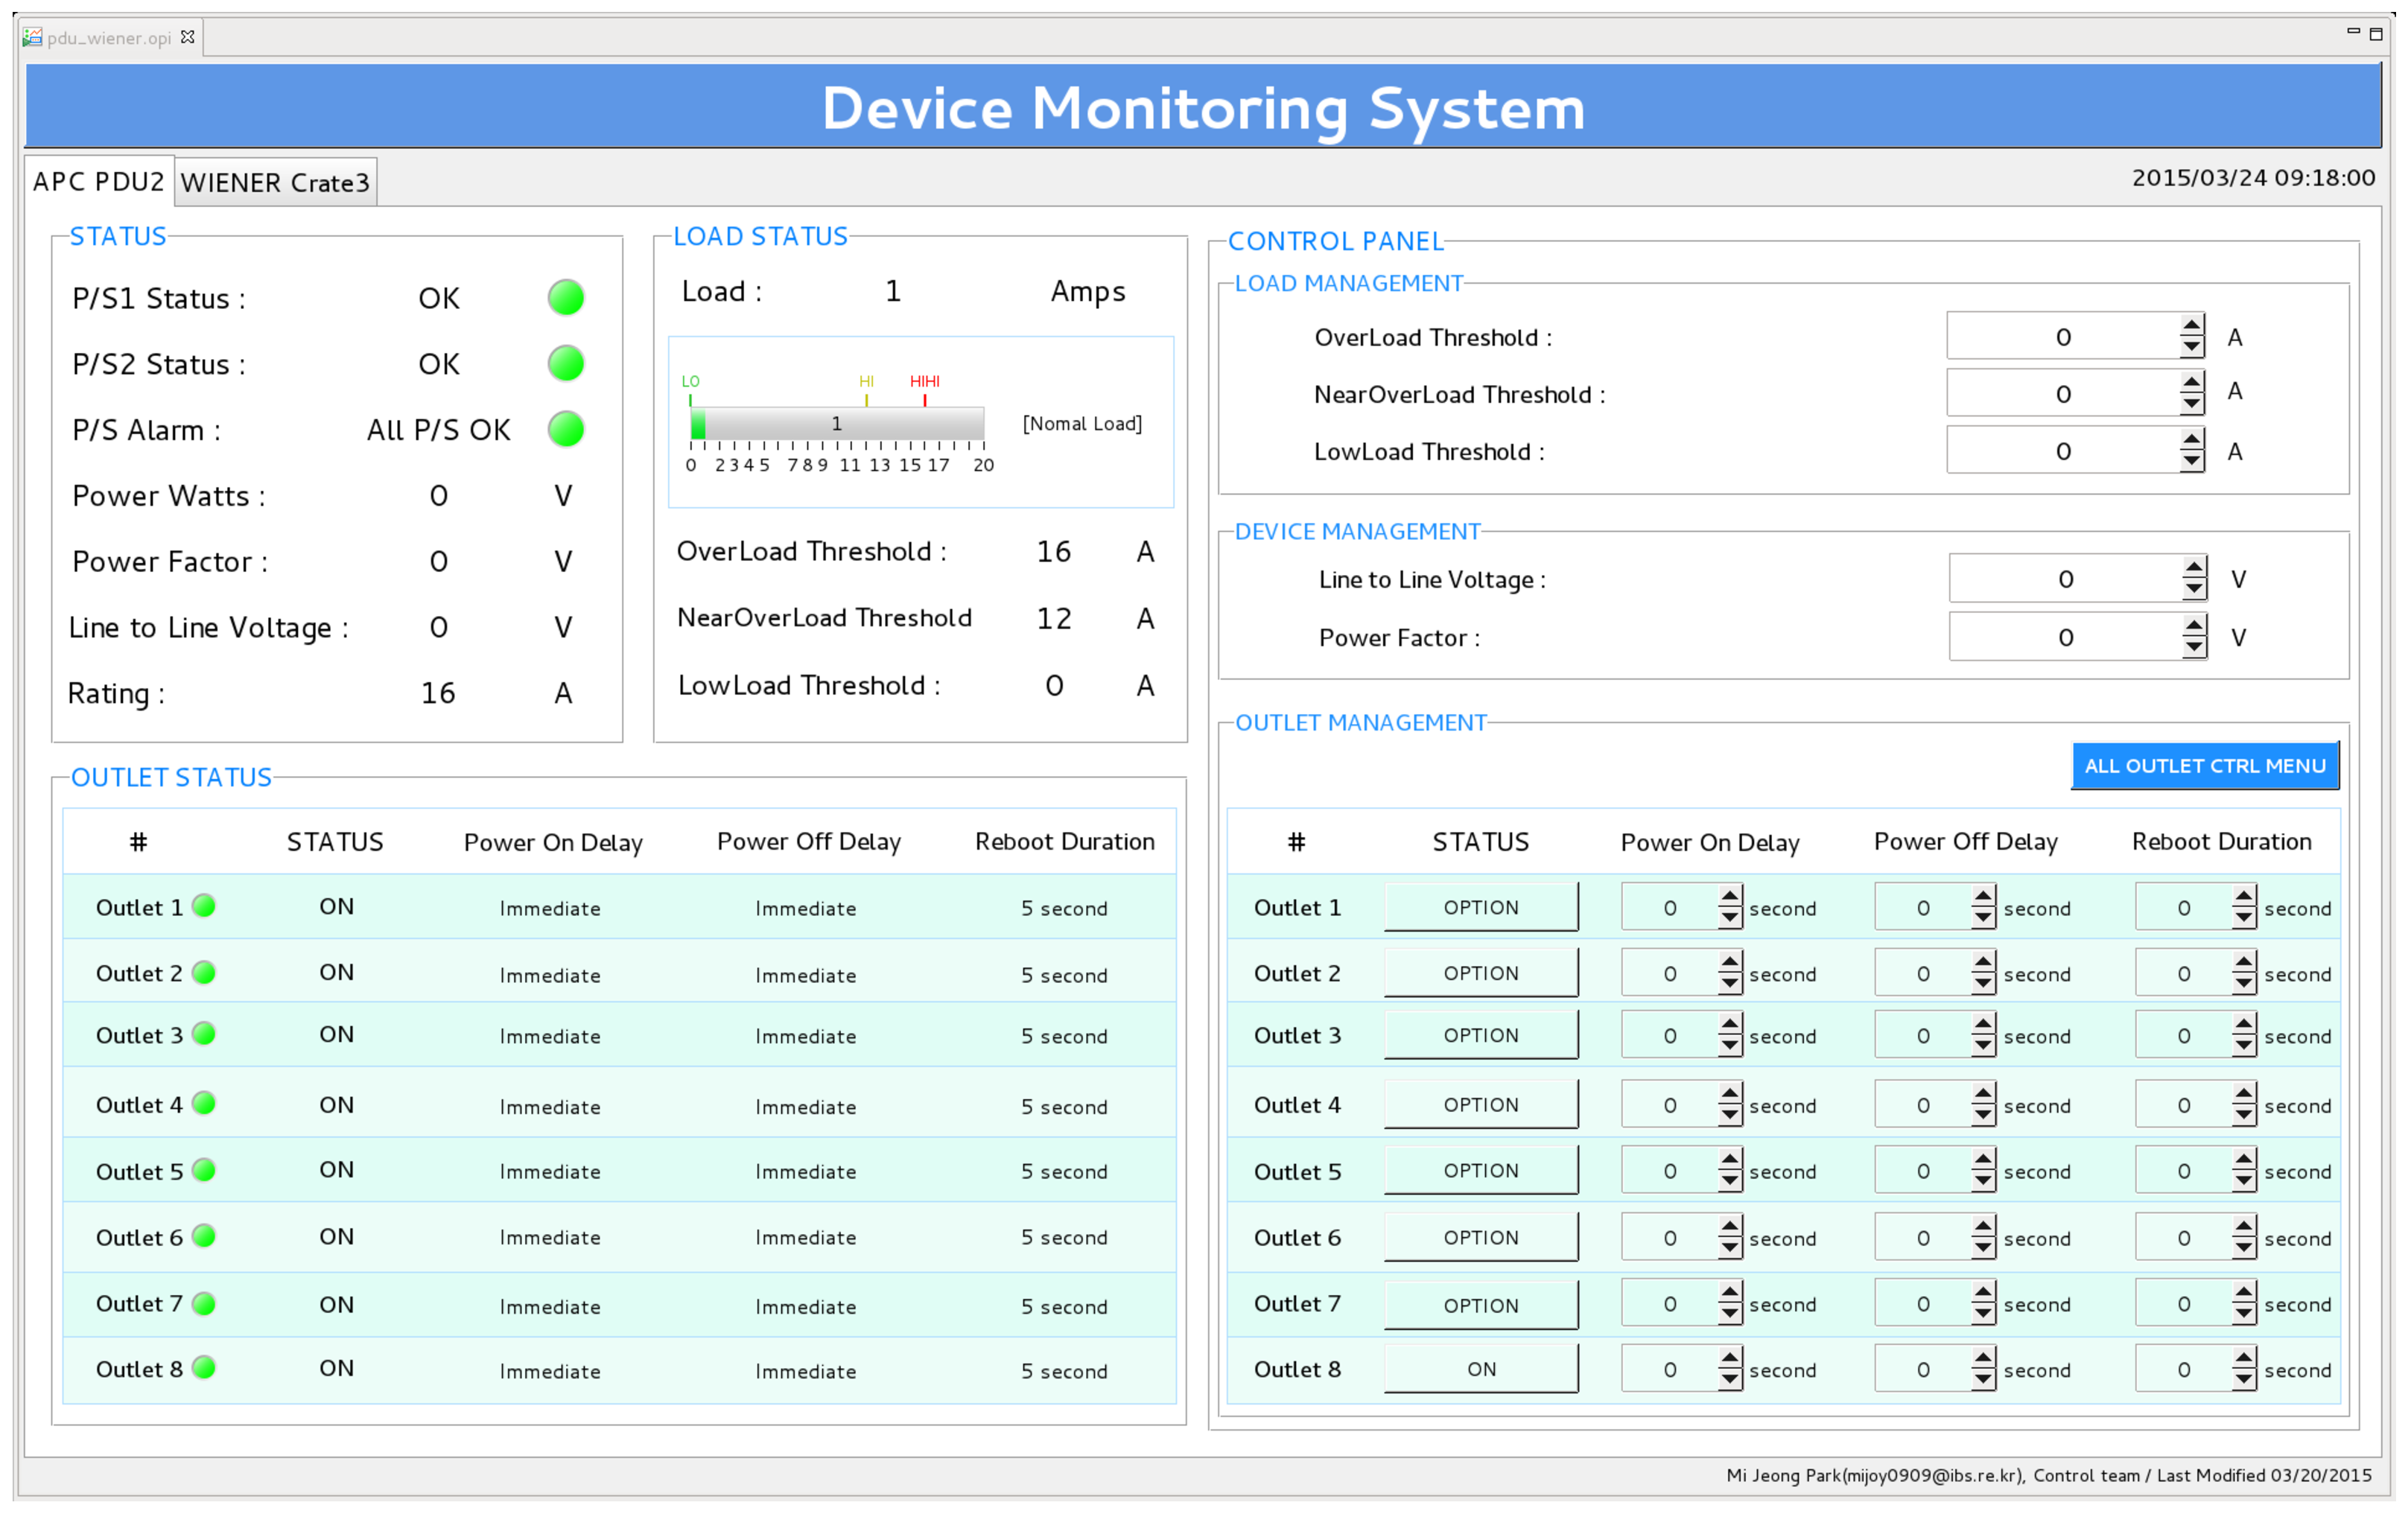
\includegraphics[width=0.7\textwidth]{./images/apcopi.eps}
  \label{fig:pduui}   
   	    }
               \hfill
   \subbottom[WIENER Crate UI]
   	    {
  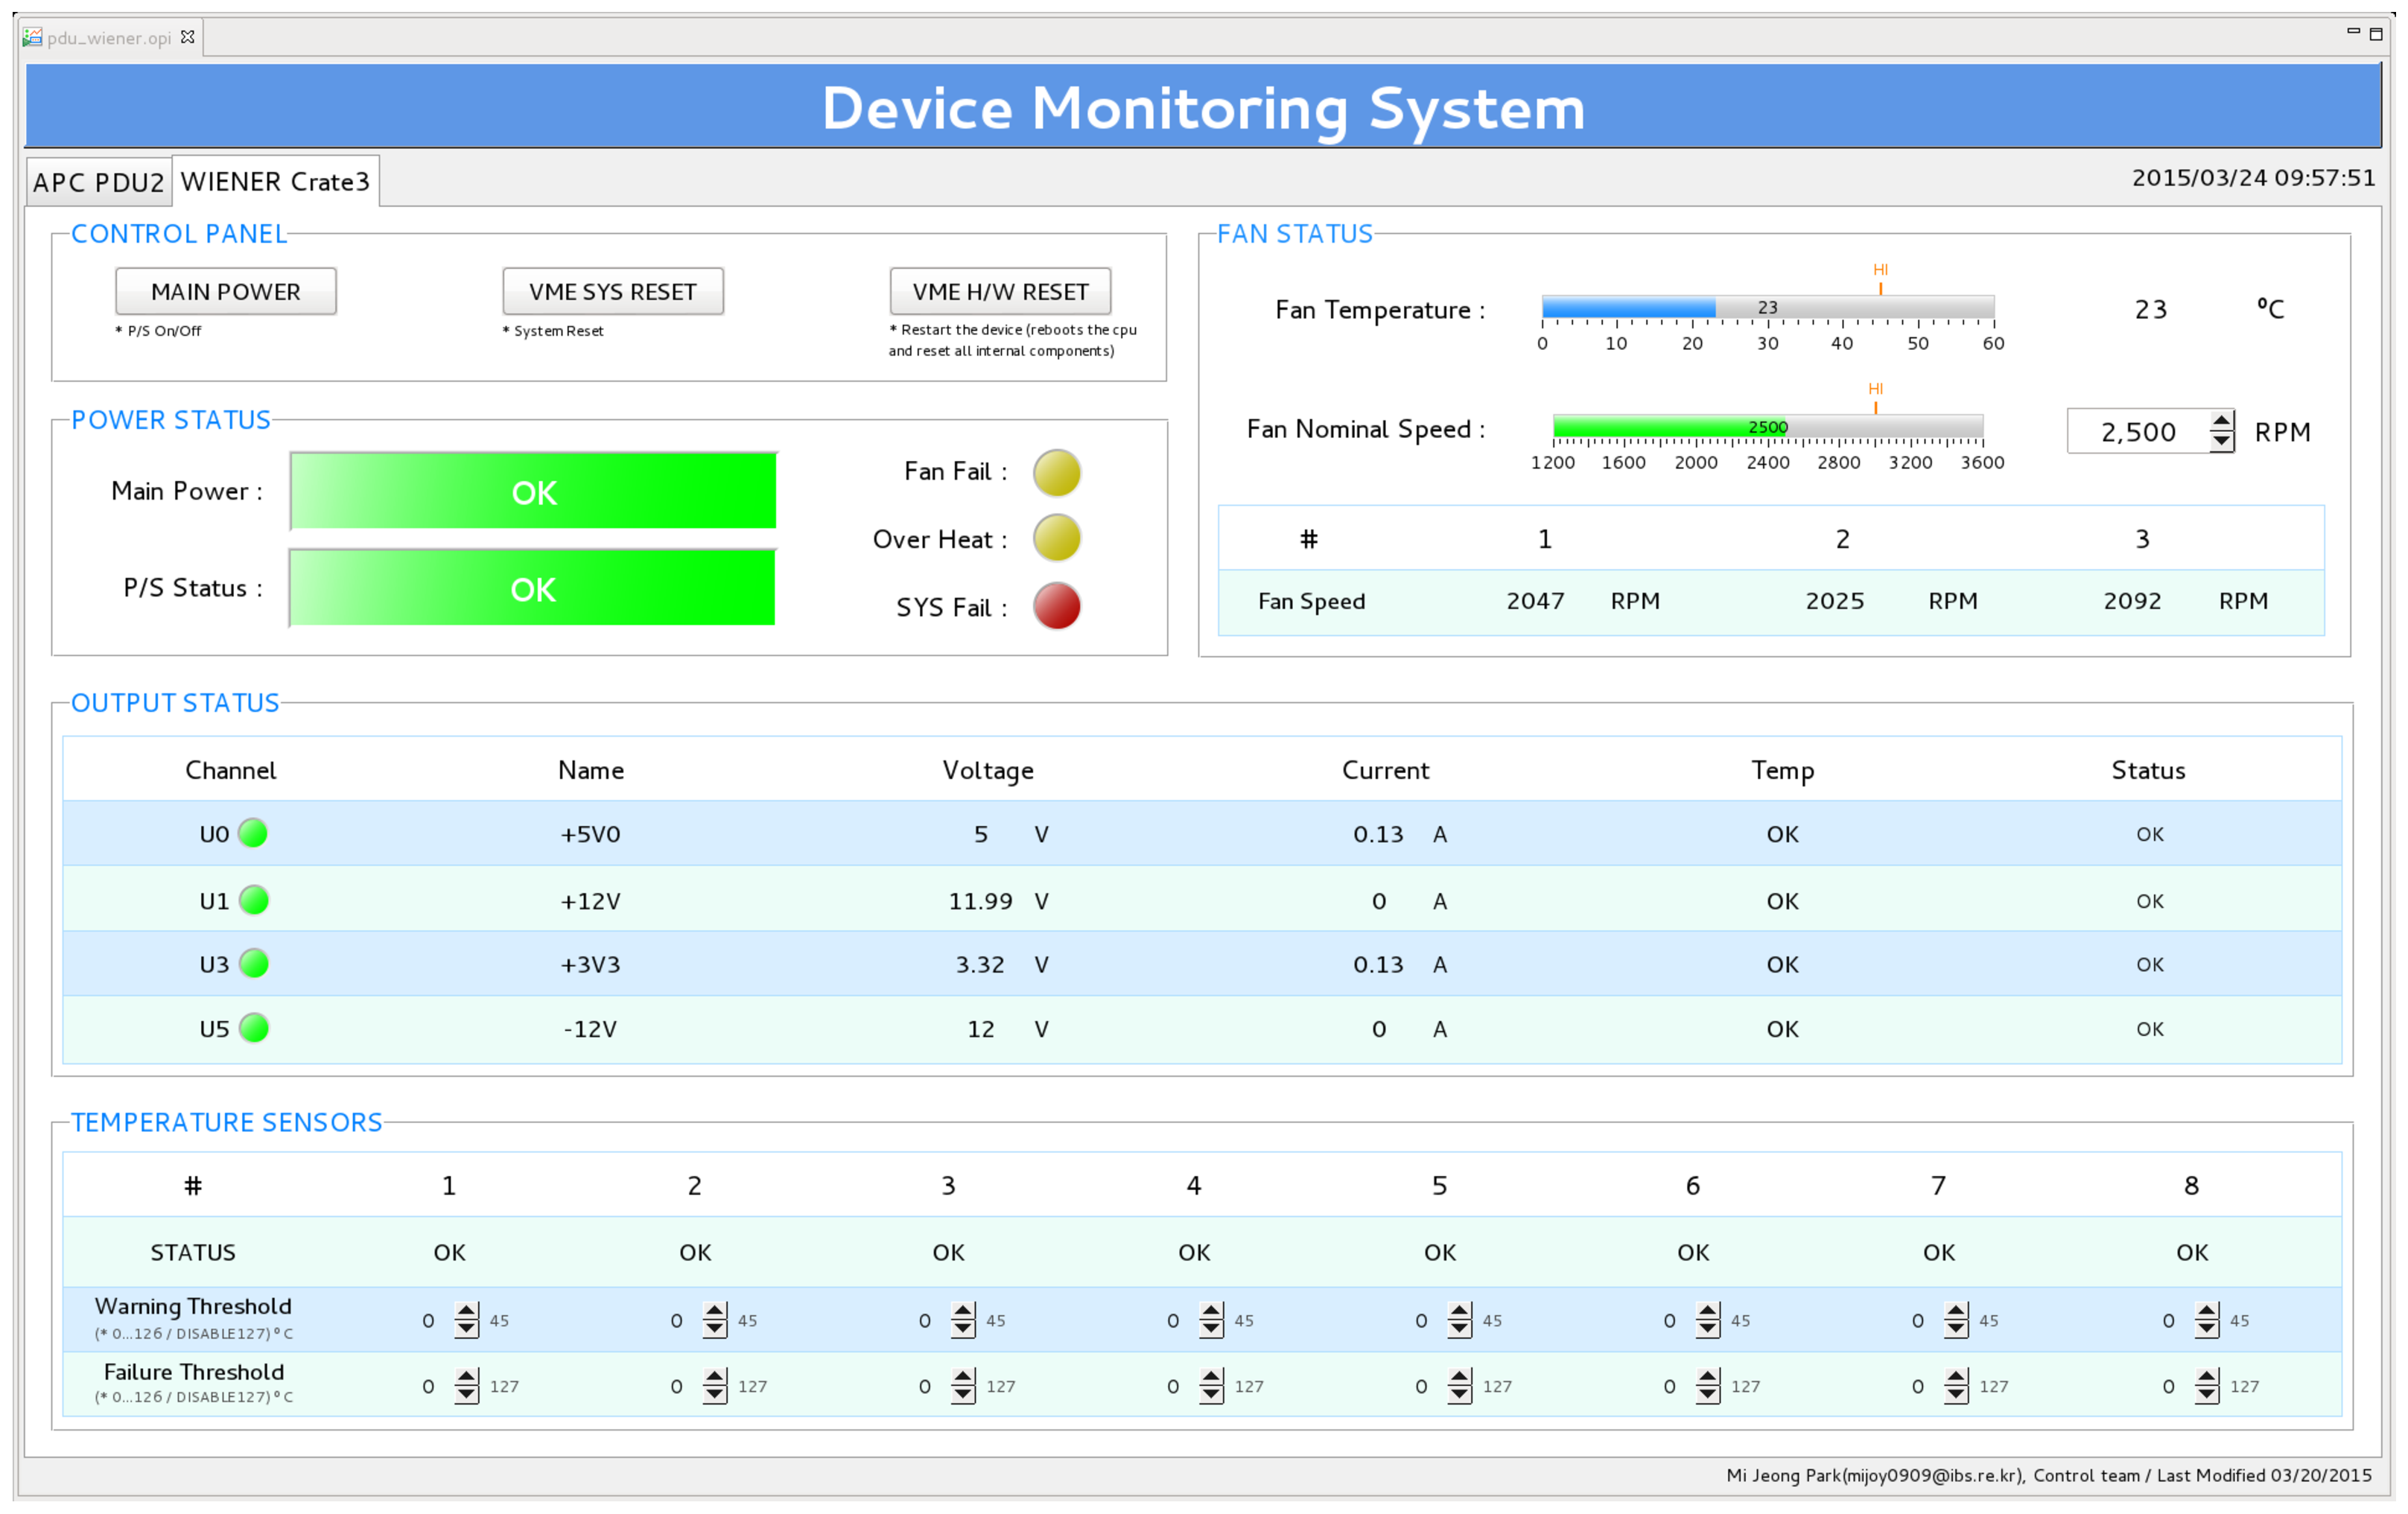
\includegraphics[width=0.7\textwidth]{./images/wienerfanw_css.eps}
  \label{fig:wienerui}   
   	    }
               \hfill
   \caption
       {
CSS를 사용해 구현한 UI
       }
  \label{fig:cssopi}
 \end{figure}

\clearpage

\section{안정성 테스트}
본 절은 완성된 융합 제어 시스템의 EPICS IOC 안정성을 테스트한다. 또한, 연구 전 SNMPv3를 지원하지 않았던 Wiener사가 본 연구의 요청으로 Crate의 SNMPv3 개발 초기 버전을 제공하였기에 Crate의 SNMP 안정성을 테스트한다. 이에 이미 산업용으로 검증된 APC사의 PDU를 함께 테스트하여 Wiener사 Crate와 안정성의 차이를 확인한다. 테스트는 Crate와 PDU의 PV 값을 주기적으로 변경하고, PV 데이터는 EPICS의 Extension툴인 Archiver Appliance를 사용해 저장 및 분석한다. 

\subsection{테스트용 Bash Script 구성}

Script는 그림\ref{fig:stability}와 같이 구성된다. 이는 특정 시간을 주기로 Wiener사의 Crate의 팬 스피드를 100단위로 1200에서 3600까지 올렸다, 내리고 APC사의 PDU Outlet 8번의 전원을 켰다 끈다. 이때 SNMP 명령어와 camonitor로 통신 되는 값을 모두 확인하고 Script의 결과는 아래와 같은 형식의 로그 파일로 저장된다. 자세한 Script는 부록을 참조 바란다.

\begin{figure}[h!]
  \centering
  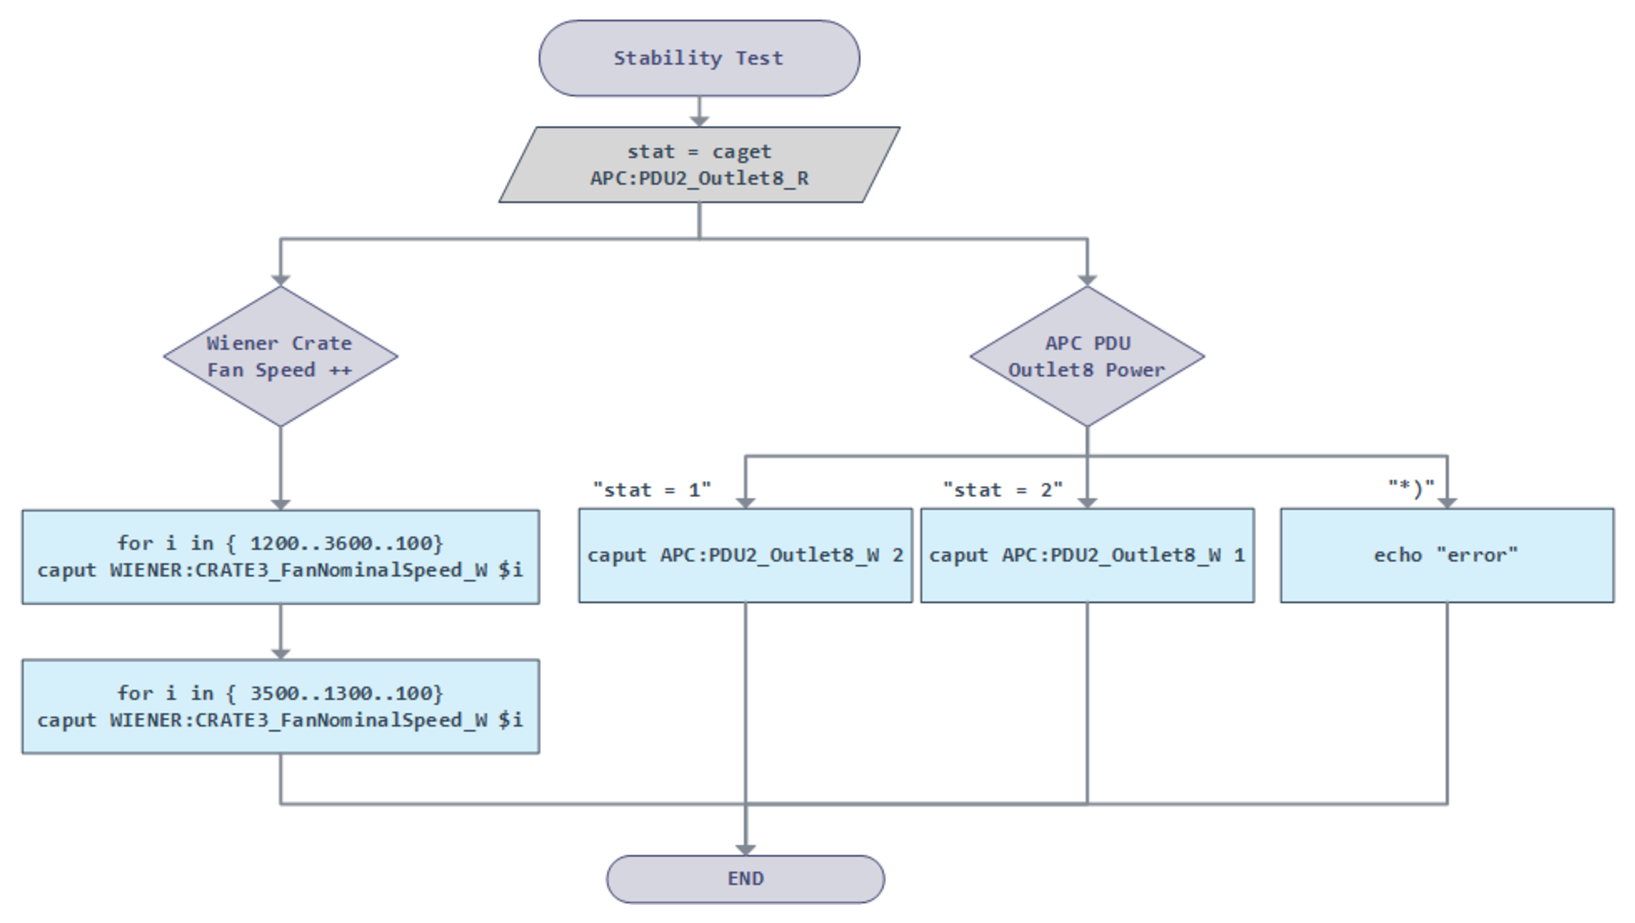
\includegraphics[width=0.89\textwidth]{./images/stability.eps}
  \caption{안정성 테스트 Script 순서도}
  \label{fig:stability}   
\end{figure}

\begin{lstlisting}[style=termstyle]
***************************************************************
SNMPIOC:TIMESTAMP              2015/03/24 19:07:23
---------------------------------------------------------------
snmpget -------------------------------------------------------
WIENER-CRATE-MIB::sysMainSwitch.0 = INTEGER: ON(1)
WIENER-CRATE-MIB::sysStatus.0 = BITS: 80 mainOn(0) 
WIENER-CRATE-MIB::fanAirTemperature.0 = INTEGER: 22 \ufffdC
WIENER-CRATE-MIB::fanNominalSpeed.0 = INTEGER: 2400 RPM
PowerNet-MIB::sPDUOutletCtl.8 = INTEGER: outletOn(1)
---------------------------------------------------------------
caget ---------------------------------------------------------
WIENER:CRATE3_MainPower_R      1
WIENER:CRATE3_PS_Status        80 mainOn(0)
WIENER:CRATE3_FanairTemp       22
WIENER:CRATE3_FanNominalSpeed_R 2400
WIENER:CRATE3_FanNominalSpeed_W 2400
APC:PDU2_Outlet8_R             1
APC:PDU2_Outlet8_W             1
caput ---------------------------------------------------------
Old : APC:PDU2_Outlet8_W             1
New : APC:PDU2_Outlet8_W             2
Old : WIENER:CRATE3_FanNominalSpeed_W 2400
New : WIENER:CRATE3_FanNominalSpeed_W 2500
\end{lstlisting}

\subsection{Raspberry Pi를 활용한 모니터링}
스크립트가 실행될 때 변경되는 PV 값이 실제 Crate의 팬 스피드에 영향을 미치는지 확인하기 위해 Wiener사에서 제공하는 웹페이지와 Raspberry Pi의 카메라 모듈을 활용하여 그림 \ref{fig:rpimonitoring}과 같이 Crate의 패널을 모니터링한다.

\begin{figure}[!h]
  \centering
  \subbottom[Raspberry Pi Camera Module]
  	    {
  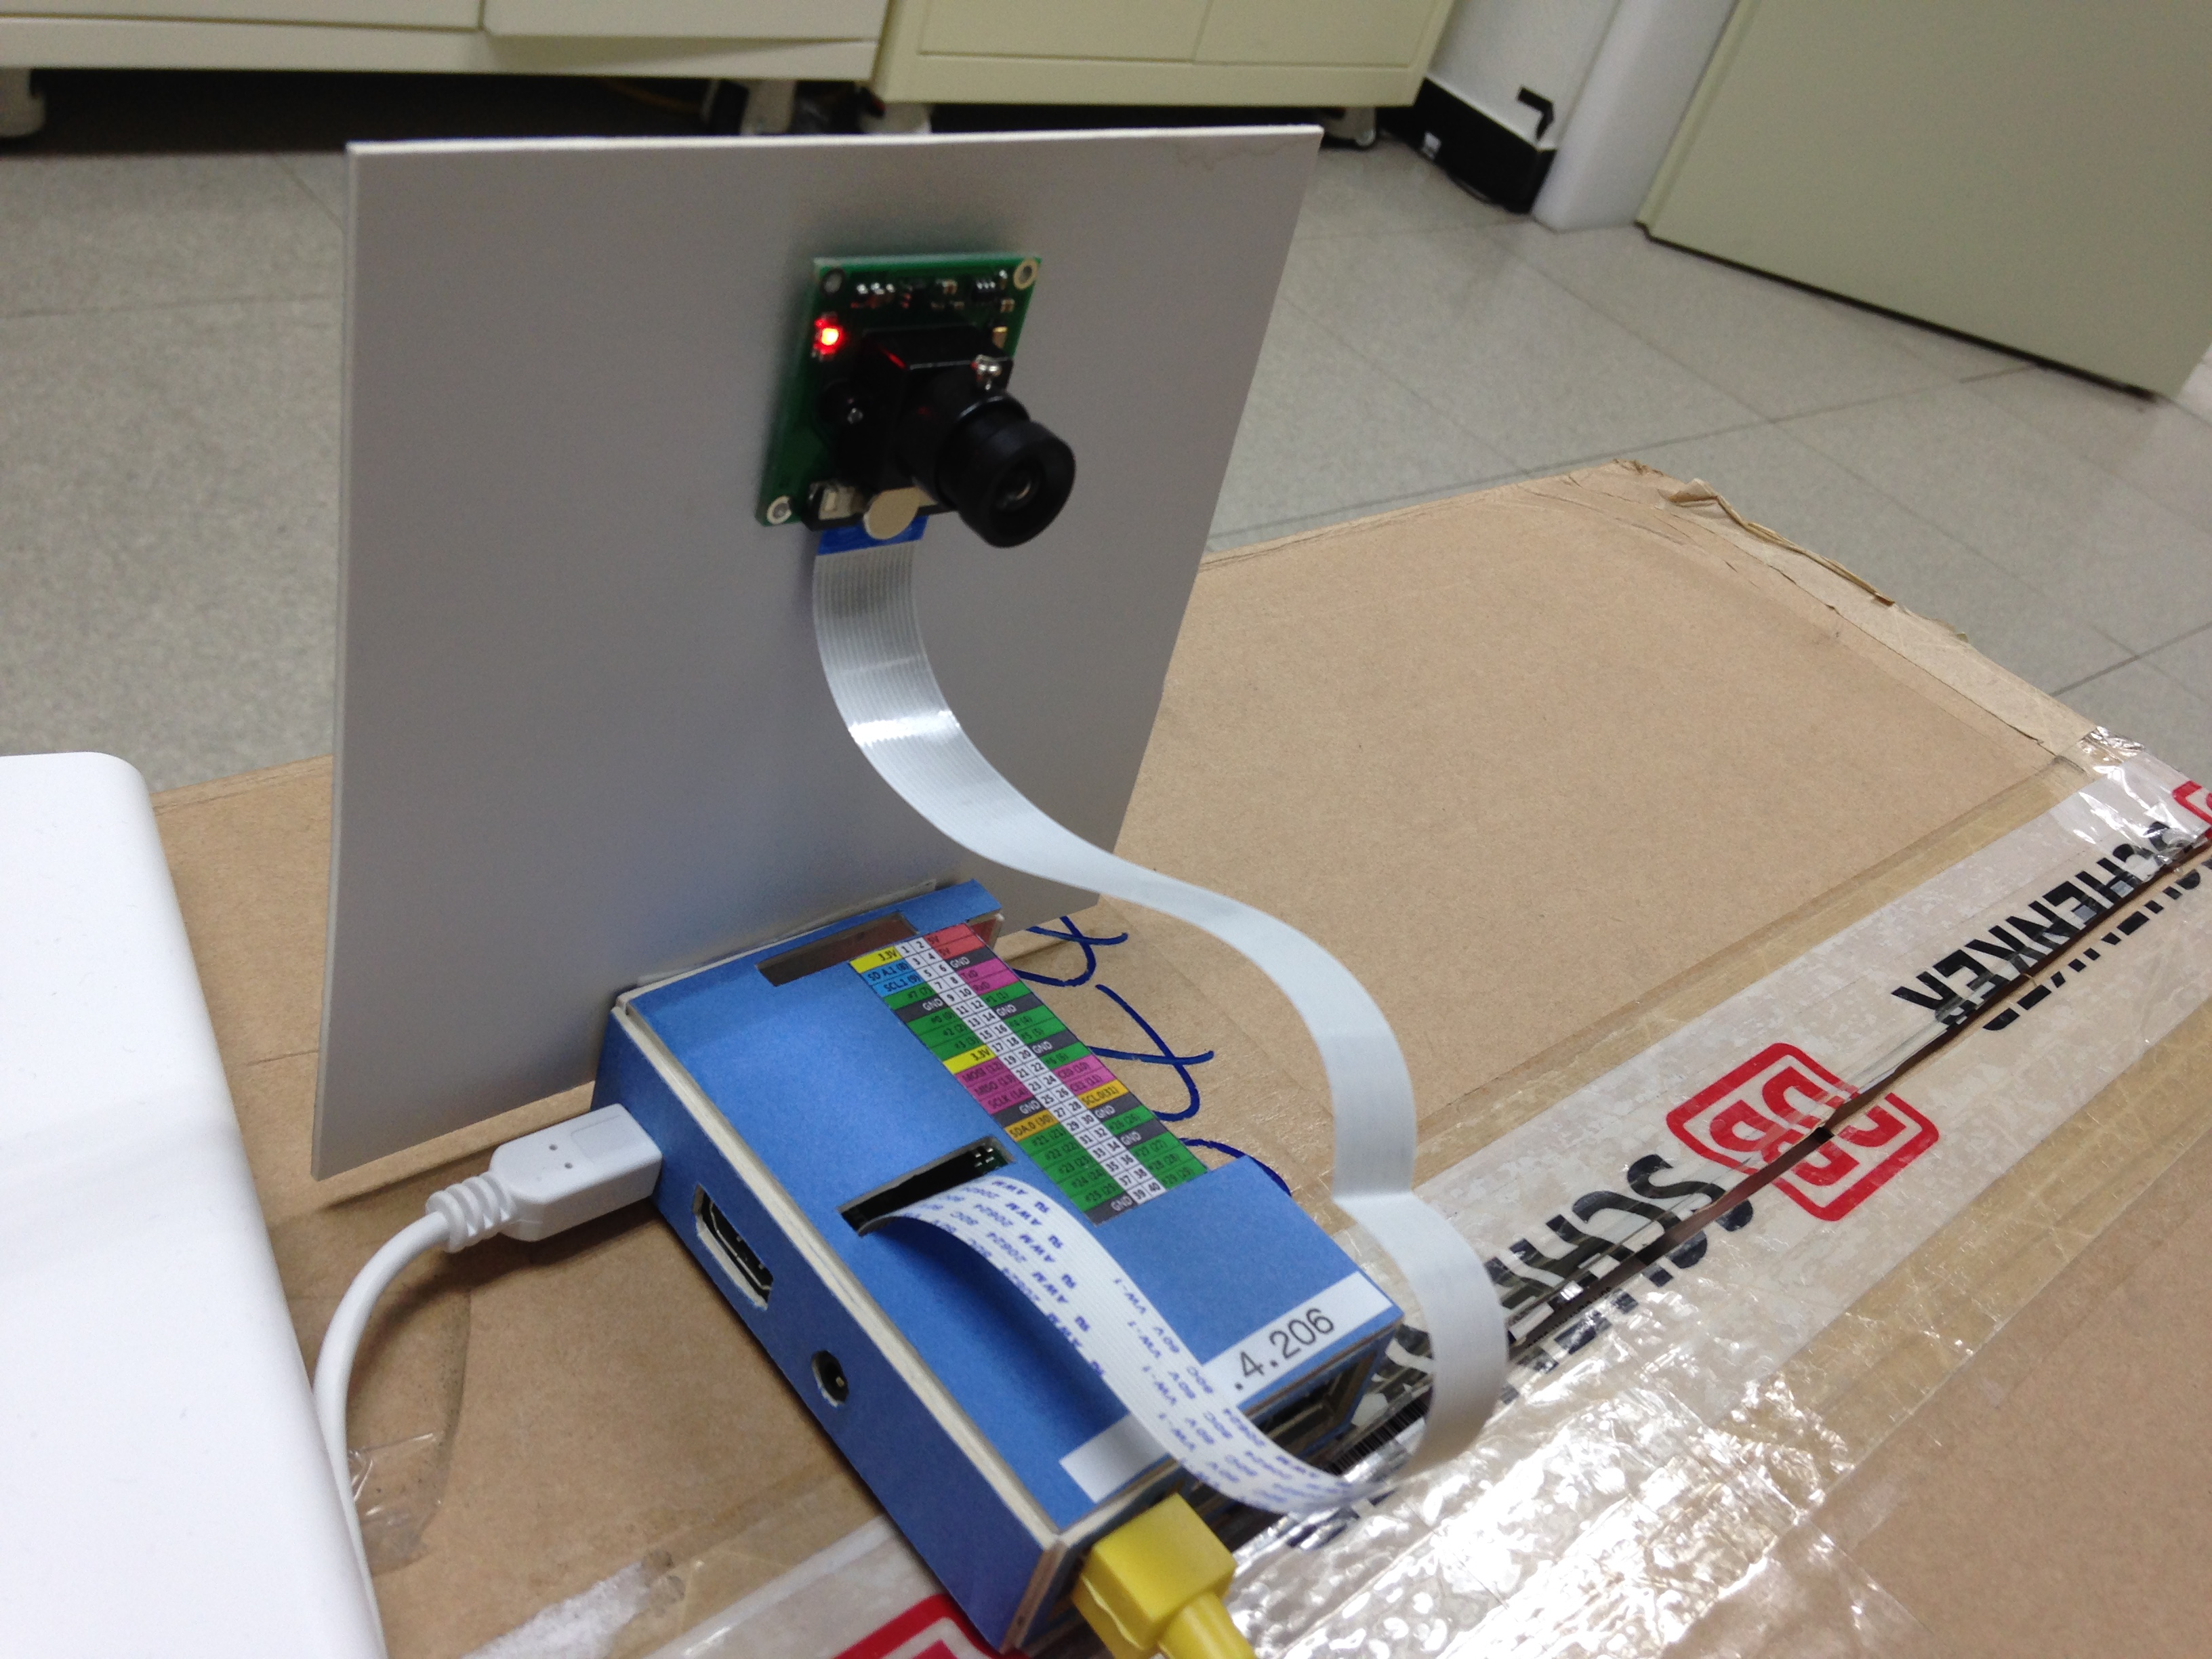
\includegraphics[width=0.45\textwidth]{./images/Rpi.eps}
  \label{fig:rpi}   
  	    }
              \hfill
  \subbottom[Raspberry Pi Monitoring Environment]
  	    {
  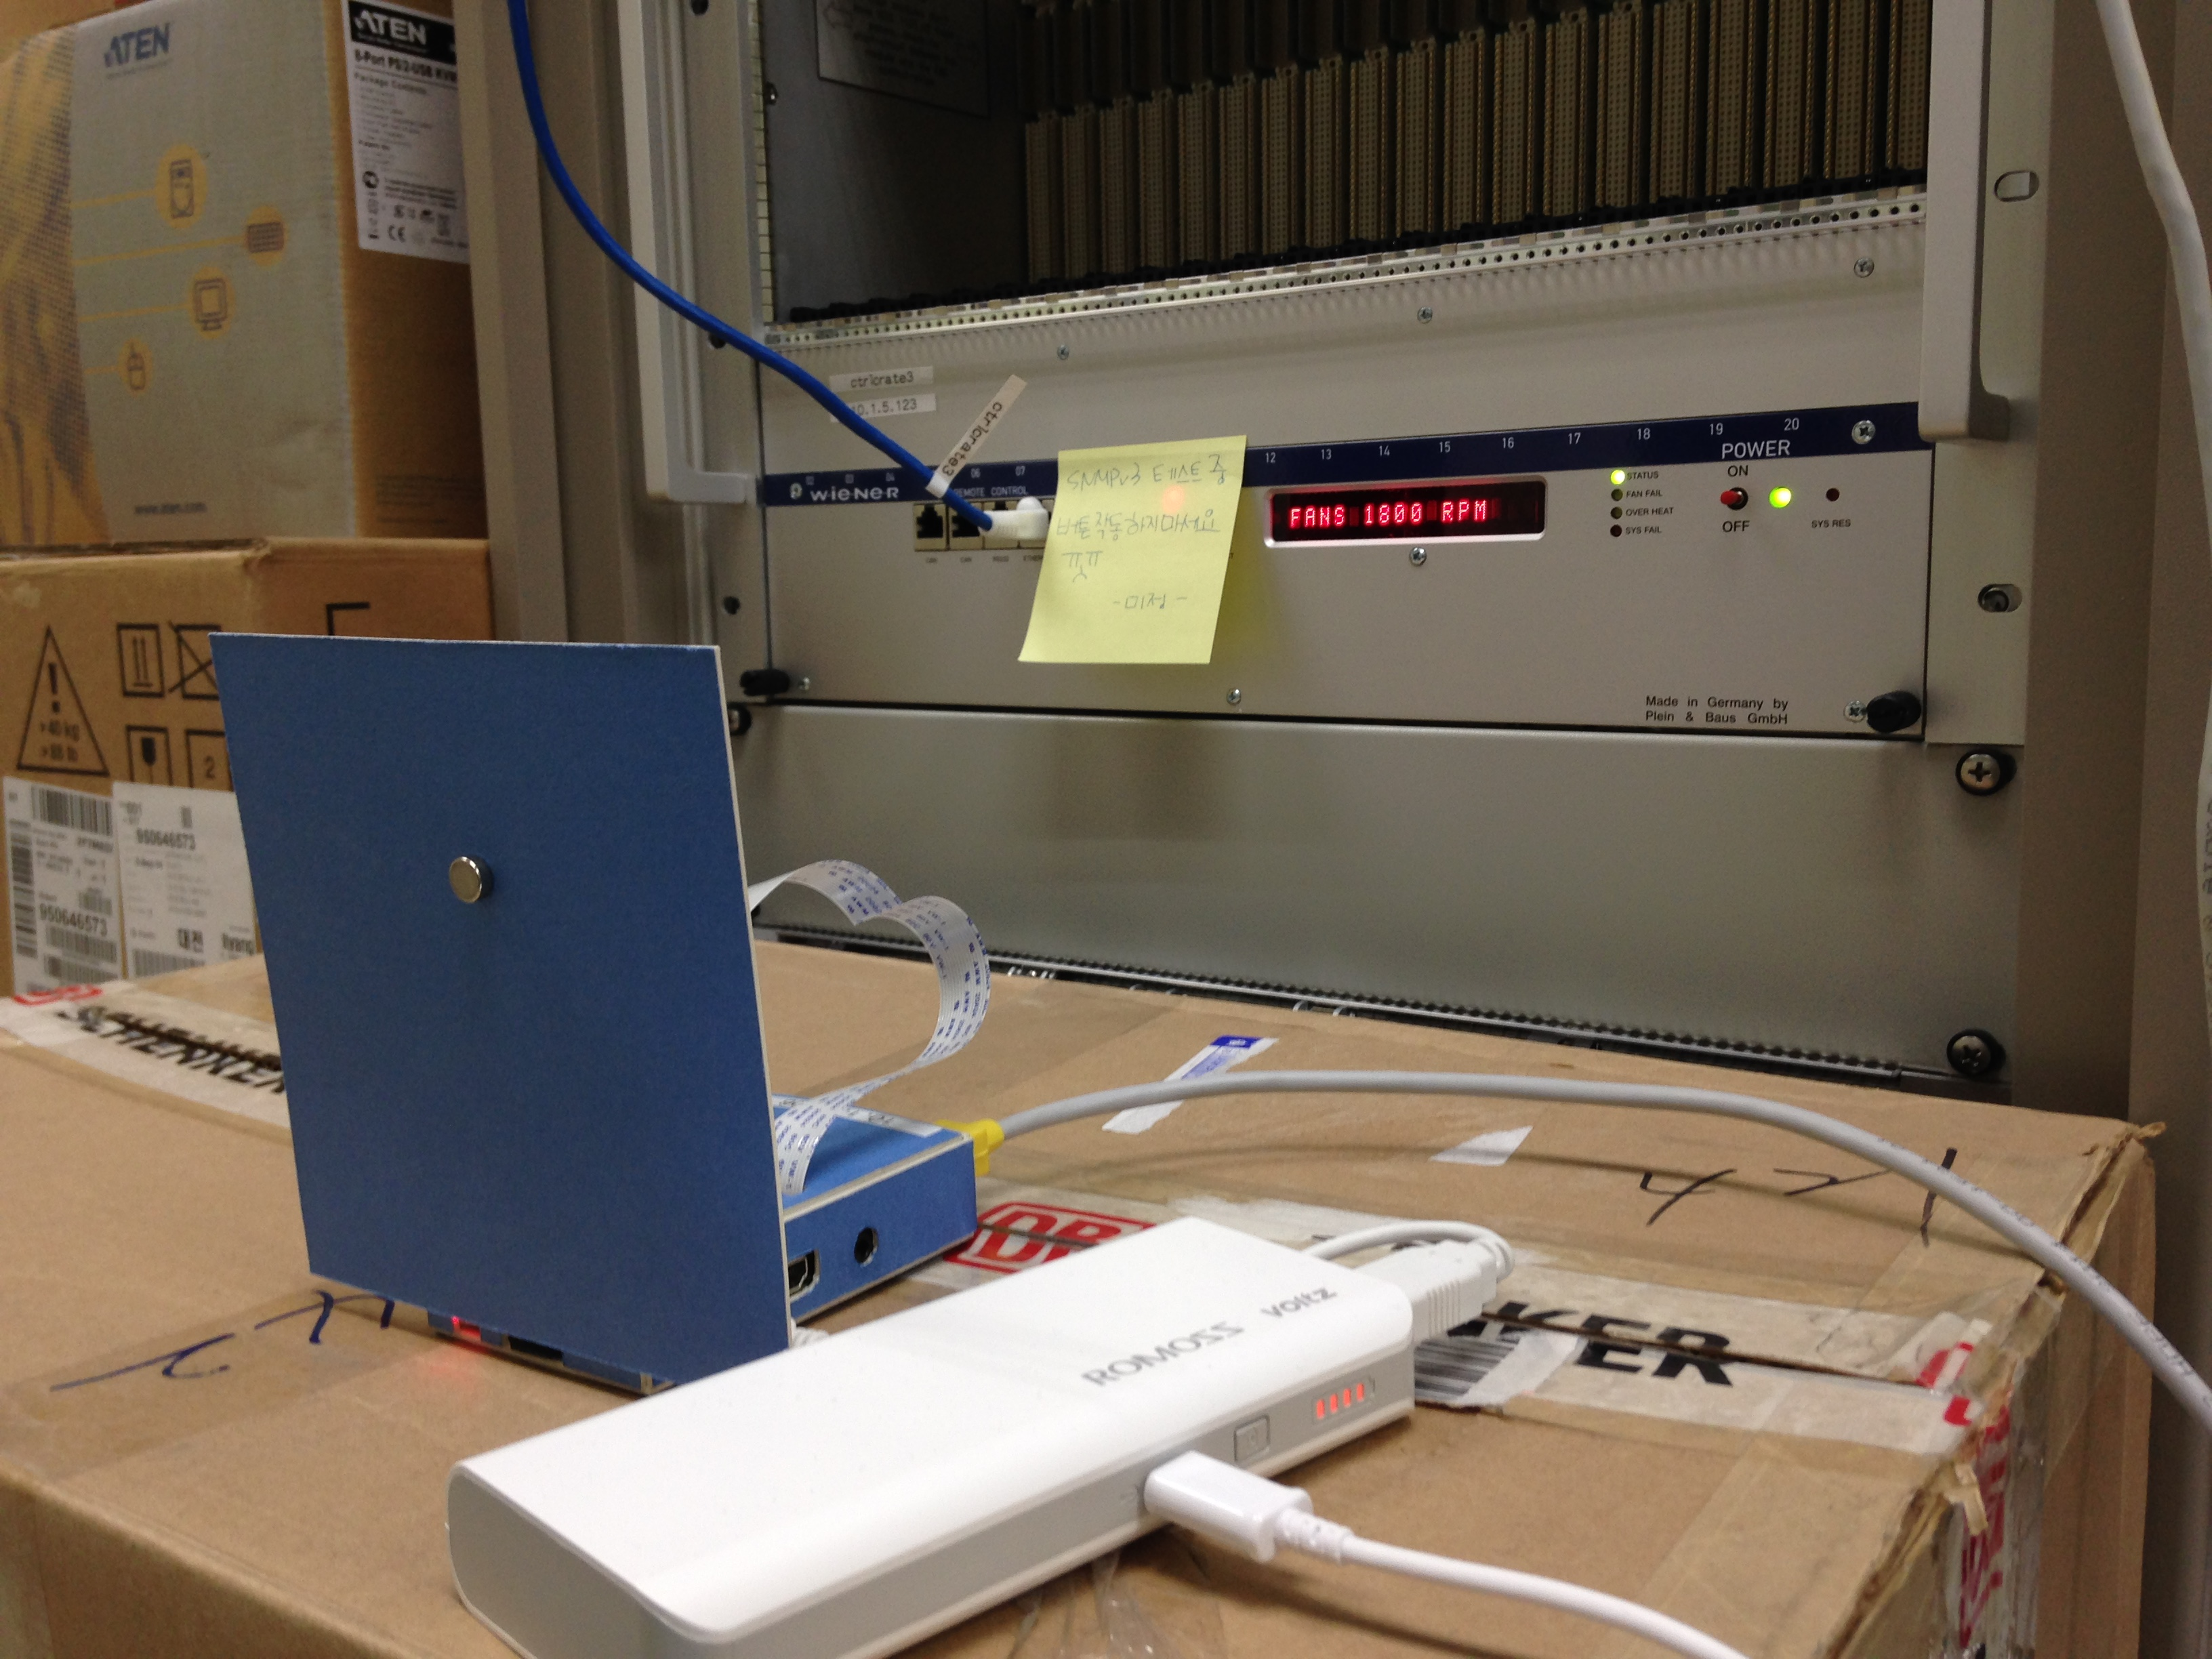
\includegraphics[width=0.45\textwidth]{./images/Rpitest.eps}
  \label{fig:rpitest}   
  	    }
              \hfill
  \caption
      {
Monitoring using Raspberry Pi Camera
      }
 \label{fig:rpimonitoring}
\end{figure}

카메라 모듈로 촬영되는 영상은 mjpg streamer Library를 사용하면 Web Streaming을 통해 그림 \ref{fig:javapage}과 같이 웹페이지로 볼 수 있다. 

\begin{figure}[h!]
  \centering
  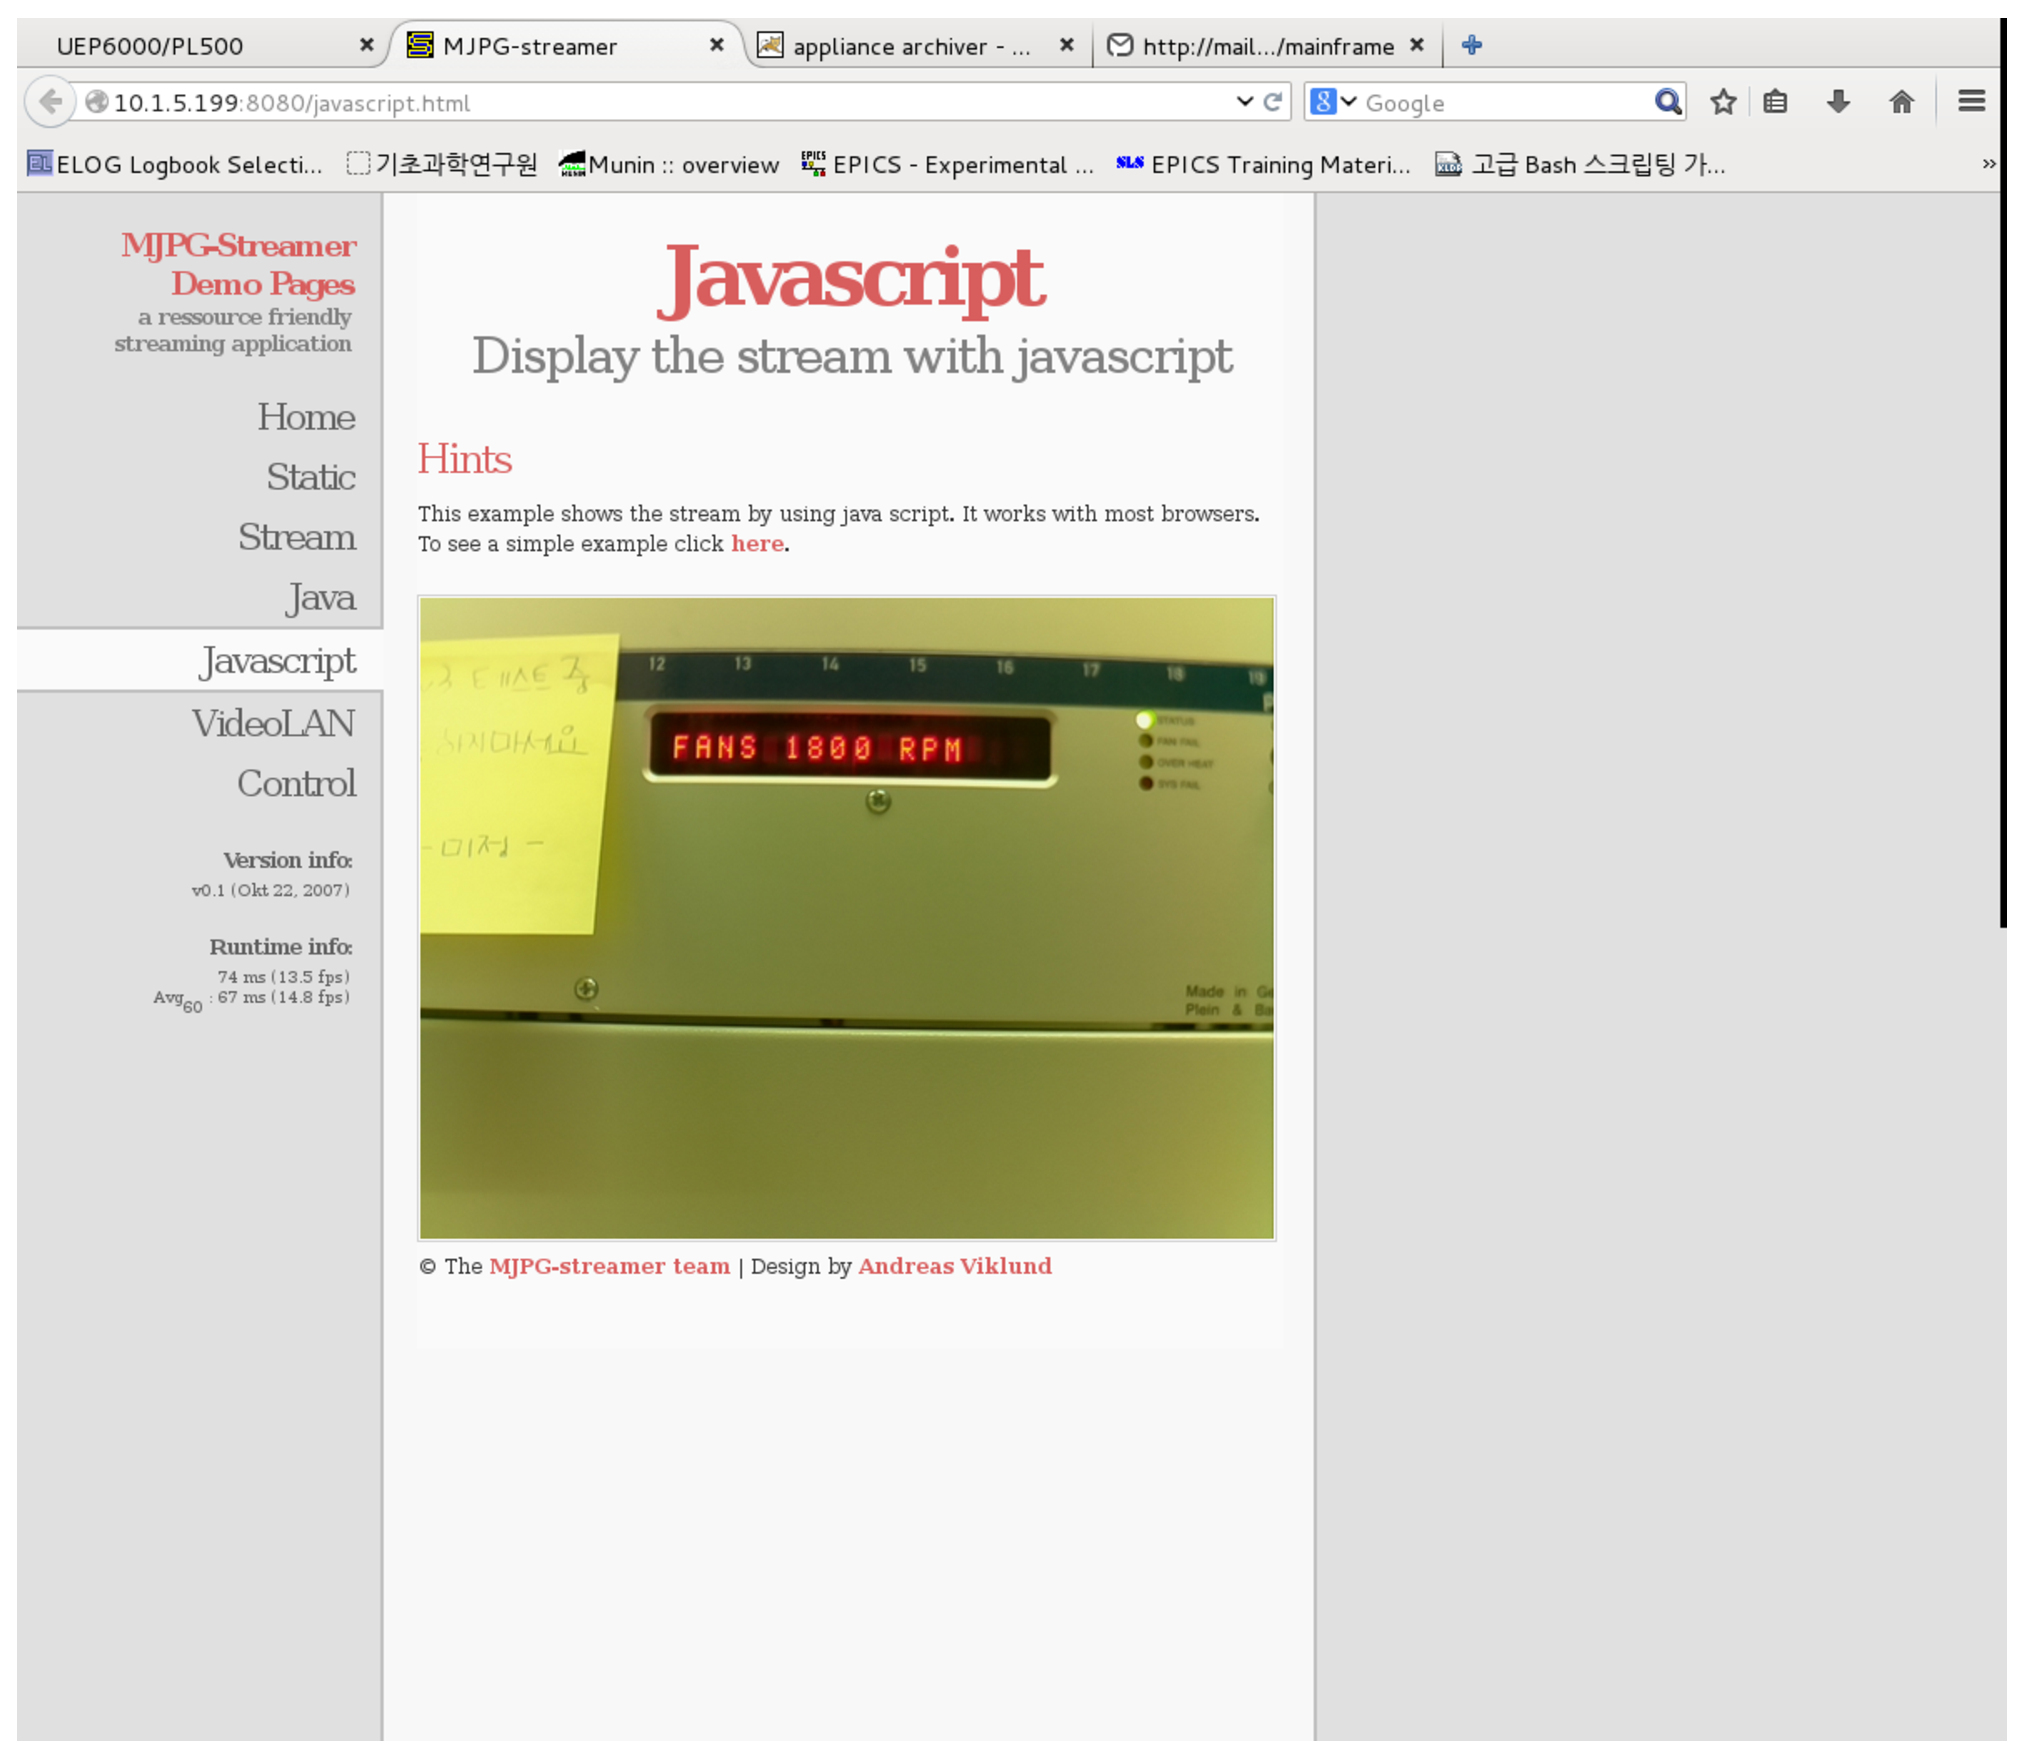
\includegraphics[width=0.68\textwidth]{./images/javapage.eps}
  \caption{R.pi 카메라 모듈 모니터링 페이지}
  \label{fig:javapage}   
\end{figure}

\clearpage


\subsection{Archiver Appliance}
Archiver Appliance는 SLAC에서 개발된 Engine, Retrieval, ELT (Extraction, Transformation, Load), MGMT (Management)의 4개 모듈로 구성되고, Java언어로 개발 된 EPICS 데이터 저장 유틸리티이다. MGMT 모듈을 사용해 표 \ref{table:pvlist}의 PV리스트를 그림 \ref{fig:archiver}과 같이 입력해 Archive 버튼을 눌러 데이터 저장을 시작한다. 

\begin{figure}[h!]
  \centering
  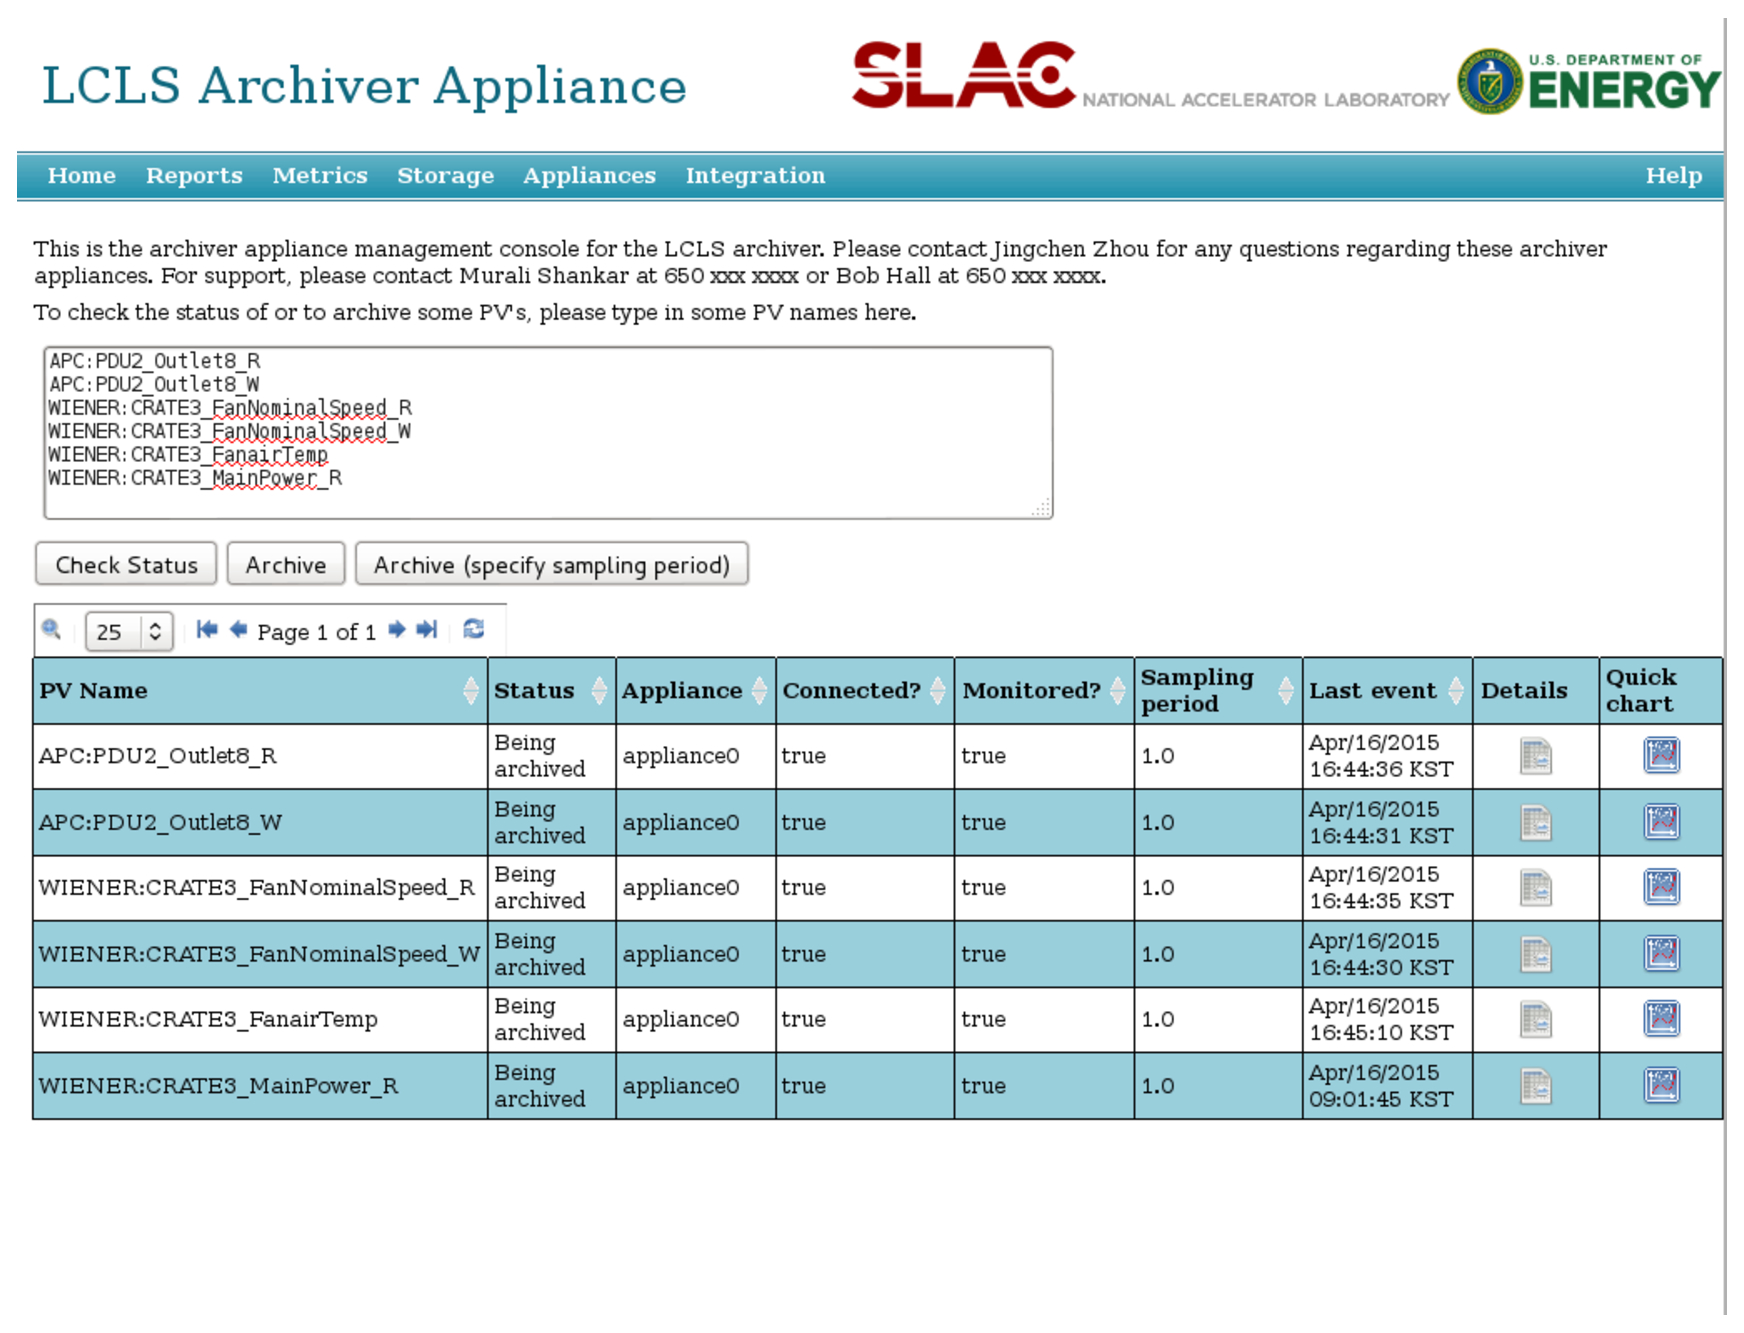
\includegraphics[width=0.68\textwidth]{./images/aaa.eps}
  \caption{Archiver Appliance List Box}
  \label{fig:archiver}   
\end{figure}



\begin{table}[h!]
\begin{center}
\small 
\begin{tabulary}{\textwidth}{C|C|C}
PV Name& Comments & Version\\ \hline
\$\{A\}:\$\{P\}\_Outlet8\_R & Outlet 8번 상태 Read  & v2c\\ 
& (On : 1/Off : 2/Reboot : 3) & \\ \hline
\$\{A\}:\$\{P\}\_Outlet8\_W & Outlet 8번 상태 Write & v3\\
& (On : 1/Off : 2/Reboot : 3) & \\ \hline
\$\{W\}:\$\{C\}\_FanNominalSpeed\_R & 팬 스피드 Read & v2c\\ \hline
\$\{W\}:\$\{C\}\_FanNominalSpeed\_W & 팬 스피드 Write & v3\\ \hline
\$\{W\}:\$\{C\}\_FanairTemp & 팬 온도 Read & v2c\\ \hline
\$\{W\}:\$\{C\}\_MainPower\_R & Crate Main Power 상태 Read & v2c \\ 
& (On : 1/Off : 0)& \\
\end{tabulary}
\caption{안정성 테스트에 사용된 PV와 SNMP 버전 (R:Read/W:Write)  }{* \$\{A\}:\$\{P\}\_는 APC:PDU2} \\{* \$\{W\}:\$\{C\}\_는 WIENER:CRATE3}
  \label{table:pvlist} 
\end{center}
\end{table} 

저장되는 PDU Outlet 8번의 전원 On/Off, Wiener Crate의 팬 스피드, 온도, Power 대한 데이터를 ArchiverViewer을 통해 그림 \ref{fig:aaviewer}과 같이 확인하면서 융합 제어 시스템의 안정성을 테스트하였다. 
 
\begin{figure}[h!]
  \centering
  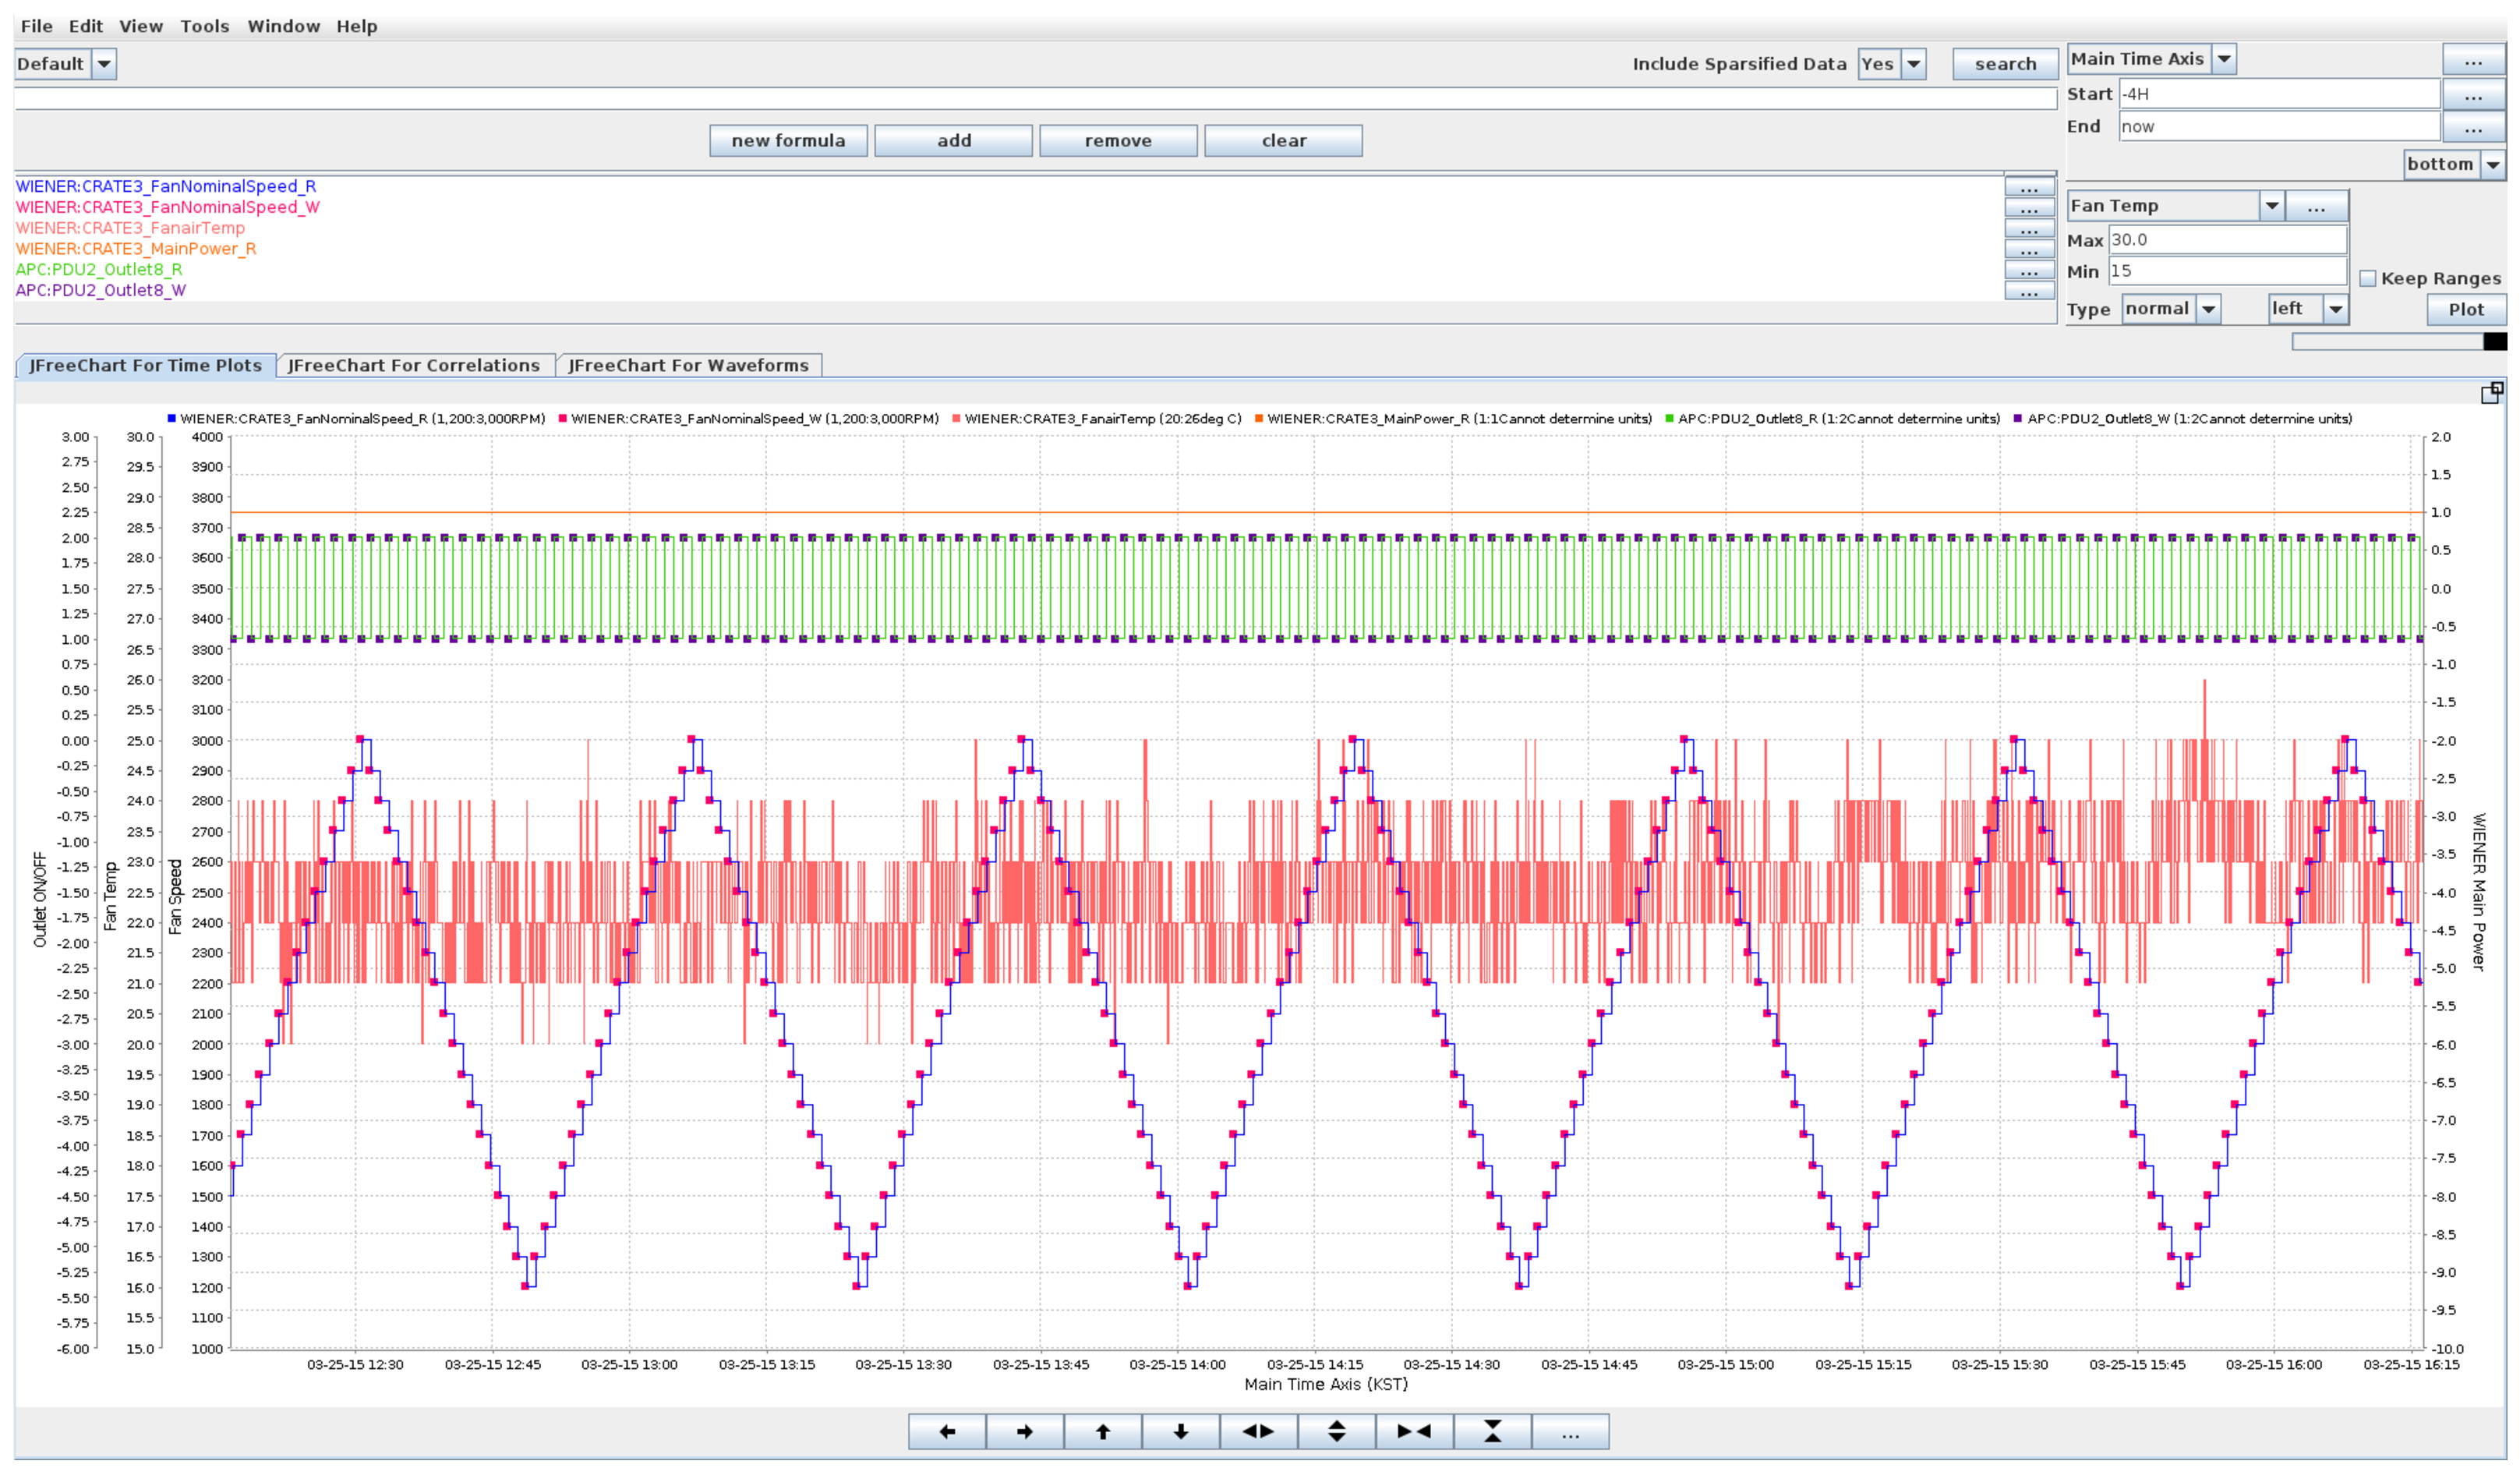
\includegraphics[width=0.99\textwidth]{./images/aaviewer_3.eps}
  \caption{Archiver Appliance Viewer}
  \label{fig:aaviewer}   
\end{figure}

\subsection{테스트 결과}

\subsubsection{EPICS IOC의 안정성}
SNMP API를 활용하여 만든 EPICS IOC가 제대로 동작하는지 확인하기 위해 APC사의 PDU를 사용하였다. 그림 \ref{fig:outlet}와 같이 PDU의 Outlet 8번의 Read (SNMPv2c)/Write(SNMPv3) PV는 한 달 동안 문제없이 동작하였음을 알 수 있다. 또한 그림 \ref{fig:wienerv3}의 Wiener사 Crate의 Read(SNMPv2c)를 사용한 팬의 온도와 전원에 대한 PV 역시 문제가 없음을 알 수 있다.


\begin{figure}[h!]
  \centering
  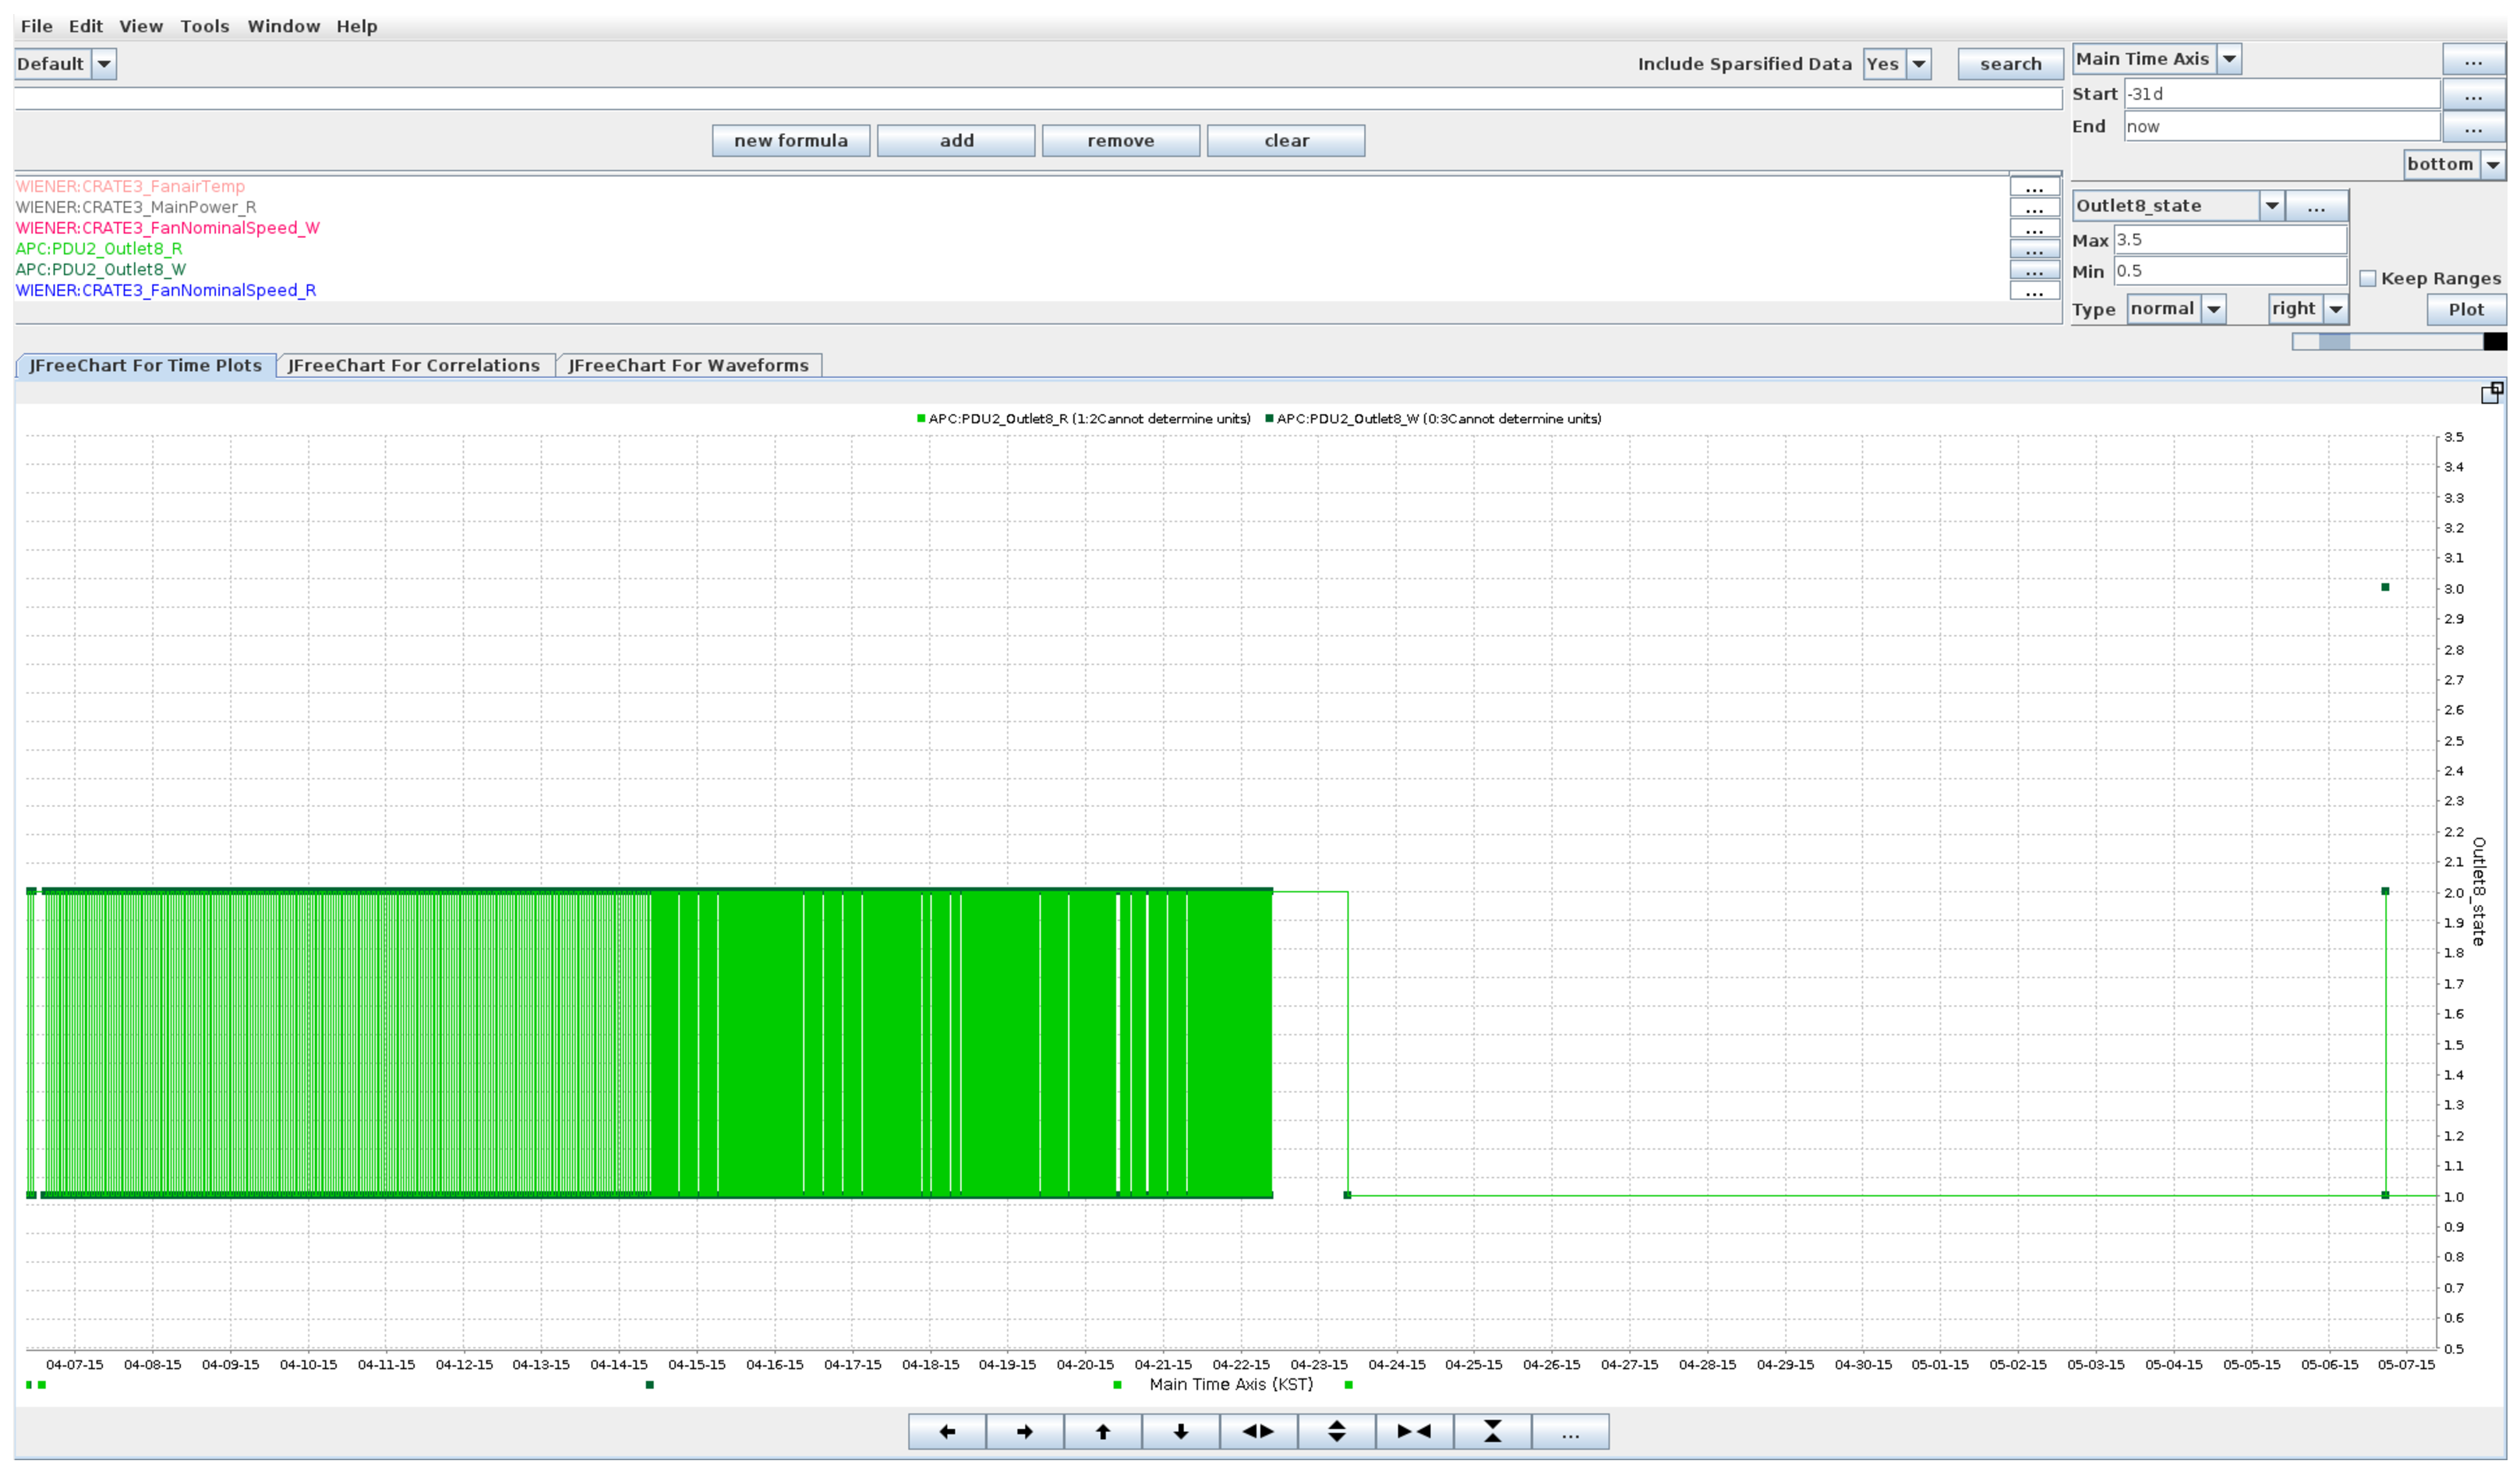
\includegraphics[width=0.99\textwidth]{./images/0507_archiver_wiener_outlet8_2.eps}
  \caption{Archiver Appliance Viewer}
  \label{fig:outlet}   
\end{figure}

\begin{figure}[h!]
  \centering
  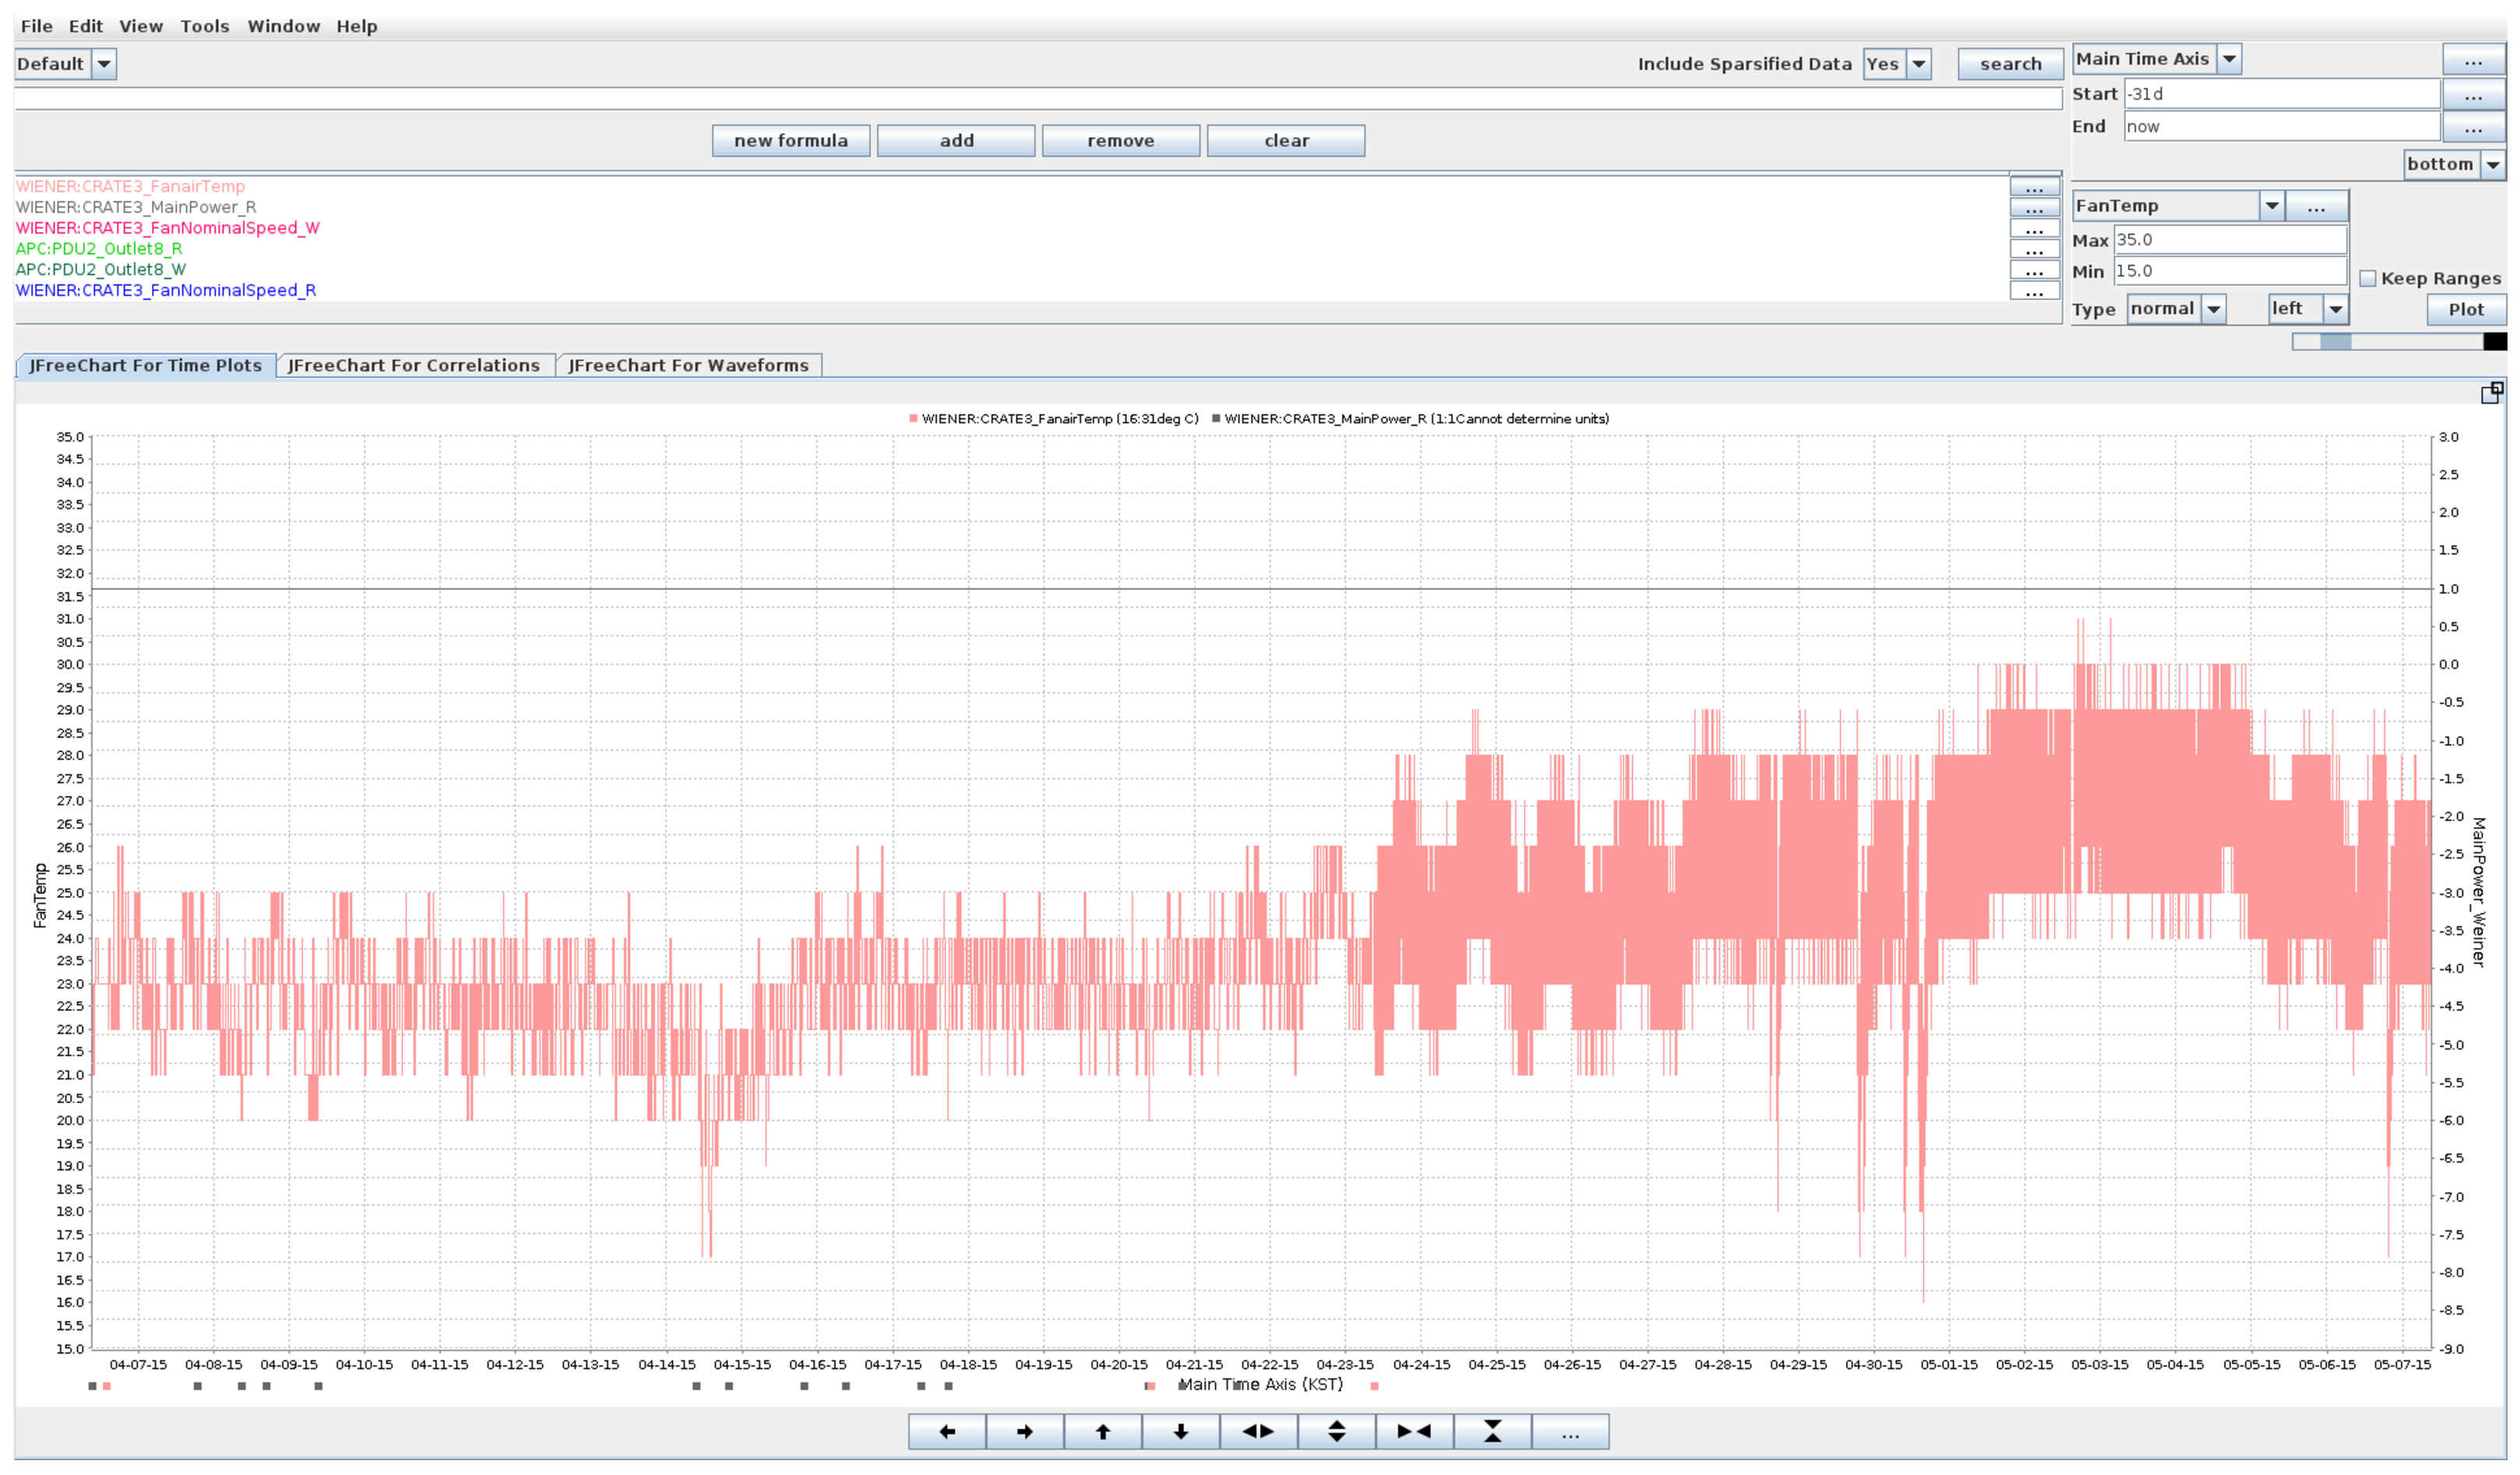
\includegraphics[width=0.99\textwidth]{./images/0507_archiver_wiener_temp_power.eps}
  \caption{Archiver Appliance Viewer}
  \label{fig:wienerv3}   
\end{figure}

\clearpage

\subsubsection{Wiener사 Crate의 SNMPv3 안정성}

앞서 확인한 IOC의 안정성과 달리 Wiener사의 SNMPv3는 그림 \ref{fig:issue}과 같은 문제가 발생하였다. 이는 하루 동안 IOC의 안정성을 테스트한 결과로 PDU Outlet 8번의 전원 On/Off, Wiener 전원, 팬 온도는 문제없이 Script에 의해 동작함을 알 수 있다. 그러나 팬 스피드는 Script에서 caput으로 FanNominalSpeed\_W값을 변경하지만, 어느 순간부터 FanNominalSpeed\_R가 값의 변화를 인지하지 못하는 문제가 발생한다. 이 문제가 발생하면 IOC는 계속해서 동작하지만, Wiener Crate의 PV가 caput, dbpf로 설정하는 값의 변화를 인지하지 않으며, 이 문제는 IOC를 재시작하는 방법으로만 해결된다.


\begin{figure}[h!]
  \centering
  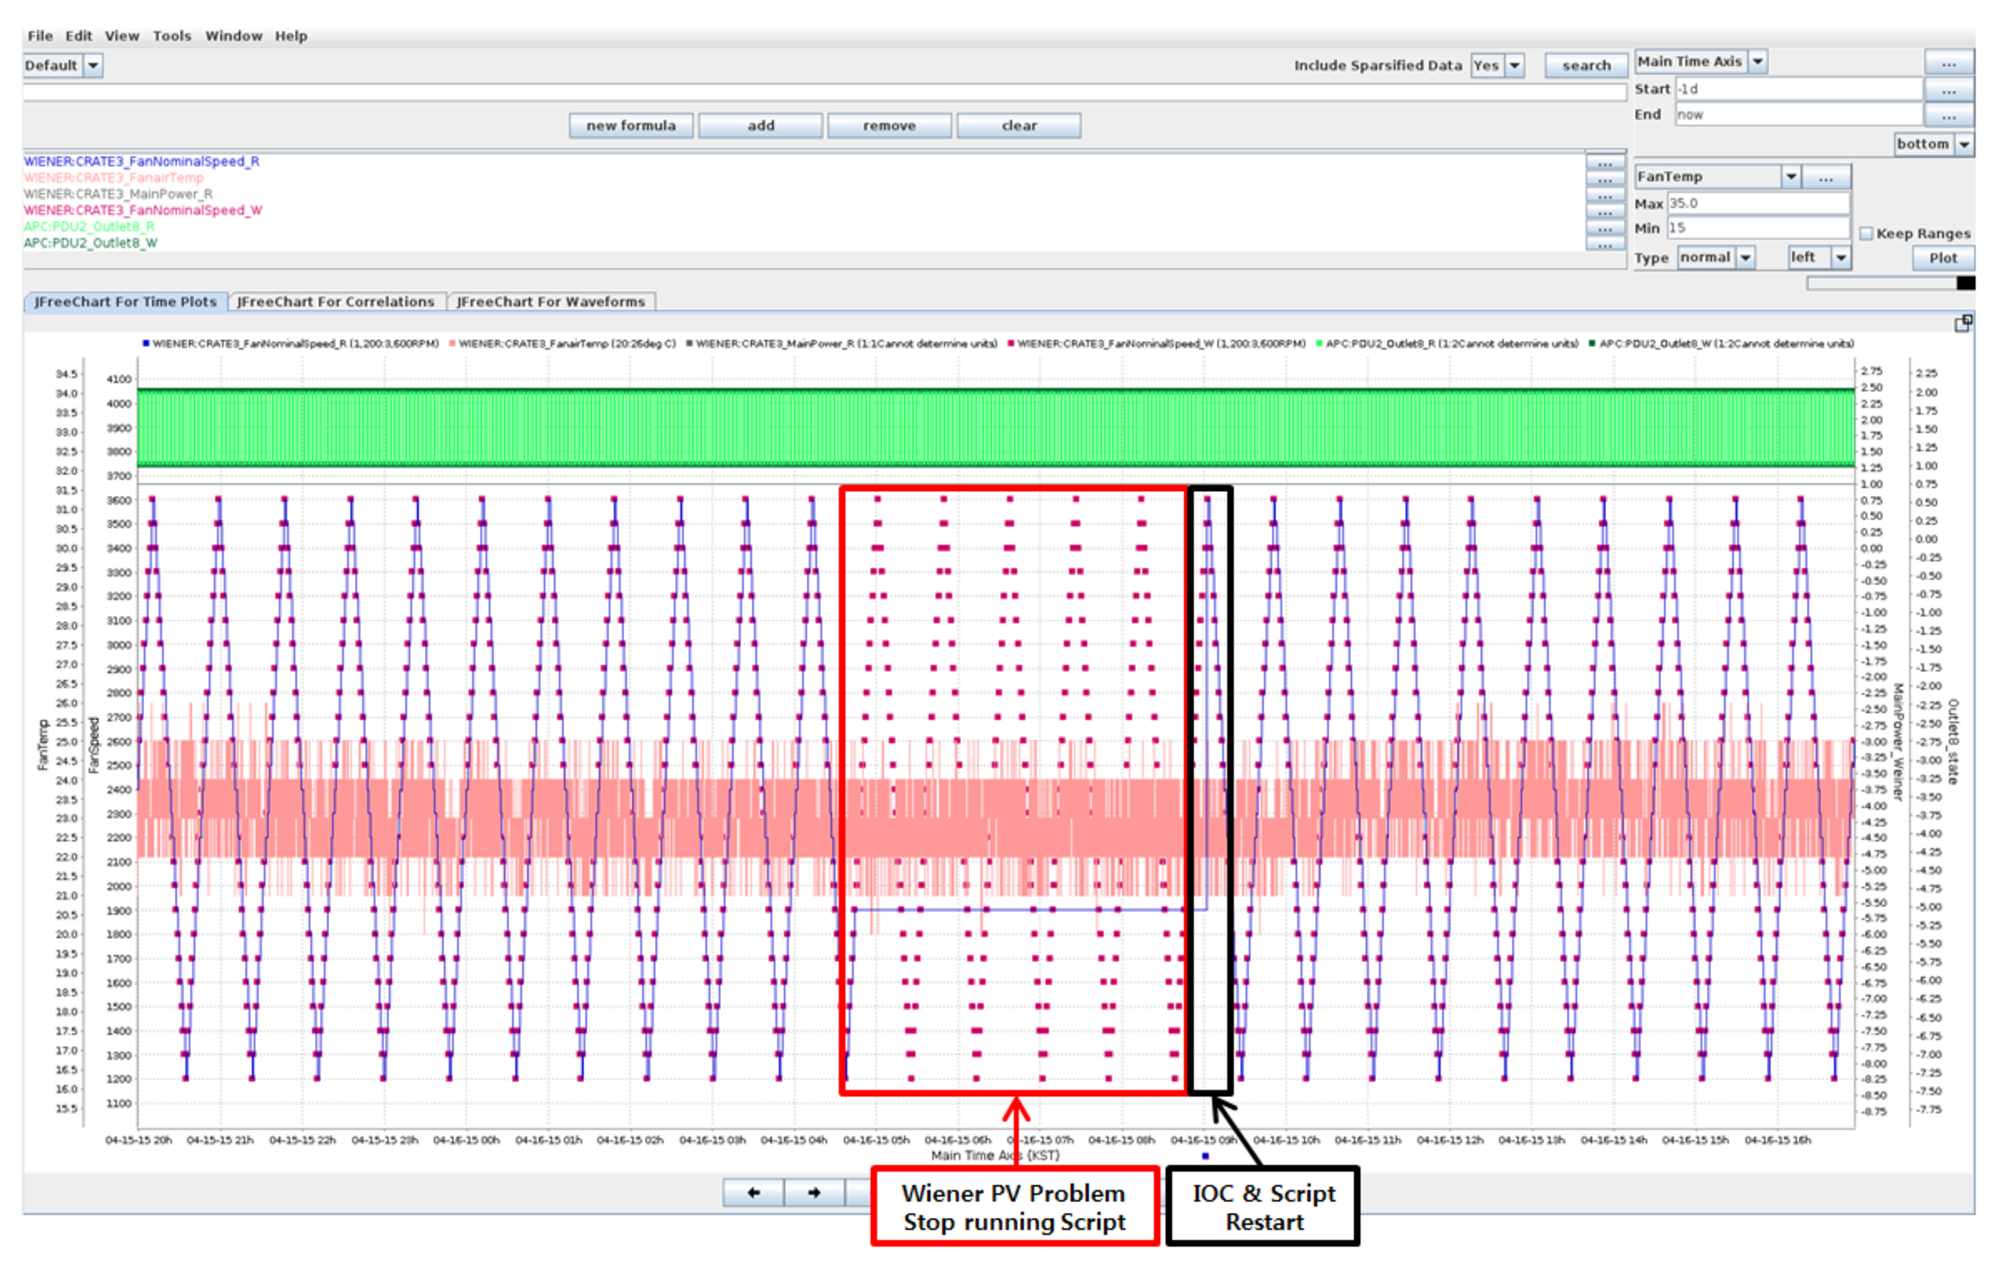
\includegraphics[width=0.99\textwidth]{./images/issueioc.eps}
  \caption{Wiener Crate 안정성 테스트 결과}
  \label{fig:issue}   
\end{figure}

\clearpage
이 문제가 주기적으로 발생하는지 확인하기 위해 IOC가 정상 동작한 시간을 정리하였다. 표 \ref{table:test1}는 30초 간격으로 팬 스피드를 1,200~3,000rpm 범위로 Script를 실행했을 때, 표 \ref{table:test2}는 1분 간격으로 1,200~3,600rpm 범위로 Script를 실행했을 때, IOC를 실행시킨 시간과 문제가 발생한 시간을 계산하여 IOC가 동작한 총 시간을 나타낸 것이다. 이를 참조하면 IOC문제가 주기적으로 발생하는 것이 아니며, 대부분 사람의 네트워크 접속이 거의 없는 시간대에서 IOC가 더 오래 동작했다는 점을 알 수 있다.


\begin{table}[h!]
\begin{center}
\small 
\begin{tabulary}{\textwidth}{C|C|C|C}
$ \sharp $ & IOC Run & IOC issue & IOC Running time\\ \hline
1 & 14:40:05 & 02:18:53 & 16:58:58 \\ \hline
2 & 09:01:36 & 14:43:28 & 05:41:52\\ \hline
3 & 16:55:01 & - & \\ 
  & - & 08:55:46 & 16:00:45\\ \hline
4 & 09:13:45  & - & \\ 
  & - & 03:07:45  & 17:54:00 \\
\end{tabulary}
\caption{안정성 테스트 결과(30s/1,200~3,000rpm)}
  \label{table:test1} 
\end{center}
\end{table} 


\begin{table}[h!]
\begin{center}
\small 
\begin{tabulary}{\textwidth}{C|C|C|C}
$ \sharp $ & IOC Run & IOC issue & IOC Running time\\ \hline
1 & 19:54:20  & - & \\ 
  & - & 10:34:17 & 14:39:57 \\ \hline
2 & 19:46:20 & - & \\ 
  & - & 04:46:26 & 9:00:06 \\ \hline
3 & 09:02:52 & 22:58:34 & 13:55:42 \\ \hline
4 & 09:10:06 & 17:10:48 & 08:00:42\\ \hline
5 & 17:43:39  & - & \\ 
  & - & 11:22:17  & 17:38:38 \\
\end{tabulary}
\caption{안정성 테스트 결과(60s/1,200~3,600rpm)}
  \label{table:test2} 
\end{center}
\end{table} 

이에 Crate가 네트워크 부하 영향을 받는 것인지 스위치에 연결된 네트워크의 문제인지 확인하기 위해 APC사의 PDU와 Wiener Crate의 IP주소를 바꿔 테스트를 진행해 보았다. 그러나 표 \ref{table:test3}의 결과와 같이 Crate에서의 문제는 계속되었다.

\begin{table}[h!]
\begin{center}
\small 
\begin{tabulary}{\textwidth}{C|C|C|C}
$ \sharp $ & IOC Run & IOC issue & IOC Running time\\ \hline
1 & 10:17:39 & 17:59:14 & 07:41:35 \\ \hline
2 & 19:48:01 & - & \\ 
  & - & 12:11:32 & 16:23:31\\ \hline
3 & 13:23:17  & - & \\ 
  & - & 06:23:01  & 16:59:44 \\
\end{tabulary}
\caption{안정성 테스트 결과(60s/1,200~3,600rpm/IP 변경)}
  \label{table:test3} 
\end{center}
\end{table} 

\clearpage

추가로 하나의 IOC에서 두 개의 장비가 실행되는 것이 문제인지 확인하기 위해 아래와 같이 PDU와 Crate의 IOC를 분리하여 테스트를 진행하였으나 Crate에서 문제는 그림 \ref{fig:issue2}과 같이 계속 발생하였다.

{\scriptsize
\begin{verbatim}
.
├── [mijoy090  134]  envPaths
├── [mijoy090  124]  Makefile
├── [mijoy090 1.0K]  st.cmd
├── [mijoy090  762]  st.cmd.apc7921
└── [mijoy090  795]  st.cmd.wiener6023

\end{verbatim}
}

\begin{figure}[h!]
  \centering
  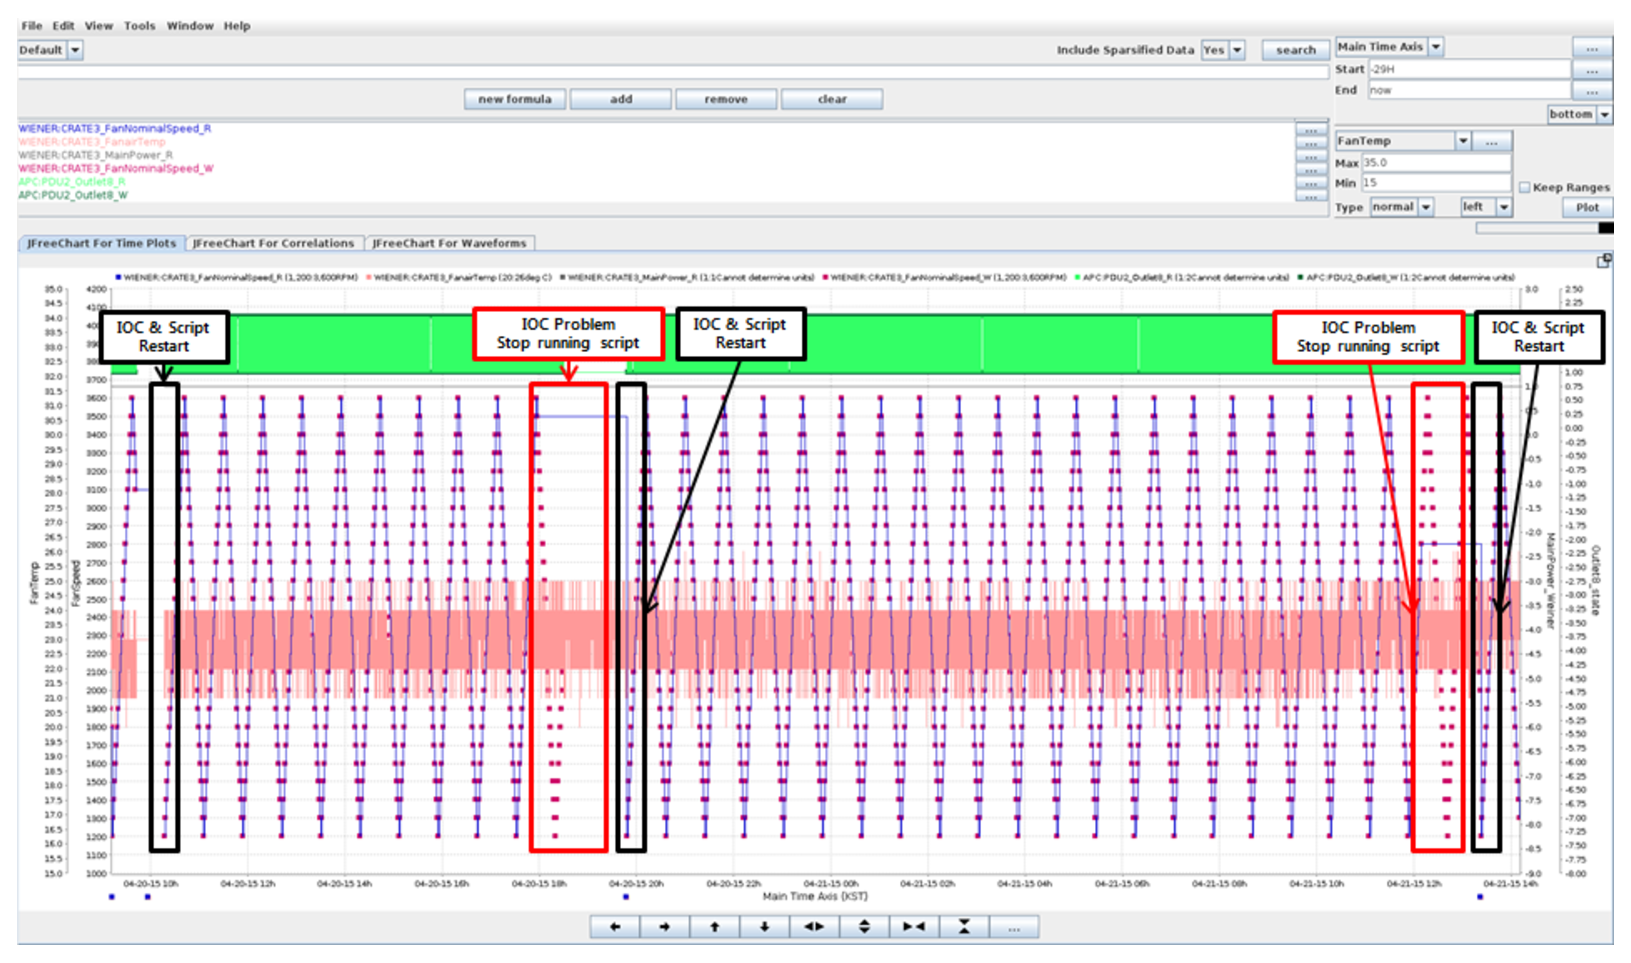
\includegraphics[width=0.99\textwidth]{./images/issue2.eps}
  \caption{IOC 분리 후 Wiener Crate 안정성 테스트 결과}
  \label{fig:issue2}   
\end{figure}

따라서 같은 형태로 SNMPv2c로 Read, v3으로 Write하는 PDU Outlet 8번과 v2c로 Read하는 Wiener사 Crate의 팬 온도와 전원상태와 비교해 Crate의 팬 스피드에서만 발생하는 이 문제는 SNMPv3를 지원한 지 얼마 안 된 Wiener사의 SNMP 문제인지, IOC의 문제인지 추가적인 확인이 필요하다. 또한, IOC의 장기적인 안정성 테스트도 요구된다.



\clearpage
\bibliographystyle{unsrtnat}
\bibliography{./refs}


\end{document}
